%-----------------------------------------------------------------------------------------------%
%
% Maret 2019
% Template Latex untuk Tugas Akhir Program Studi Sistem informasi ini
% dikembangkan oleh Inggih Permana (inggihjava@gmail.com)
%
% Template ini dikembangkan dari template yang dibuat oleh Andreas Febrian (Fasilkom UI 2003).
%
% Orang yang cerdas adalah orang yang paling banyak mengingat kematian.
%
%-----------------------------------------------------------------------------------------------%

%-----------------------------------------------------------------------------%
\chapter{\babDua}
%-----------------------------------------------------------------------------%

%-----------------------------------------------------------------------------%
\section{Penelitian Terdahulu}
%-----------------------------------------------------------------------------%

Penggunaan standar ISO 9126 dalam evaluasi sistem inventaris dan aplikasi berbasis web telah menjadi fokus beberapa penelitian di berbagai institusi pendidikan di Indonesia. Salah satu studi penting dilakukan di ISB Atma Luhur, di mana peneliti mengevaluasi sistem inventaris laboratorium menggunakan empat aspek utama ISO 9126: functionality, usability, reliability, dan efficiency. Metodologi penelitian ini melibatkan penggunaan kuesioner yang didistribusikan kepada para pengguna sistem untuk menilai seberapa baik fungsi sistem berjalan. Data yang diperoleh kemudian dianalisis menggunakan metode perhitungan nilai untuk menentukan persentase keberhasilan, terutama pada aspek functionality \cite{alkodri2023pengaplikasian}.

Melanjutkan perkembangan ini, sebuah studi di Universitas Negeri Yogyakarta memperluas cakupan evaluasi dengan fokus pada aplikasi berbasis web. Penelitian ini menggali lebih dalam aspek functionality dan reliability. Untuk menguji functionality, para peneliti menggunakan pendekatan inovatif dengan pernyataan "ya-tidak" untuk menentukan apakah setiap fungsi utama sistem berfungsi dengan baik. Sementara itu, aspek reliability diuji menggunakan alat LoadImpact, yang memungkinkan pengukuran performa aplikasi di bawah beban tinggi, memberikan wawasan berharga tentang ketahanan sistem dalam situasi yang menantang \cite{dewi2017quality}

Kontribusi signifikan lainnya datang dari penelitian yang dilakukan di Institut Teknologi Nasional Malang. Studi ini menambahkan dimensi baru dalam evaluasi sistem informasi inventaris dengan menggabungkan pengujian functionality, reliability, dan maintainability. Khusus untuk aspek functionality, penelitian ini berfokus pada pengukuran apakah semua fitur berjalan sesuai yang diharapkan. Yang menarik, untuk evaluasi reliability, peneliti menggunakan metode stress testing dengan WAPT v10.1, memberikan gambaran yang lebih komprehensif tentang kinerja sistem dalam kondisi ekstrim \cite{kumalasari2024analisis}.

Seiring dengan perkembangan teknologi mobile, sebuah studi inovatif mengaplikasikan standar ISO 9126 pada sistem inventaris laboratorium berbasis Android. Penelitian ini tidak hanya mengevaluasi aspek functionality dan portability, tetapi juga memberikan perhatian khusus pada usability dengan menggunakan kuesioner SUPR-Q. Fitur unik dari sistem ini adalah integrasi pemantauan melalui CCTV, yang menambah nilai dengan menciptakan transparansi dan keamanan tambahan. Pendekatan ini menunjukkan bagaimana standar ISO 9126 dapat diadaptasi untuk teknologi modern dan kebutuhan pengguna yang berkembang.
Akhirnya, penelitian terbaru dalam bidang inventory management yang melibatkan penggunaan Android Studio semakin memperluas pemahaman kita tentang fleksibilitas ISO 9126 dalam menilai aplikasi lintas platform. Fokus utama diberikan pada aspek portability, di mana peneliti menguji kemampuan aplikasi untuk diakses dari berbagai perangkat, baik desktop maupun mobile. Studi ini menekankan pentingnya fleksibilitas akses dalam pengembangan sistem modern, terutama dalam konteks di mana pengguna perlu mengakses informasi inventaris dari berbagai lingkungan dan perangkat \cite{alkodri2023pengaplikasian}.

Secara keseluruhan, rangkaian penelitian ini menunjukkan evolusi penggunaan ISO 9126 dalam evaluasi sistem inventaris, dari aplikasi berbasis web tradisional hingga solusi mobile modern. Masing-masing studi memberikan perspektif unik dan memperkaya pemahaman kita tentang bagaimana standar ini dapat diterapkan secara efektif dalam berbagai konteks teknologi dan kebutuhan institusional. Keragaman pendekatan dan fokus dalam penelitian-penelitian ini juga menegaskan fleksibilitas dan relevansi berkelanjutan dari ISO 9126 sebagai kerangka kerja untuk evaluasi kualitas perangkat lunak.
%-----------------------------------------------------------------------------%
\section{Profil Instansi}
\begin{longtable}{lll}
	Perguruan Tinggi & : & UIN Suska Riau \\
	\endfirsthead
	%
	\multicolumn{3}{c}%
	{{\bfseries Lanjutan dari halaman sebelumnya}} \\
	Perguruan Tinggi & : & UIN Suska Riau \\
	\endhead
	%
	Fakultas & : & Sains dan Teknologi \\
	Program Studi & : & Sistem Informasi \\
	Jenjang & : & Strata 1 (S1) \\
	No. SK Pendirian Program Studi & : & DJ.II/26/2006 \\
	SK Penyelenggaraan & : & 3480/D/T/K-AI/2009 \\
	Tanggal SK Pendirian Program Studi & : & 20 Februari 2006 \\
	Pejabat Penandatangan SK & : & Direktur Jenderal Perguruan Tinggi \\
	Penyelenggaraan Program Studi & : & Juli 2002 \\
	Nomor SK Izin Operasional & : & Dj.I/123/2012 \\
	Tanggal SK Izin Operasional & : & 25 Januari 2012 \\
	Akreditasi Program Studi & : & Baik Sekali \\
	Keberlakuan Akreditasi & : & 19 Maret 2024 - 19 Maret 2029 \\
	Nomor SK LAM INFOKOM & : & 018/SK/LAM-INFOKOM/Ak/S/III/2024 \\
	Email & : & faste.sif@uin-suska.ac.id \\
	Website & : & https://sif.uin-suska.ac.id/ \\
	Alamat & : & \begin{tabular}[c]{@{}l@{}}Jl. HR. Soebrantas No. 155 KM 15, \\ Pekanbaru 28293.\end{tabular}
	\end{longtable}
%-----------------------------------------------------------------------------%
\subsection{Sejarah}
%-----------------------------------------------------------------------------%
UIN Suska Riau memiliki fasilitas infrastruktur pendukung Tridharma Perguruan Tinggi yang baik, salah satunya adalah laboratorium terpadu di bawah Fakultas Sains dan Teknologi yang dikelola oleh Program Studi Sistem Informasi sejak tahun 2002. Terdapat tiga laboratorium yang dikelola oleh Program Studi Sistem Informasi, yaitu Laboratorium Rekayasa Sistem Informasi (RSI), Laboratorium Internet (INT), dan Laboratorium \textit{Software Engineering} (SE). Ketiga laboratorium tersebut merupakan aset penting yang dapat dimanfaatkan dengan baik untuk mencapai target-target universitas dan menghasilkan lulusan Program Studi Sistem Informasi yang kompeten dalam pendidikan, penelitian, serta pengabdian masyarakat dengan mengintegrasikan nilai-nilai keislaman. Laboratorium-laboratorium tersebut tidak hanya digunakan untuk praktikum mahasiswa sesuai dengan kurikulum, tetapi juga mampu mendukung berbagai kegiatan mahasiswa dan dosen dalam meningkatkan pengetahuan di bidang Sistem Informasi.
% -----------------------------------------------------------------------------%
\subsection{Visi}
% -----------------------------------------------------------------------------%
Menjadi laboratorium Program Studi Sistem Informasi yang memiliki keunggulan dalam bidang pendidikan, penelitian, dan pengabdian kepada masyarakat dengan menghasilkan lulusan yang proaktif, inovatif, dan profesional dalam bidang Sistem Informasi di tingkat lokal, regional, dan nasional yang berbasis nilai-nilai islami pada tahun 2030.
% -----------------------------------------------------------------------------
\subsection{Misi}
% -----------------------------------------------------------------------------%
Untuk mencapai Visi Laboratorium Program Studi Sistem Informasi, berikut Misi-misi yang harus dicapai, diantaranya:

\begin{enumerate}

  \item Mendukung penyelenggaraan kegiatan pendidikan akademik dan praktikum berbasis teknologi kepada mahasiswa, dosen, dan stakeholder.
  \item Mendukung pelaksanaan kegiatan penelitian yang berbasis teknologi kepada mahasiswa, dosen, dan stakeholder.
  \item Mendukung kegiatan pengabdian kepada masyarakat yang berbasis teknologi.
  \item Menyiapkan sumber daya manusia yang mampu menerapkan teknologi informasi khususnya dibidang Sistem Informasi.
  \item Membangun kemitraan dan jejaring dengan industri, pemerintah, dan organisasi nasional.

\end{enumerate}
% -----------------------------------------------------------------------------%
\subsection{Struktur Organisasi}
% -----------------------------------------------------------------------------%
Untuk menjalankan Tridharma Perguruan Tinggi dengan baik, pengelola laboratorium harus memiliki kemampuan manajerial yang baik dan dibantu dengan keahlian IT. Untuk mencapai hal ini, diperlukan sekelompok pengelola laboratorium yang percaya diri dan memiliki kemampuan. Gambar 2.1 menunjukkan struktur organisasi pengelola laboratorium Program Studi Sistem Informasi dari 2021 hingga 2024.

\begin{figure}
  \centering
  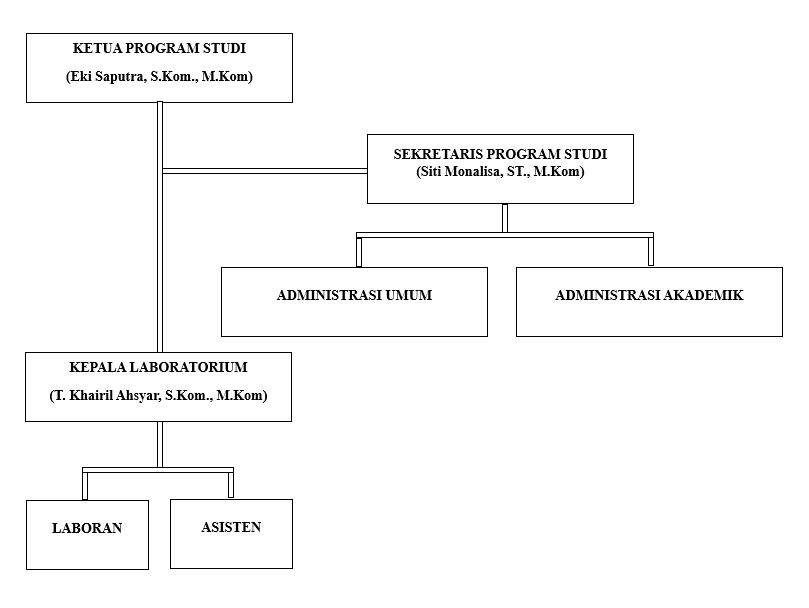
\includegraphics[width=0.82\linewidth]{konten//gambar/Struktur Organisasi.png}
  \caption{Struktur Organisasi Laboratorium}
  \label{fig:enter-label}
\end{figure}

% -----------------------------------------------------------------------------%
\section{Sistem Informasi Inventaris}
% -----------------------------------------------------------------------------%
Sistem informasi adalah suatu sistem didalam Organisasi yang mempertemukan kebutuhan pengolahan transaksi harian, mendukung operasi bersifat manajerial dan kegiatan strategi dari suatu organisasi dan menyediakan pihak luar tertentu dengan laporan-laporan yang diperlukan \cite{laila2011sistem}. Sistem informasi inventaris adalah suatu sistem yang digunakan untuk mengelola dan memantau inventaris atau barang yang dimiliki oleh suatu organisasi atau perusahaan. Sistem ini dapat membantu memudahkan petugas inventaris dalam pendataan barang yang dimiliki oleh organisasi atau perusahaan tersebut \cite{Yanti2021SISTEMII}.
%-----------------------------------------------------------------------------%
%-----------------------------------------------------------------------------%
\section{Laboratorium}
Laboratorium merupakan sarana dalam melaksanakan sebuah riset dalam bidang ilmiah, eksperimen, pengukuran maupun pelatihan ilmiah. Meski laboratorium telah memiliki alat-alat yang lengkap, pengelolaan laboratorium juga harus diperhatikan. Adanya alat-alat yang sudah lengkap dan penggunaan yang sudah baik tentunya perlu untuk dilakukan manajemen yang baik pada laboratorium tersebut, karena terdapat beberapa hal yang harus diperhatikan kembali seperti pengelolaan masing-masing laboratorium dan pengolahan data \cite{sweden2022rancang}.

\subsection{Laboratorium Rekayasa Sistem Informasi (RSI)}
Laboratorium Rekayasa sistem Informasi atau yang disingkat dengan nama Laboratorium RSI merupakan laboratorium pertama yang dimiliki oleh Program Studi Sistem Informasi sejak pindahnya aktivitas perkuliahan kampus dari kampus Sukajadi ke kampus utama Panam Pekanbaru Riau pada tahun 2007. Fungsi utama dari laboratorium ini adalah sebagai fasilitas infrastruktur pendukung untuk pelaksanaan kegiatan perkuliahan praktikum bagi mahasiswa Program Studi Sistem Informasi terkait bidang Rekayasa Sistem Informasi. Bidang Rekayasa Sistem Informasi merupakan bidang yang paling dominan yang ada di Program Studi Sistem Informasi \cite{lab-si-website}.

\subsection{Laboratorium Internet (INT)}
Laboratorium Internet atau yang disingkat dengan nama Laboratorium INT merupakan laboratorium milik Program Studi Sistem Informasi di bawah Fakultas Sains dan Teknologi kedua yang aktivitas perkuliahannya berada di kampus utama Panam Pekanbaru Riau. Secara spesifik, laboratorium ini lebih dioperasikan untuk kebutuhan perkuliahan terkait matakuliah praktikum dasar, seperti matakuliah Jaringan Komputer dan Pemrograman Dasar \cite{lab-si-website}.

\subsection{Laboratorium \textit{Software Engineering} (SE)}
Laboratorium ke tiga yang dimiliki oleh Program Studi Sistem Informasi adalah Laboratorium \textit{Software Engineering} atau yang disingkat dengan nama Laboratorium SE. Laboratorium ini merupakan laboratorium terbaru milik yang dikelola oleh Program Studi dari usulan pengadaan barang tahun anggaran 2021 di bawah naungan Fakultas Sains dan Teknologi UIN Suska Riau. Adapun laboratorium SE sebagai pendukung dalam pelaksanaan kegiatan perkuliahan praktikum bagi mahasiswa Program Studi Sistem Informasi yang terkait dengan bidang keilmuan seperti Praktikum Basis Data, Pemrograman Beorientasi Objek (PBO), dan matakuliah wajib praktikum lainnya \cite{lab-si-website}.

\section{SITARIS SI}

Sistem Informasi Inventaris Laboratorium adalah sebuah platform yang dibuat dengan menggunakan Framework CodeIgniter4 dan bahasa pemrograman PHP yang dimaksudkan untuk membantu mengelola dan memantau inventaris barang dan peralatan laboratorium. Sistem ini memiliki potensi untuk meningkatkan efisiensi dan produktivitas dalam operasional laboratorium berkat berbagai fitur utama yang ditawarkannya.

Dengan adanya sistem ini, diharapkan pengelolaan inventaris laboratorium menjadi lebih mudah dan efisien, sehingga staf laboratorium dapat fokus pada tugas yang lebih penting. Selain itu, laporan yang dihasilkan oleh sistem dapat membantu dalam pengambilan keputusan yang lebih baik tentang persediaan barang dan peralatan laboratorium \cite{sitaris-lab-si-website}. SITARIS SI dapat diakses di alamat https://sitaris.lab-si.uin-suska.ac.id. Terdapat beberapa menu yang ada pada SITARIS SI, yaitu:

\begin{enumerate}
  \item Halaman \textit{login} \\ Halaman \textit{login} merupakan tampilan awal sistem ketika diakses. Terdapat formulir \textit{username} dan \textit{password} dan dilindungi oleh anti spam dari google reCAPTCHA yang digunakan untuk masuk ke dalam sistem informasi inventaris seperti pada Gambar 2.2.

        \begin{figure}
          \centering
          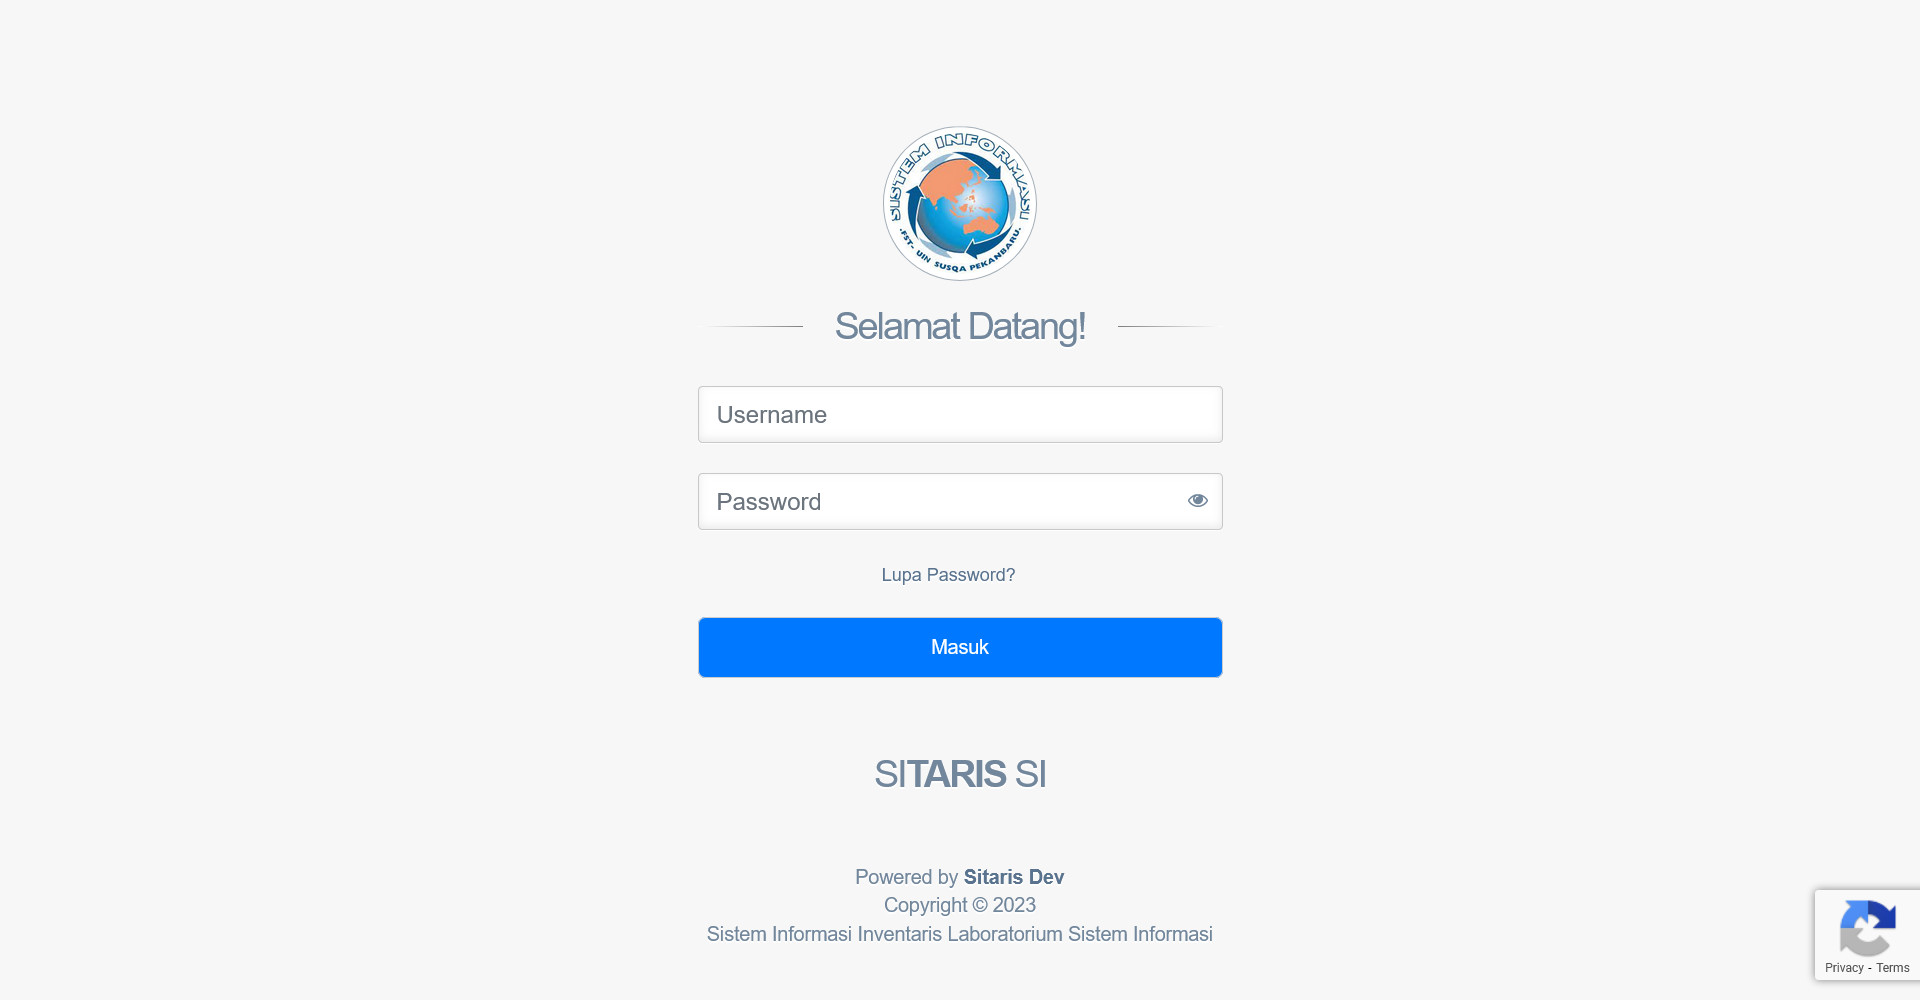
\includegraphics[width=0.82\linewidth]{konten//gambar/Login Page.png}
          \caption{Halaman \textit{Login}}
          \label{fig:enter-label}
        \end{figure}
        % Jika \textit{login} tidak berhasil maka akan menampilkan pesan seperti pada Gambar 4.66.

        % \begin{figure}
        %   \centering
        %   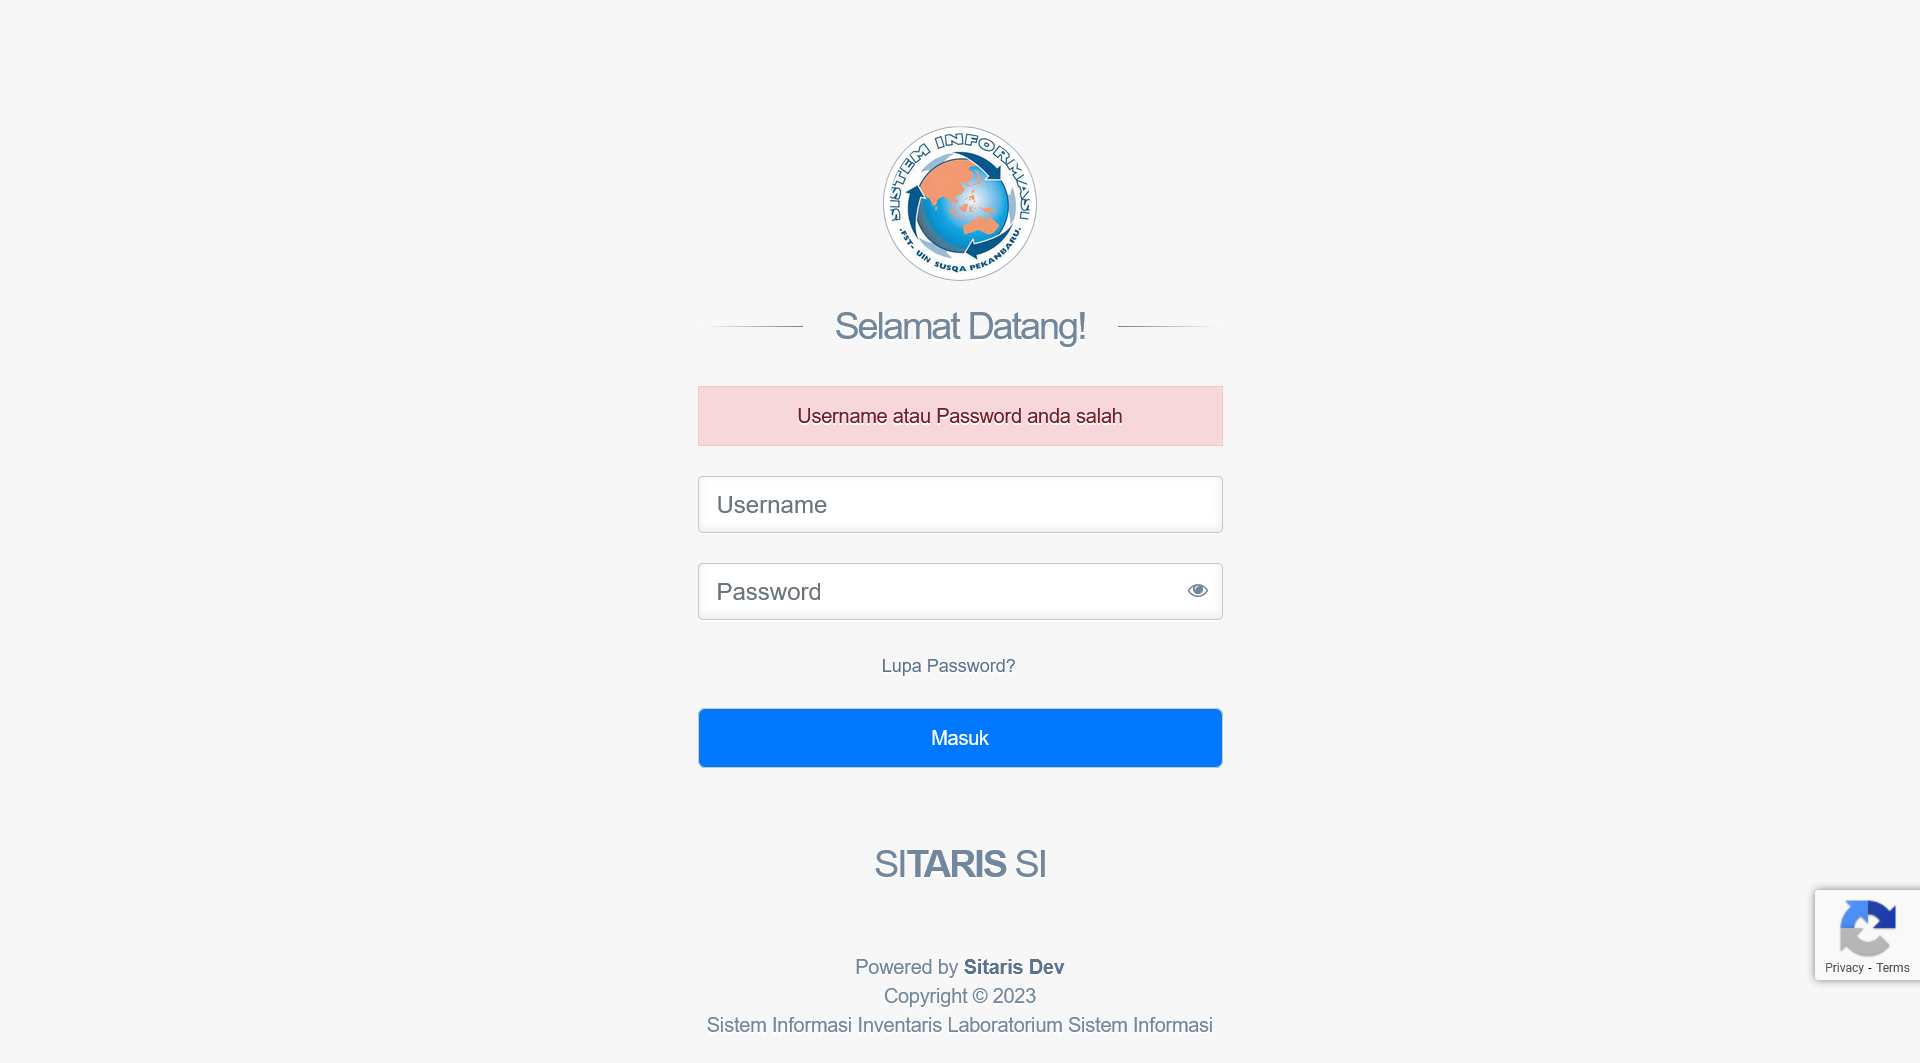
\includegraphics[width=0.82\linewidth]{konten//gambar/login gagal.png}
        %   \caption{Tampilan \textit{Login} gagal}
        %   \label{fig:enter-label}
        % \end{figure}

  \item Halaman Beranda \\ Halaman beranda merupakan tampilan awal yang ditampilkan kepada \textit{user} jika \textit{user} berhasil \textit{login} seperti pada Gambar 2.3.

        \begin{figure}
          \centering
          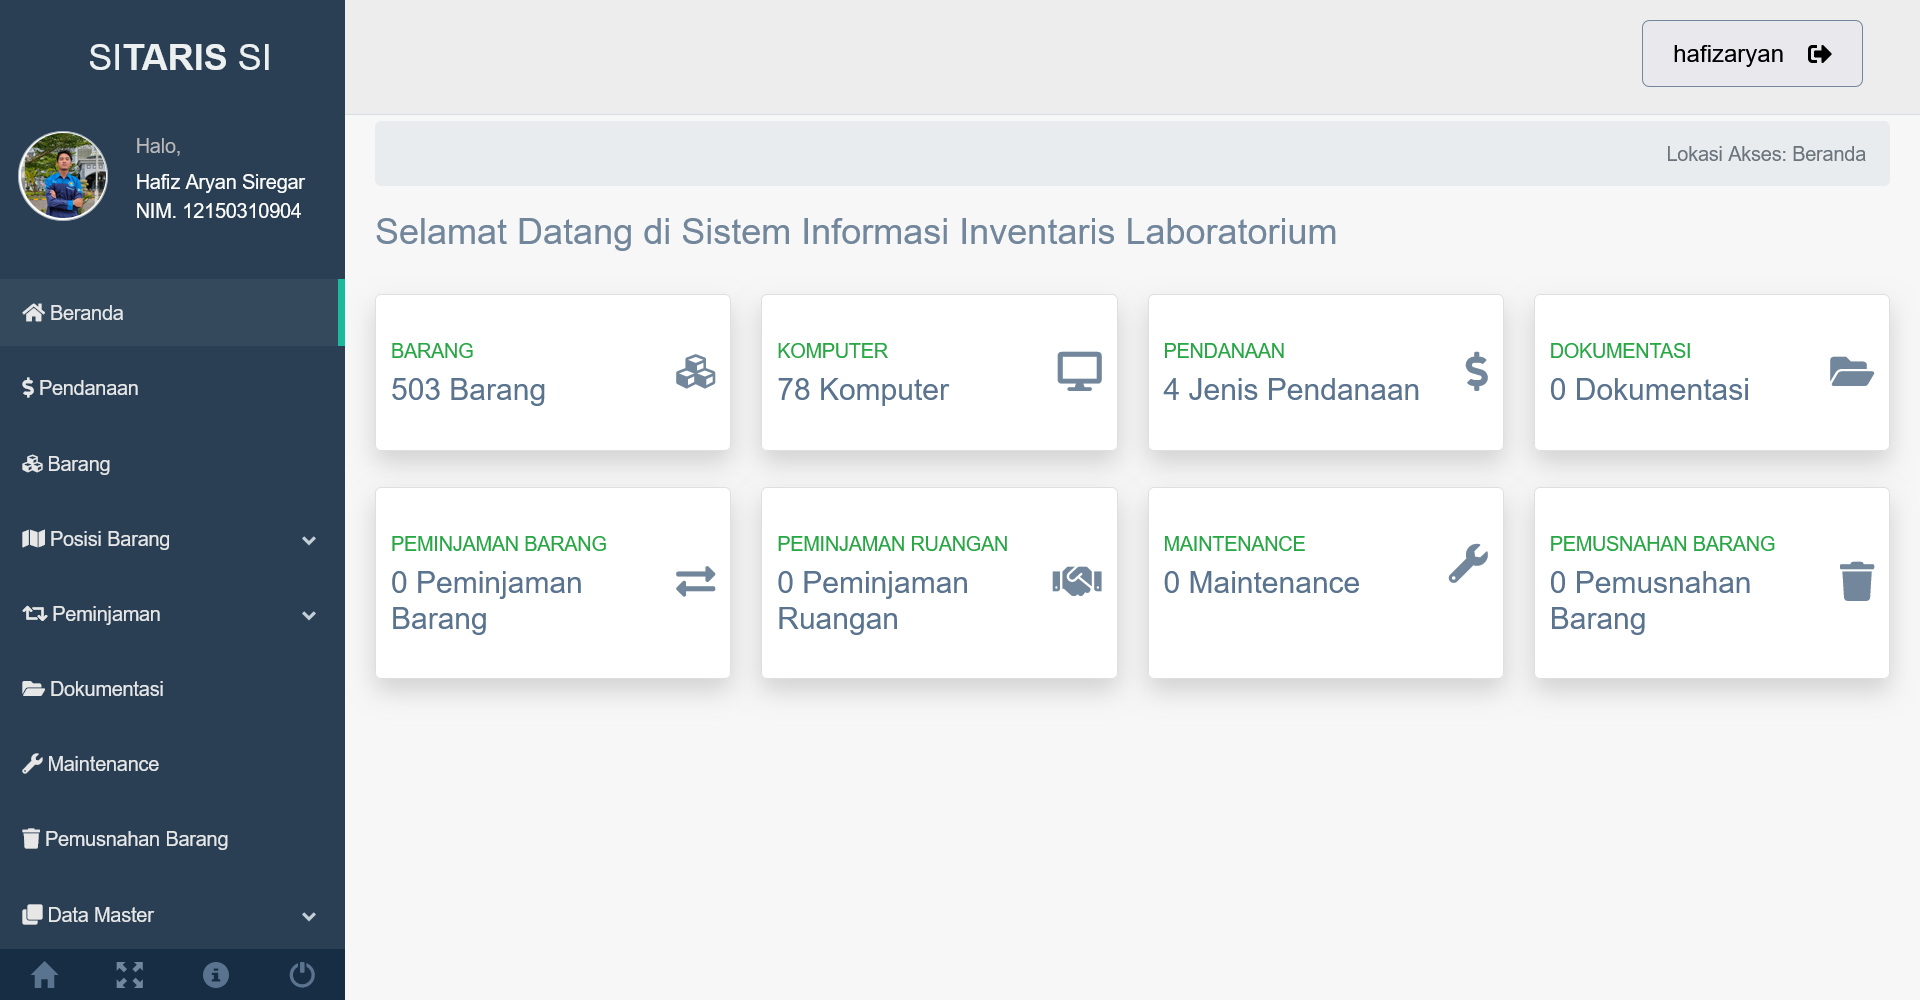
\includegraphics[width=0.82\linewidth]{konten//gambar/login berhasil.png}
          \caption{Halaman Beranda}
          \label{fig:enter-label}
        \end{figure}

        % Halaman beranda setiap pengguna berbeda-beda sesuai dengan hak akses yang diberikan, tampilan halaman beranda berdasarkan hak akses seperti pada Gambar 4.68. sampai Gambar 4.72.

        % \begin{figure}
        %   \centering
        %   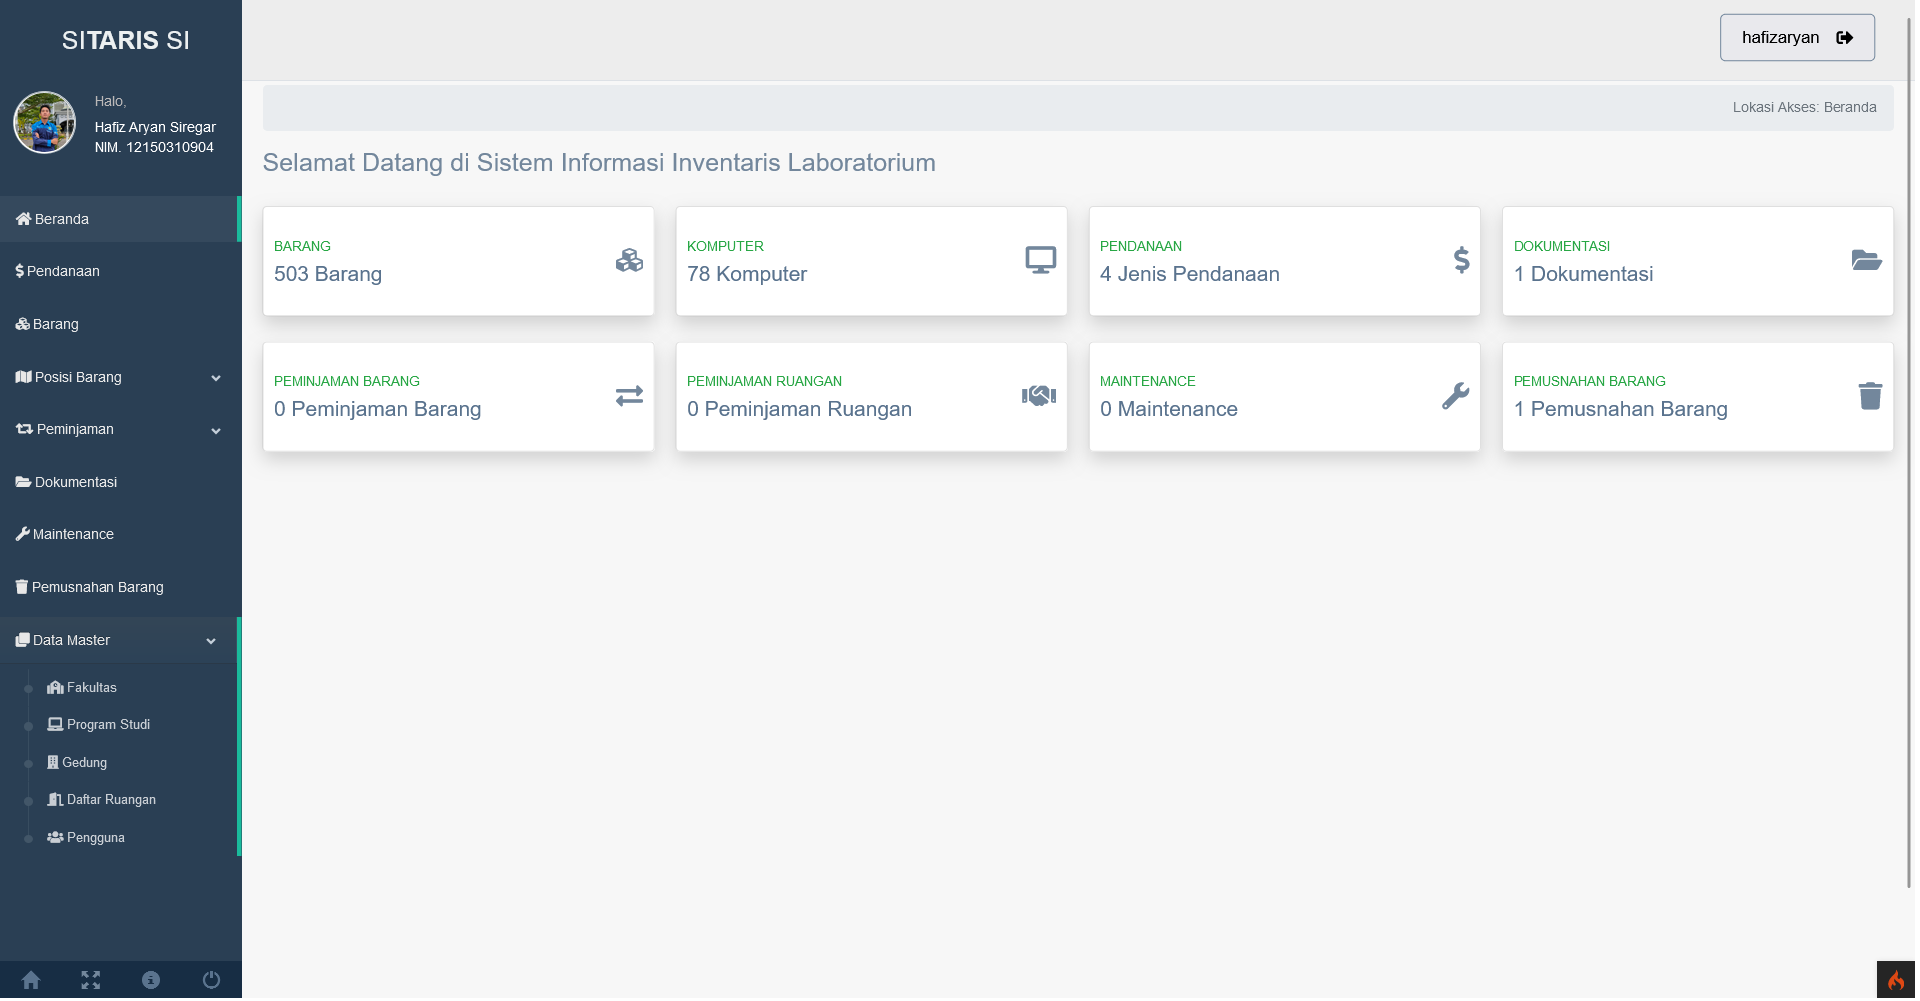
\includegraphics[width=0.82\linewidth]{konten//gambar/admin.png}
        %   \caption{Halaman Beranda Admin}
        %   \label{fig:enter-label}
        % \end{figure}

        % \begin{figure}
        %   \centering
        %   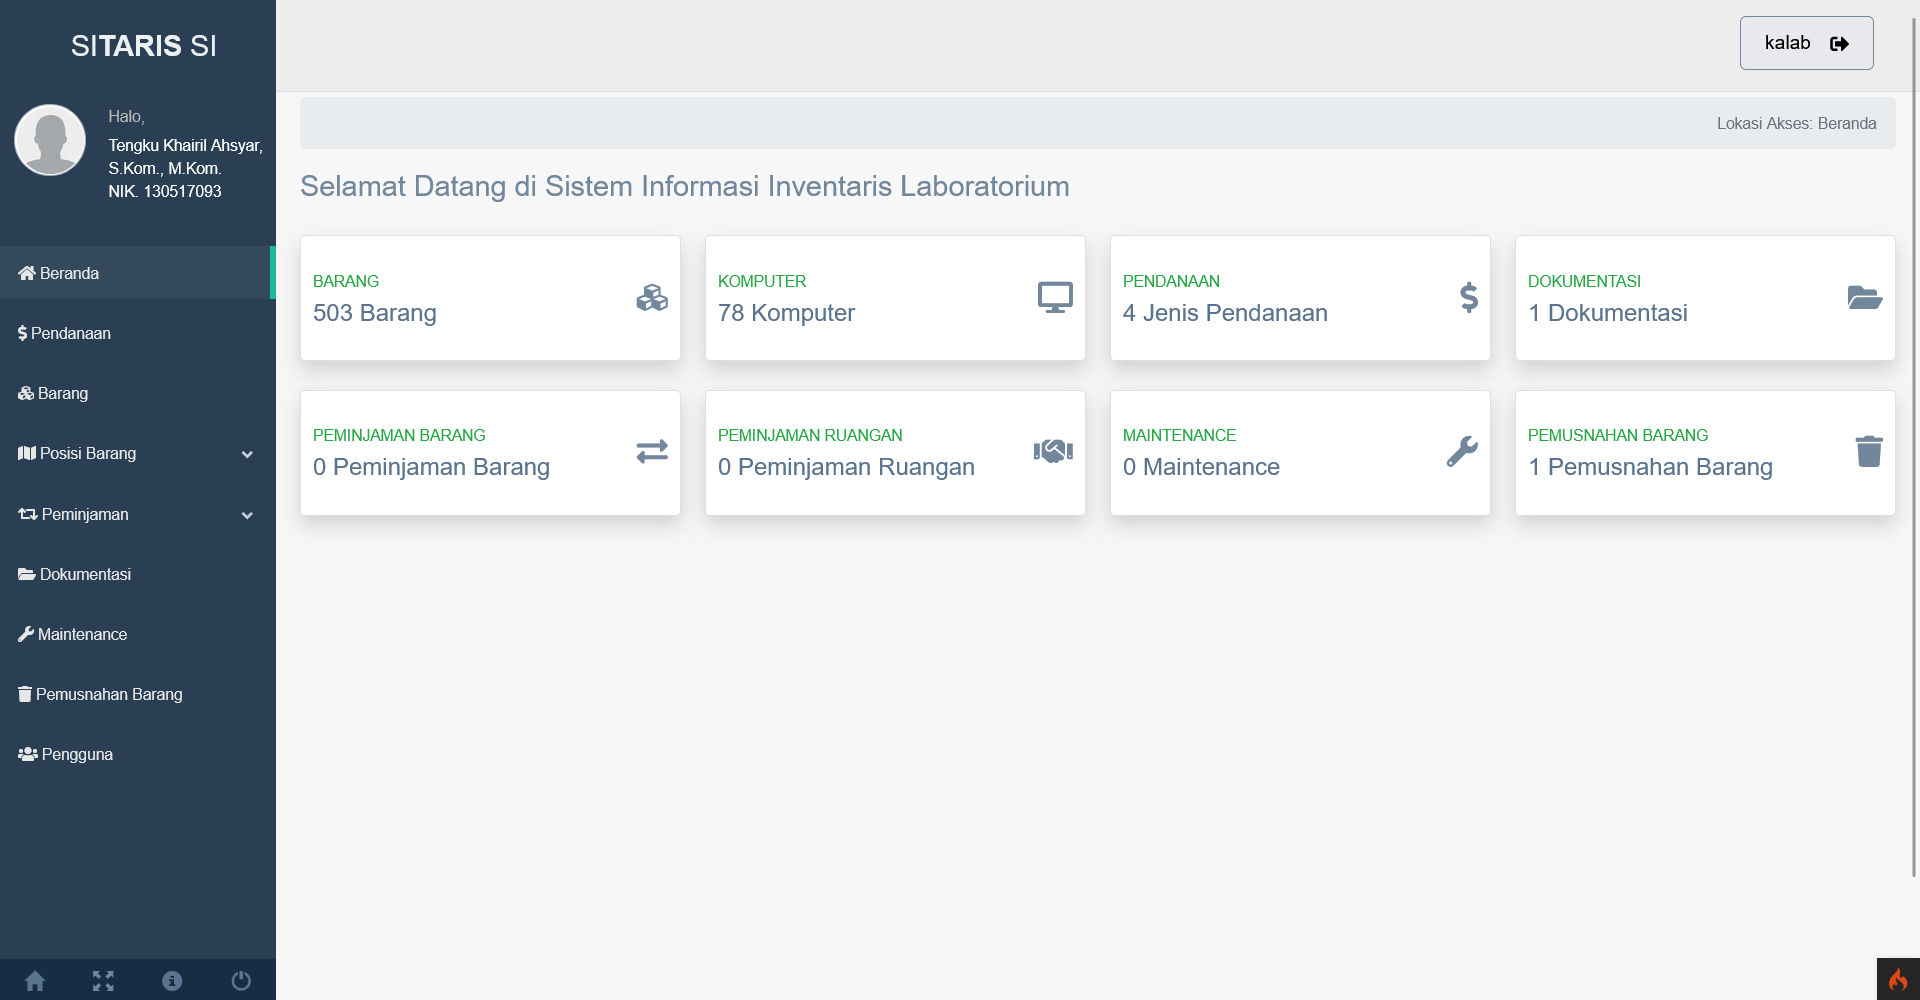
\includegraphics[width=0.82\linewidth]{konten//gambar/kalab.png}
        %   \caption{Halaman Beranda Kalab}
        %   \label{fig:enter-label}
        % \end{figure}

        % \begin{figure}
        %   \centering
        %   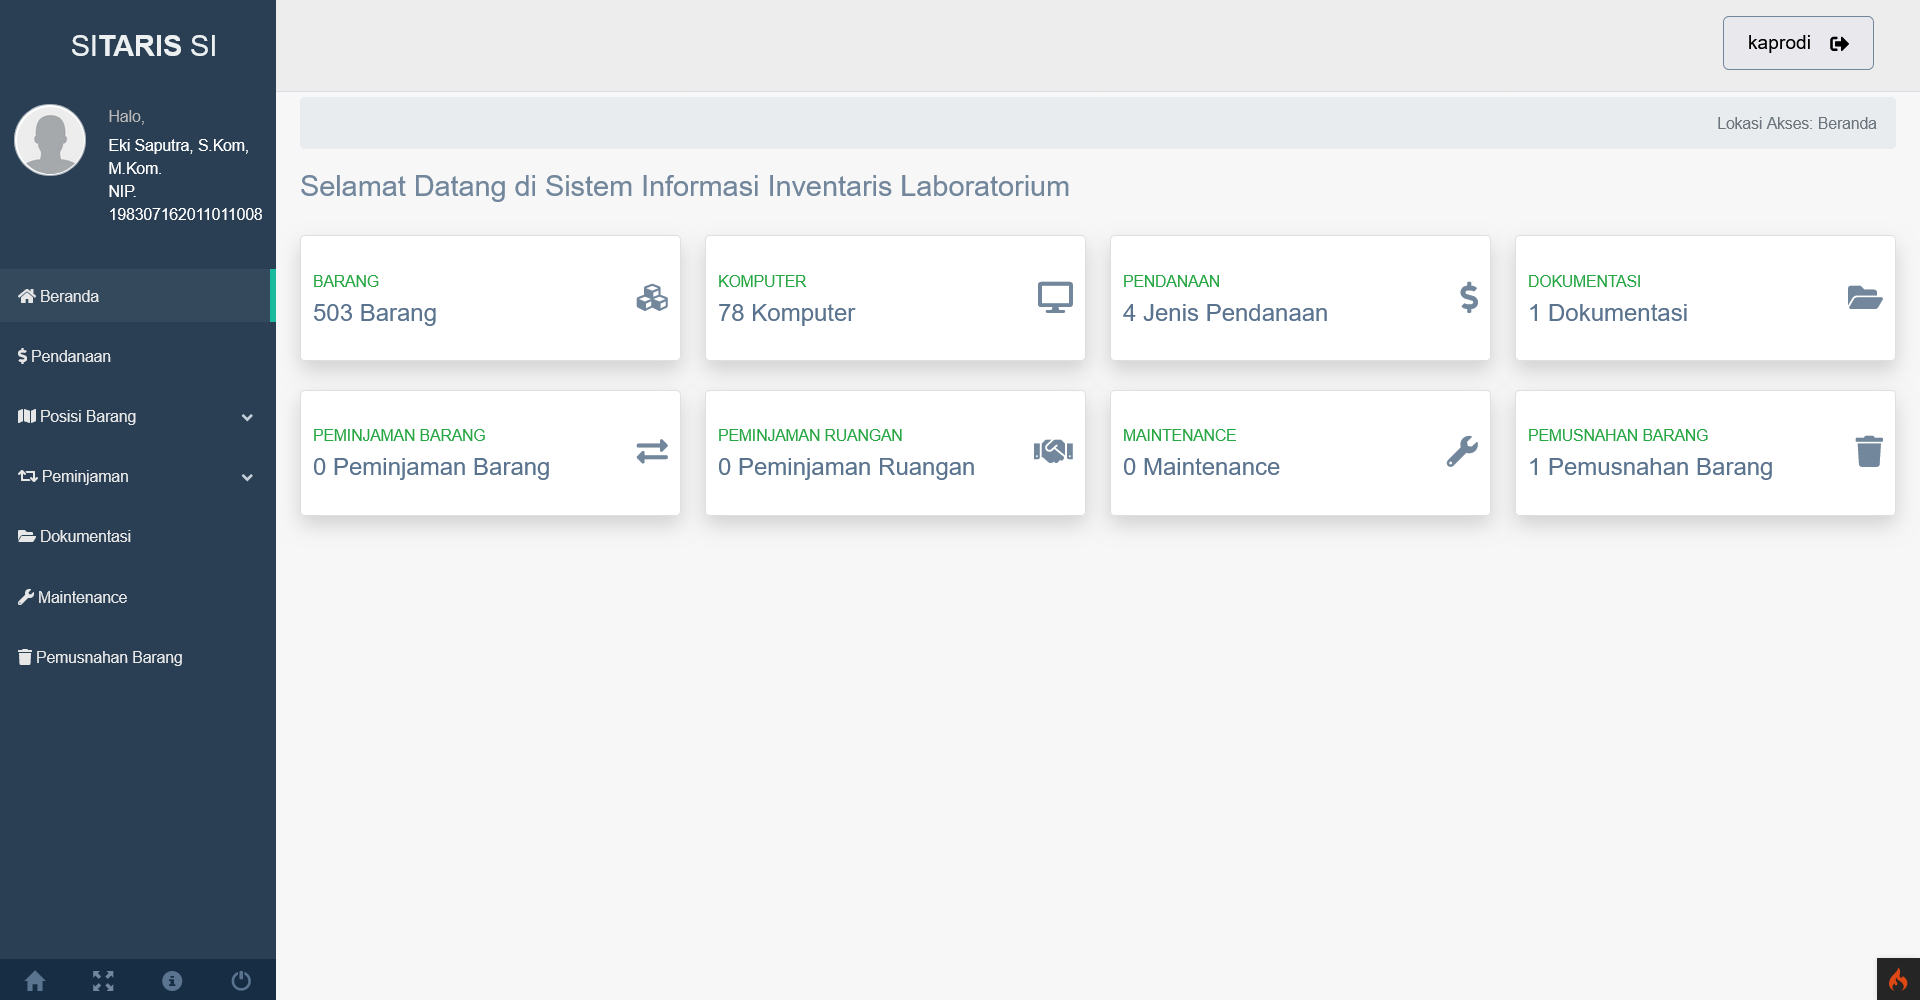
\includegraphics[width=0.82\linewidth]{konten//gambar/kaprodi.png}
        %   \caption{Halaman Beranda Kaprodi}
        %   \label{fig:enter-label}
        % \end{figure}

        % \begin{figure}
        %   \centering
        %   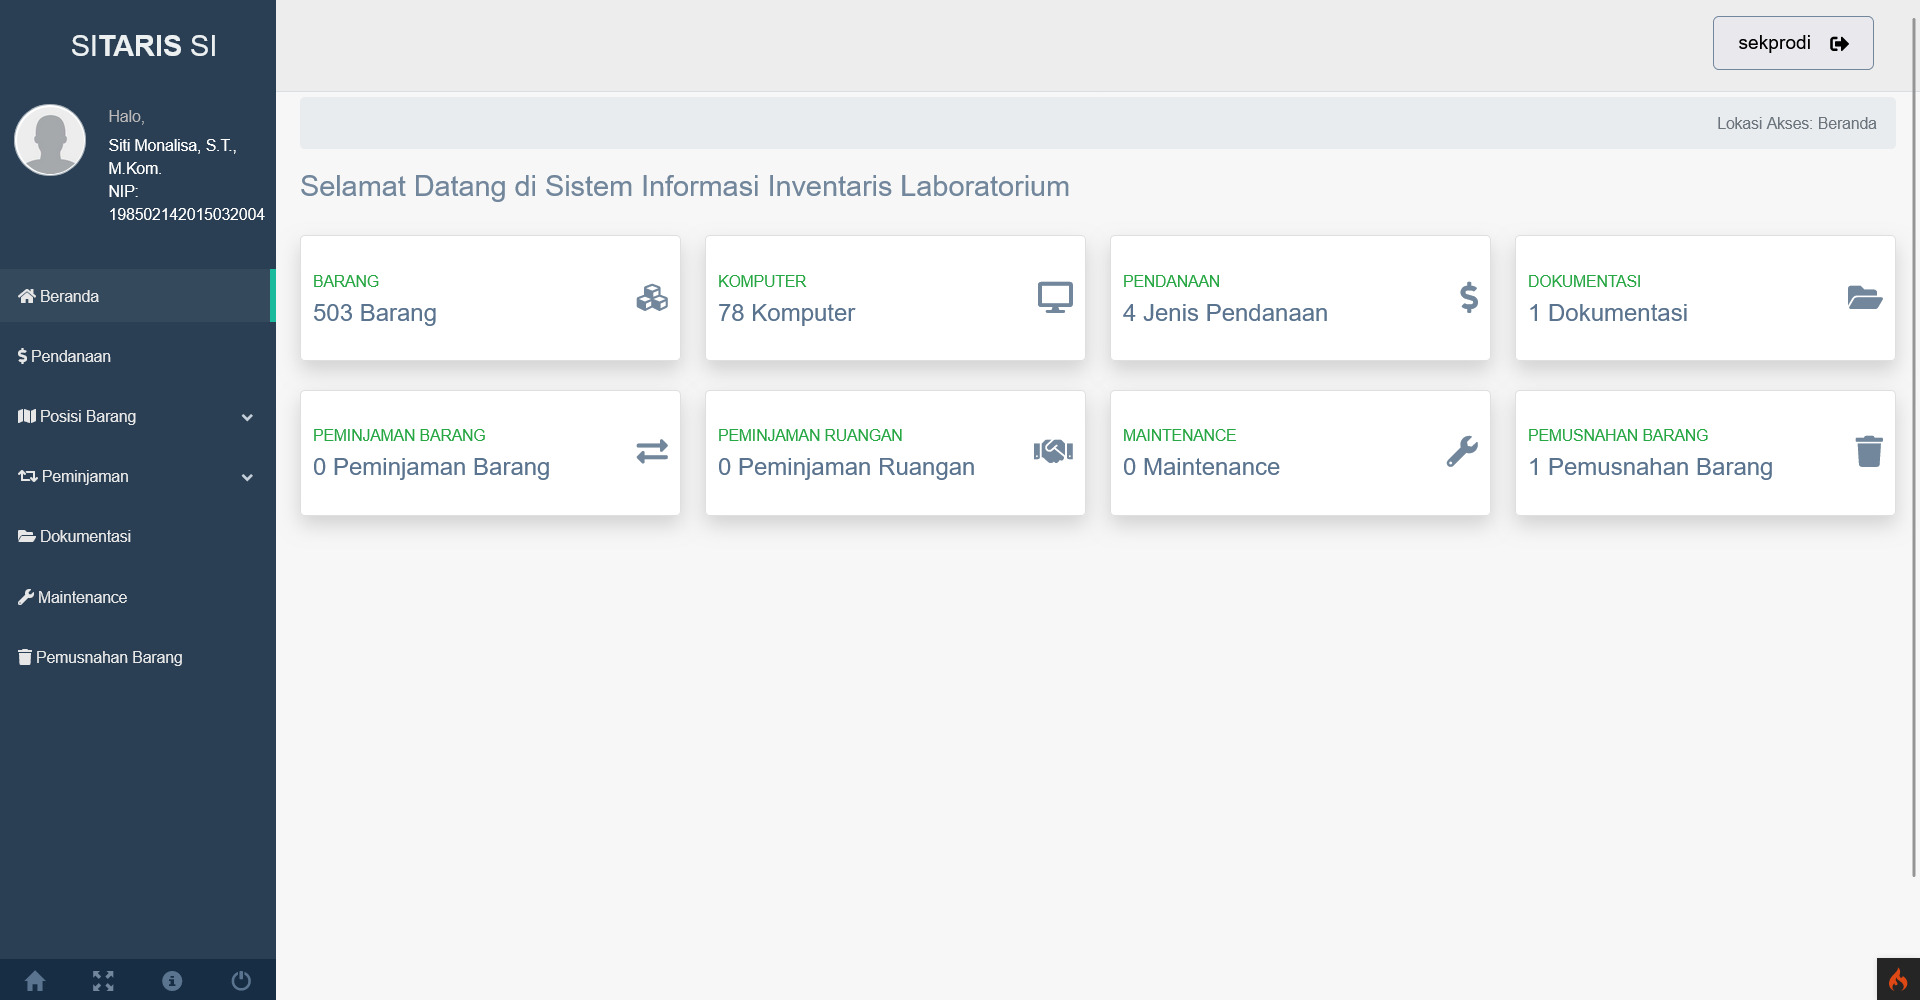
\includegraphics[width=0.82\linewidth]{konten//gambar/sekprodi.png}
        %   \caption{Halaman Beranda Sekprodi}
        %   \label{fig:enter-label}
        % \end{figure}

        % \begin{figure}
        %   \centering
        %   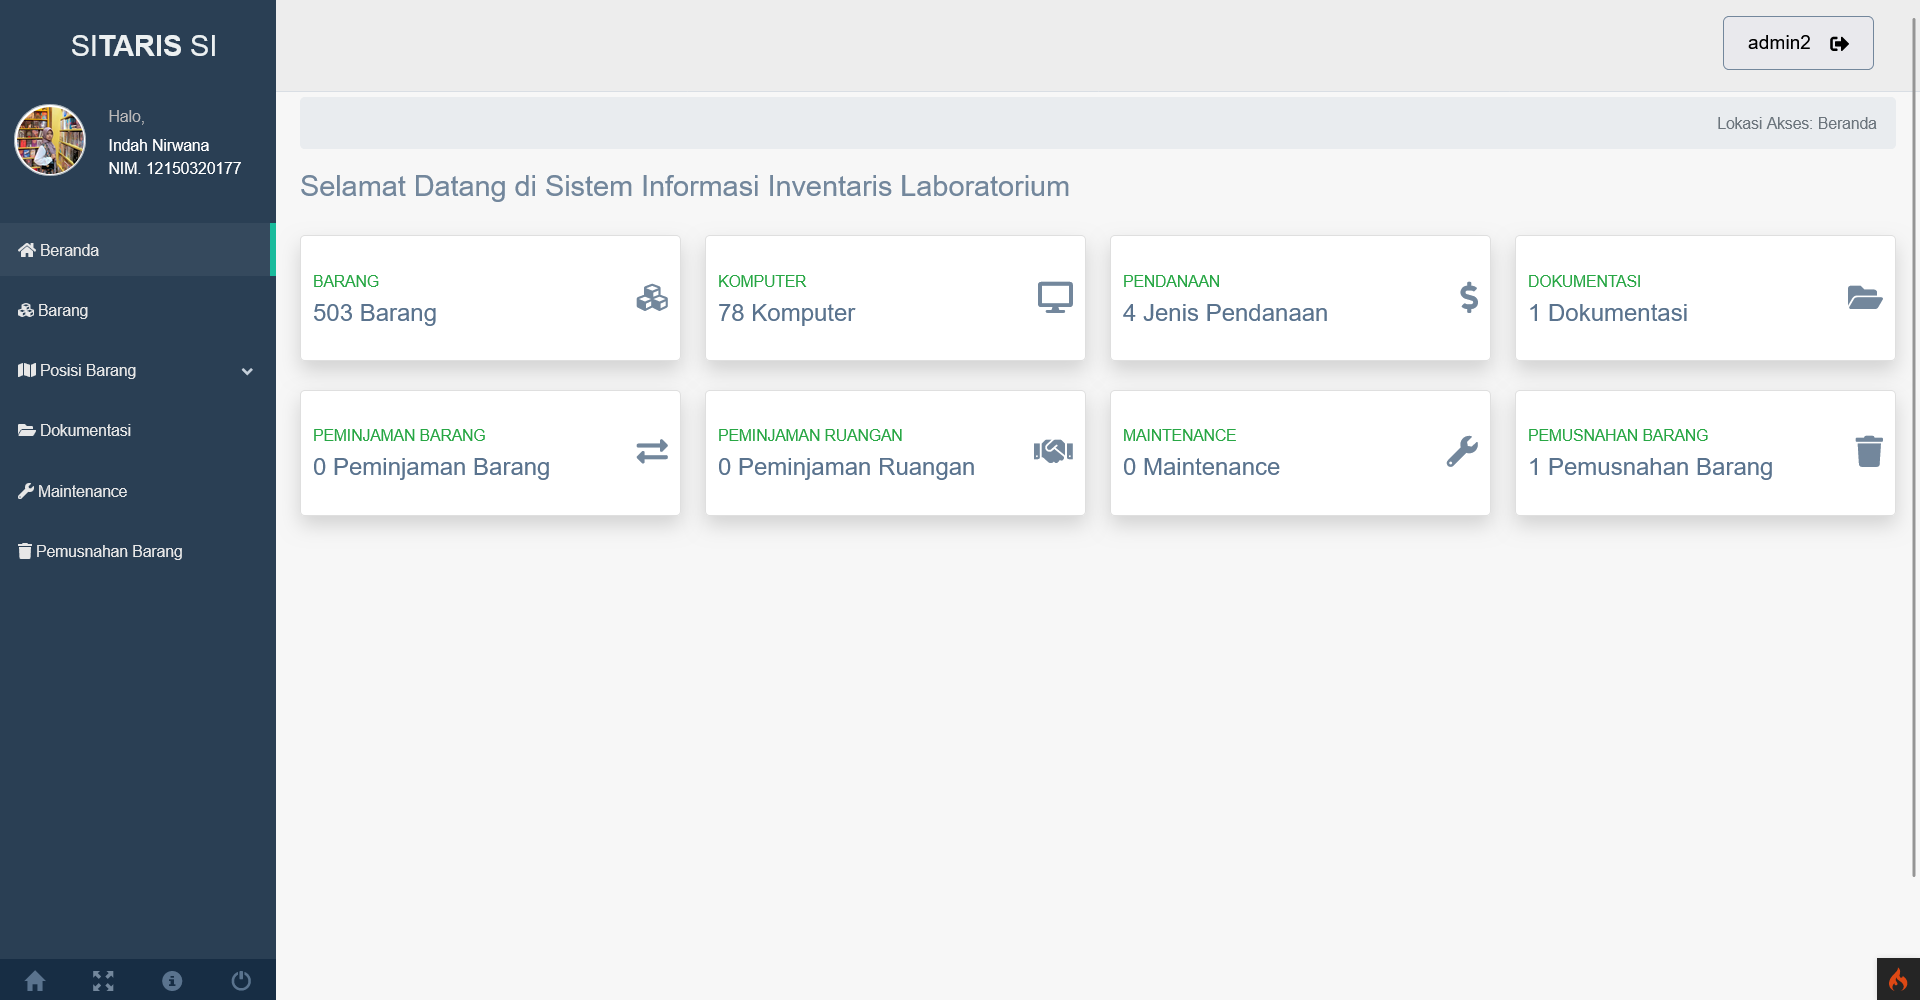
\includegraphics[width=0.82\linewidth]{konten//gambar/aslab.png}
        %   \caption{Halaman Beranda Aslab}
        %   \label{fig:enter-label}
        % \end{figure}

  \item Halaman Pendanaan \\ Halaman pendanaan merupakan tampilan untuk melihat dan mengelola data pendanaan, tombol tambah data merupakan tombol yang dapat digunakan untuk beralih ke halaman tambah data pendanaan, dan tombol pensil digunakan untuk mengedit data pendanaan dan tombol \textit{trash} untuk menghapus data pendanaan seperti pada Gambar 2.4. sampai Gambar 2.6.

        \begin{figure}
          \centering
          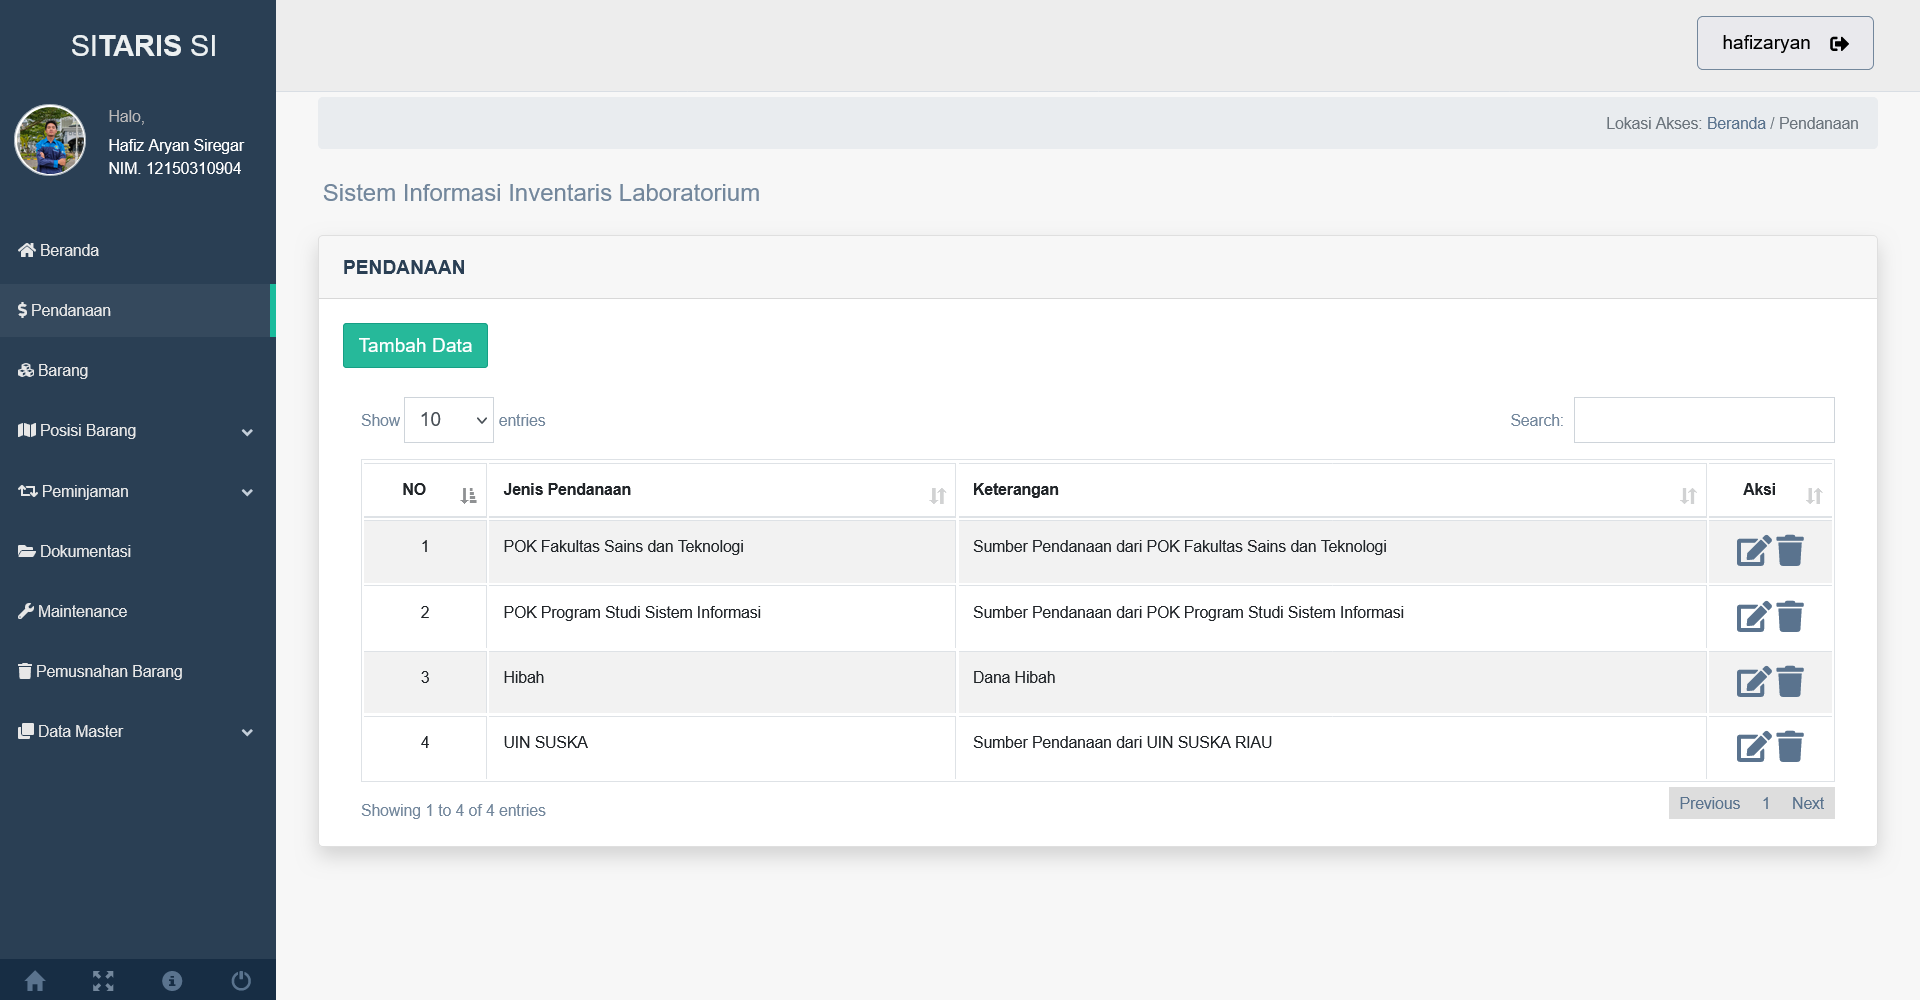
\includegraphics[width=0.82\linewidth]{konten//gambar/pendanaan.png}
          \caption{Halaman Pendanaan \textit{Index}}
          \label{fig:enter-label}
        \end{figure}

        \begin{figure}
          \centering
          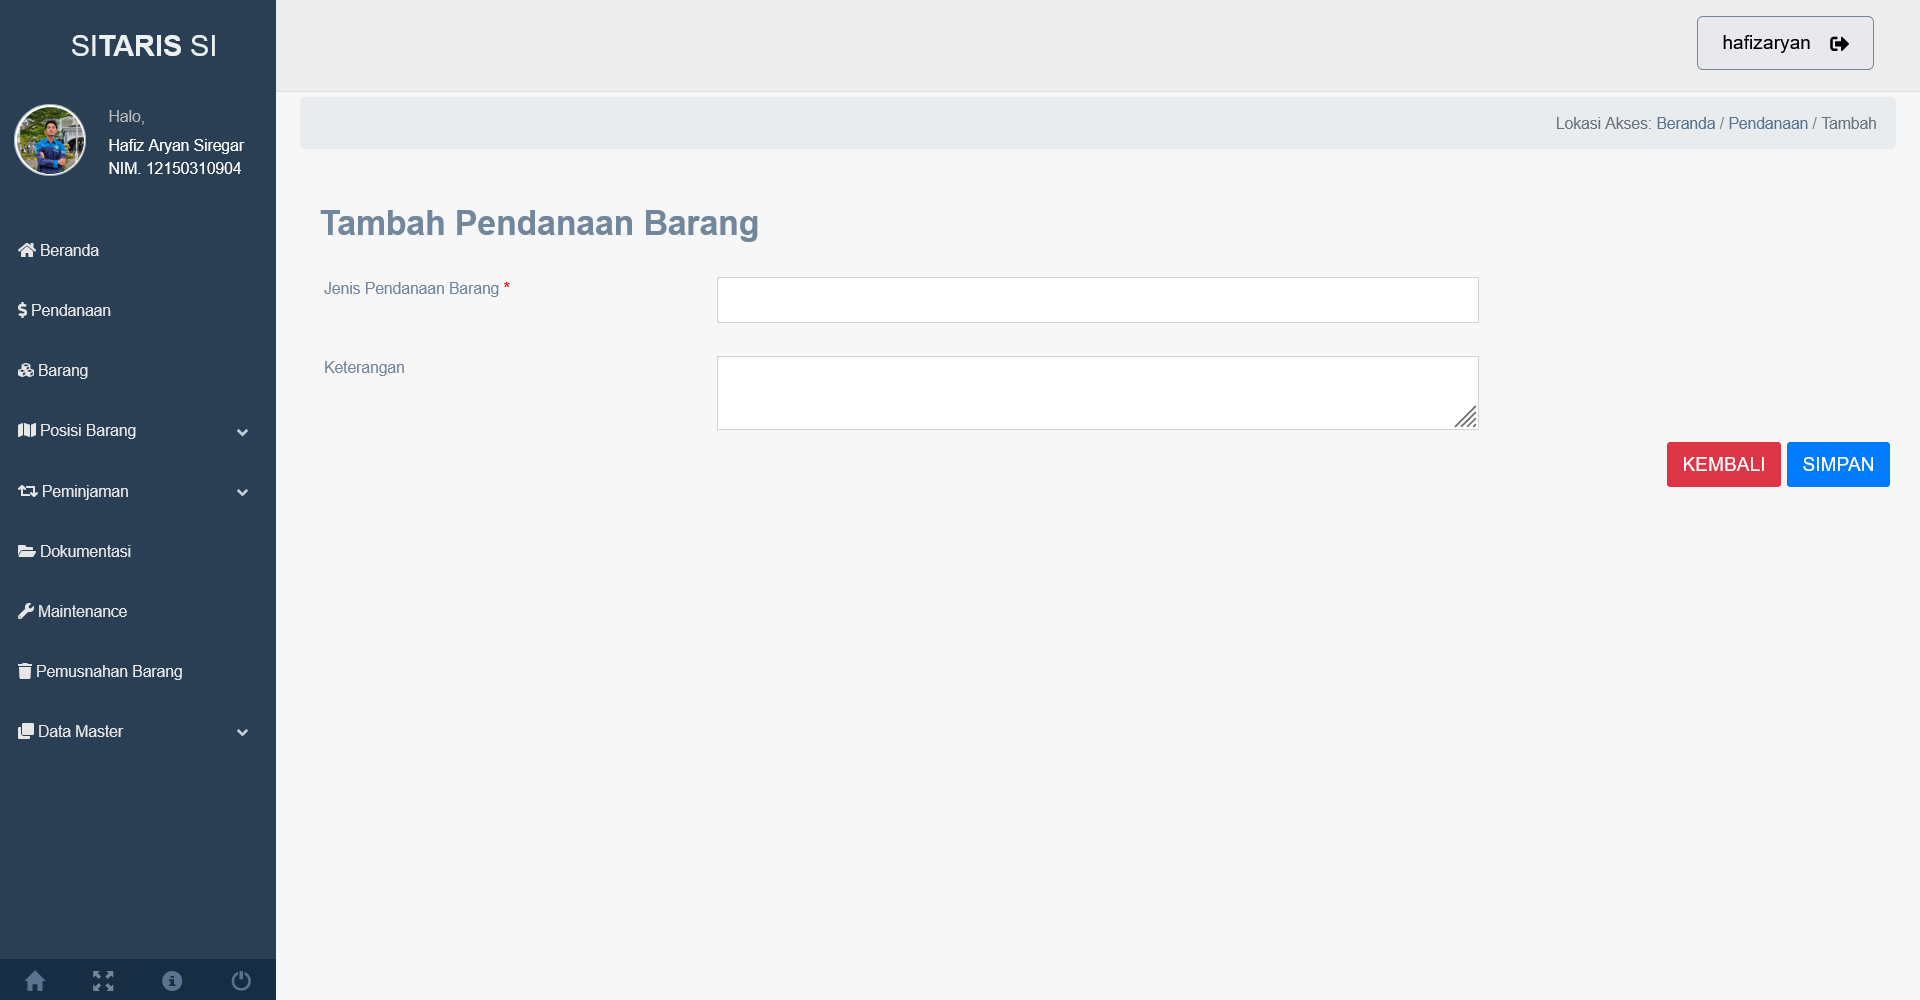
\includegraphics[width=0.82\linewidth]{konten//gambar/pendanaan tambah.png}
          \caption{Halaman Tambah Pendanaan}
          \label{fig:enter-label}
        \end{figure}

        \begin{figure}
          \centering
          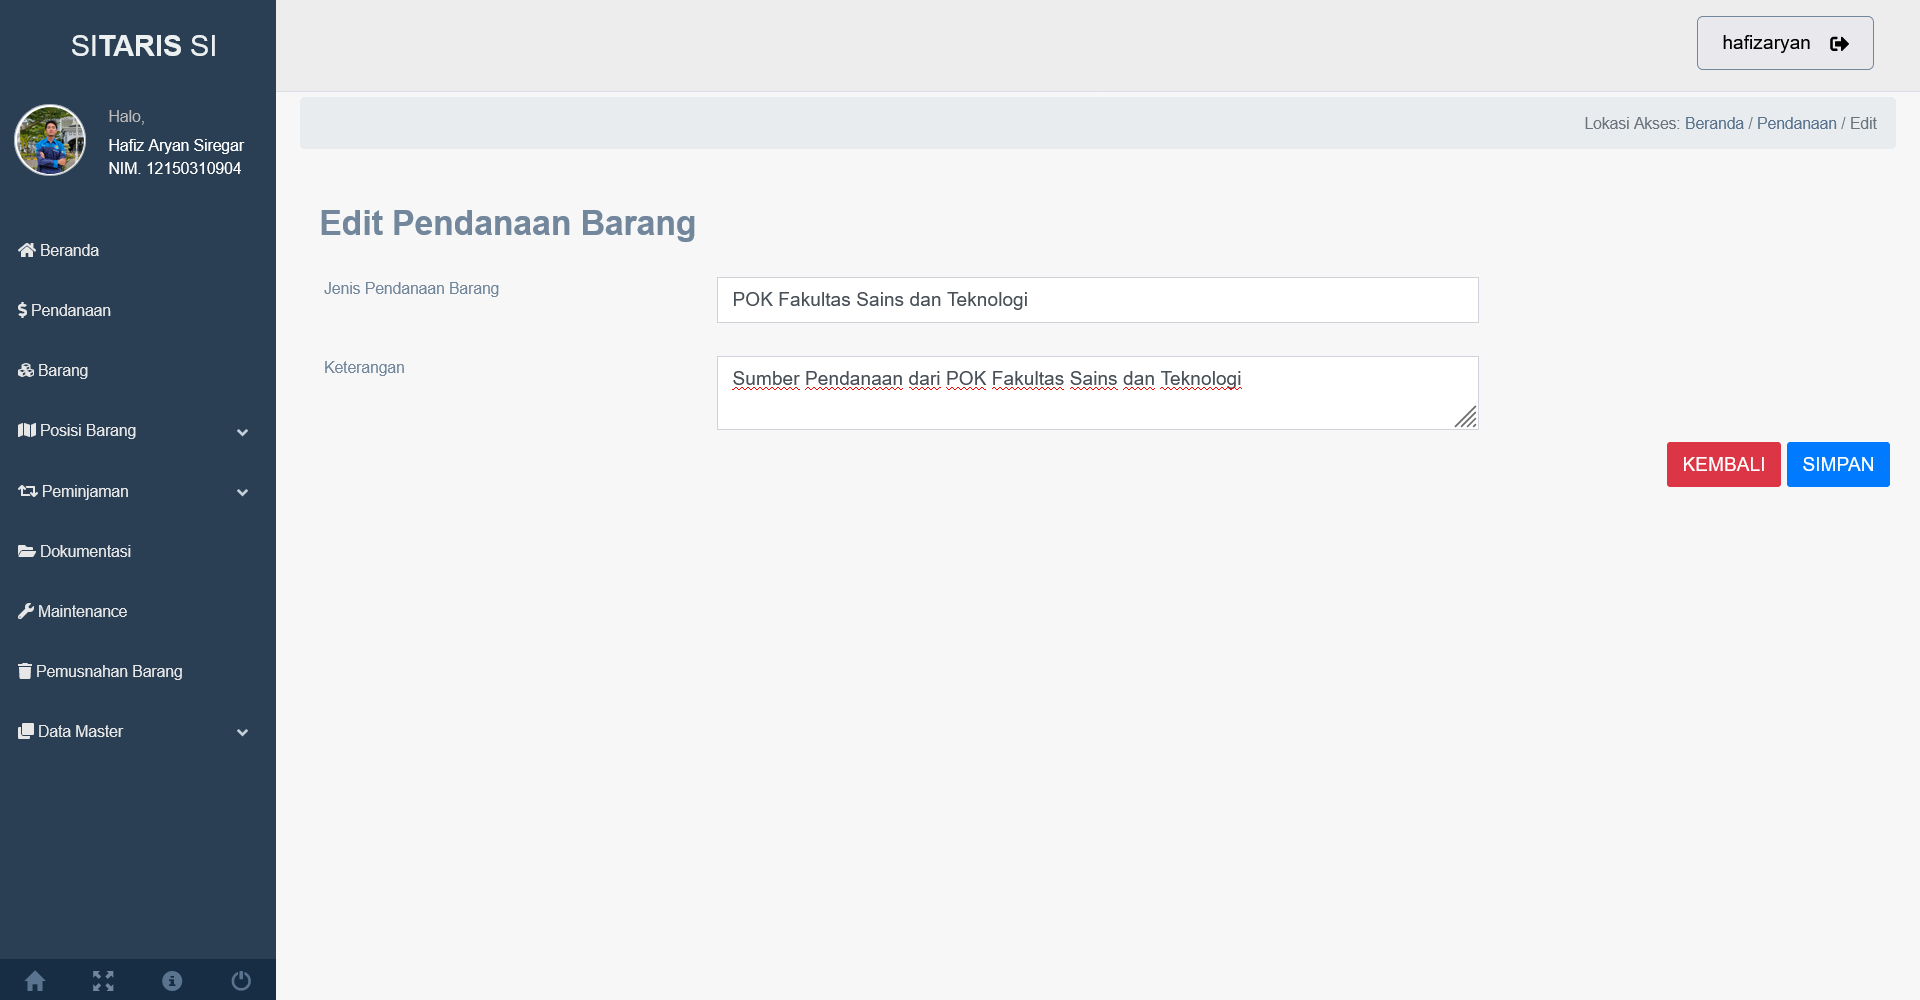
\includegraphics[width=0.82\linewidth]{konten//gambar/pendanaan edit.png}
          \caption{Halaman Edit Pendanaan}
          \label{fig:enter-label}
        \end{figure}

  \item Halaman Barang \\ Halaman barang merupakan tampilan untuk melihat dan mengelola data barang, tombol tambah data merupakan tombol yang dapat digunakan untuk beralih ke halaman tambah data barang, dan tombol pensil digunakan untuk mengedit data barang dan tombol \textit{trash} untuk menghapus data barang, lalu terdapat juga tombol berwarna biru toska yang dibedakan menjadi beberapa tombol yang bertujuan untuk mencetak dokumen laporan berdasarkan pendanaan, ruangan, kategori, tahun, dan QR seperti pada Gambar 2.7. sampai Gambar 2.19.

        \begin{figure}
          \centering
          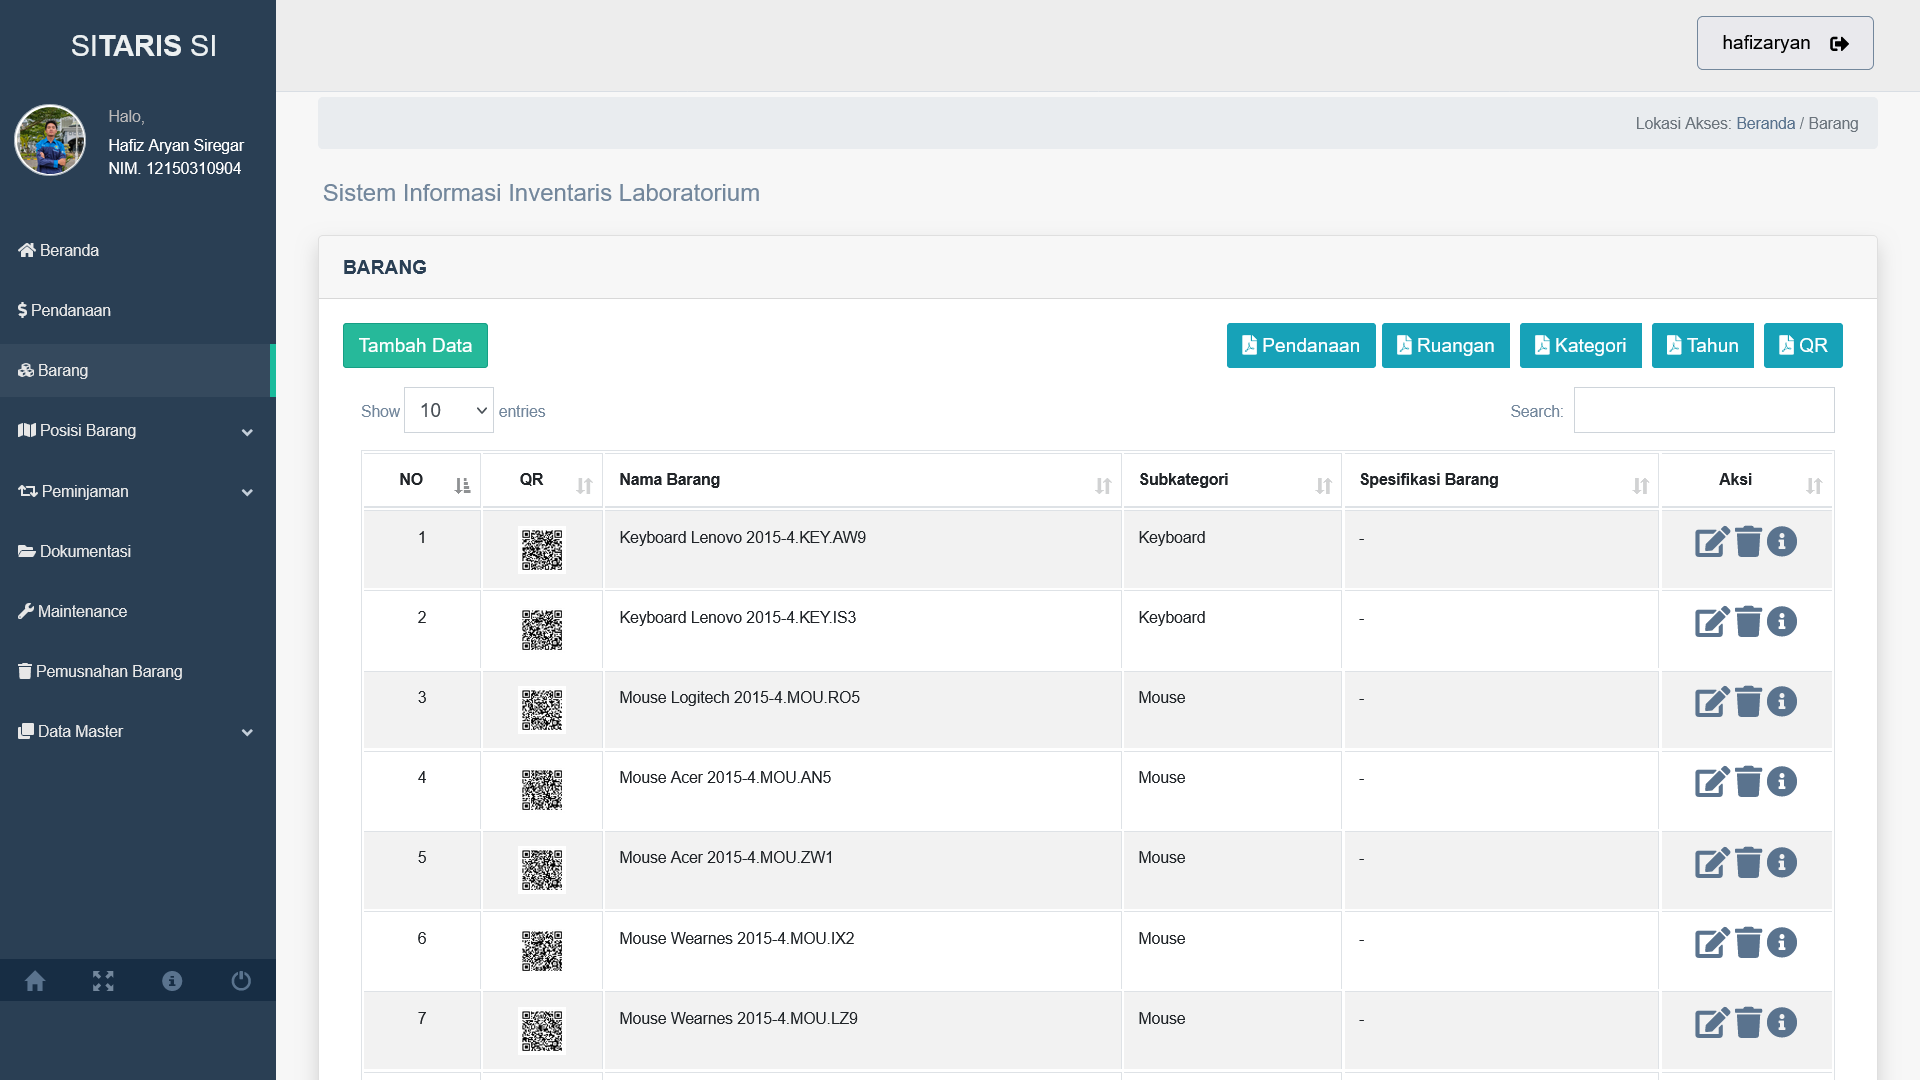
\includegraphics[width=0.82\linewidth]{konten//gambar/barang.png}
          \caption{Halaman Barang \textit{Index}}
          \label{fig:enter-label}
        \end{figure}

        \begin{figure}
          \centering
          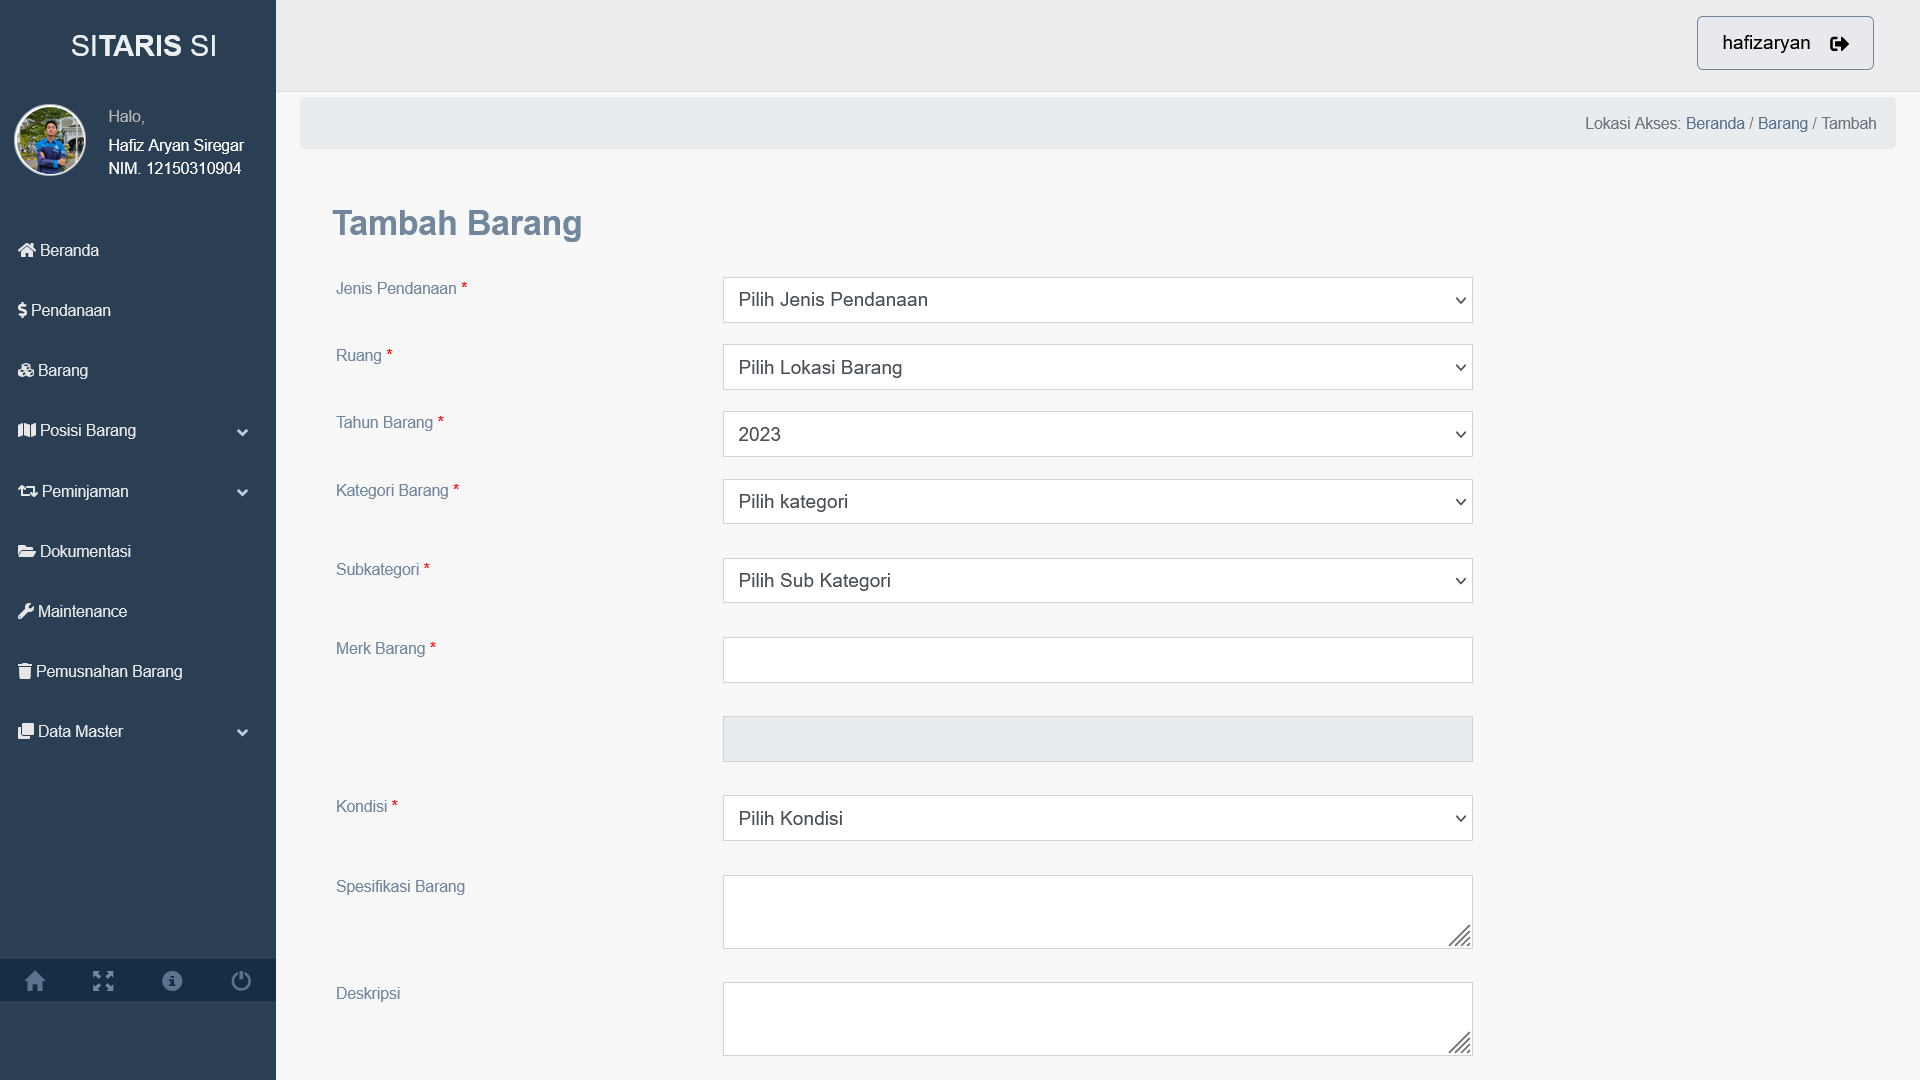
\includegraphics[width=0.82\linewidth]{konten//gambar/barang tambah.png}
          \caption{Halaman Tambah Barang}
          \label{fig:enter-label}
        \end{figure}

        \begin{figure}
          \centering
          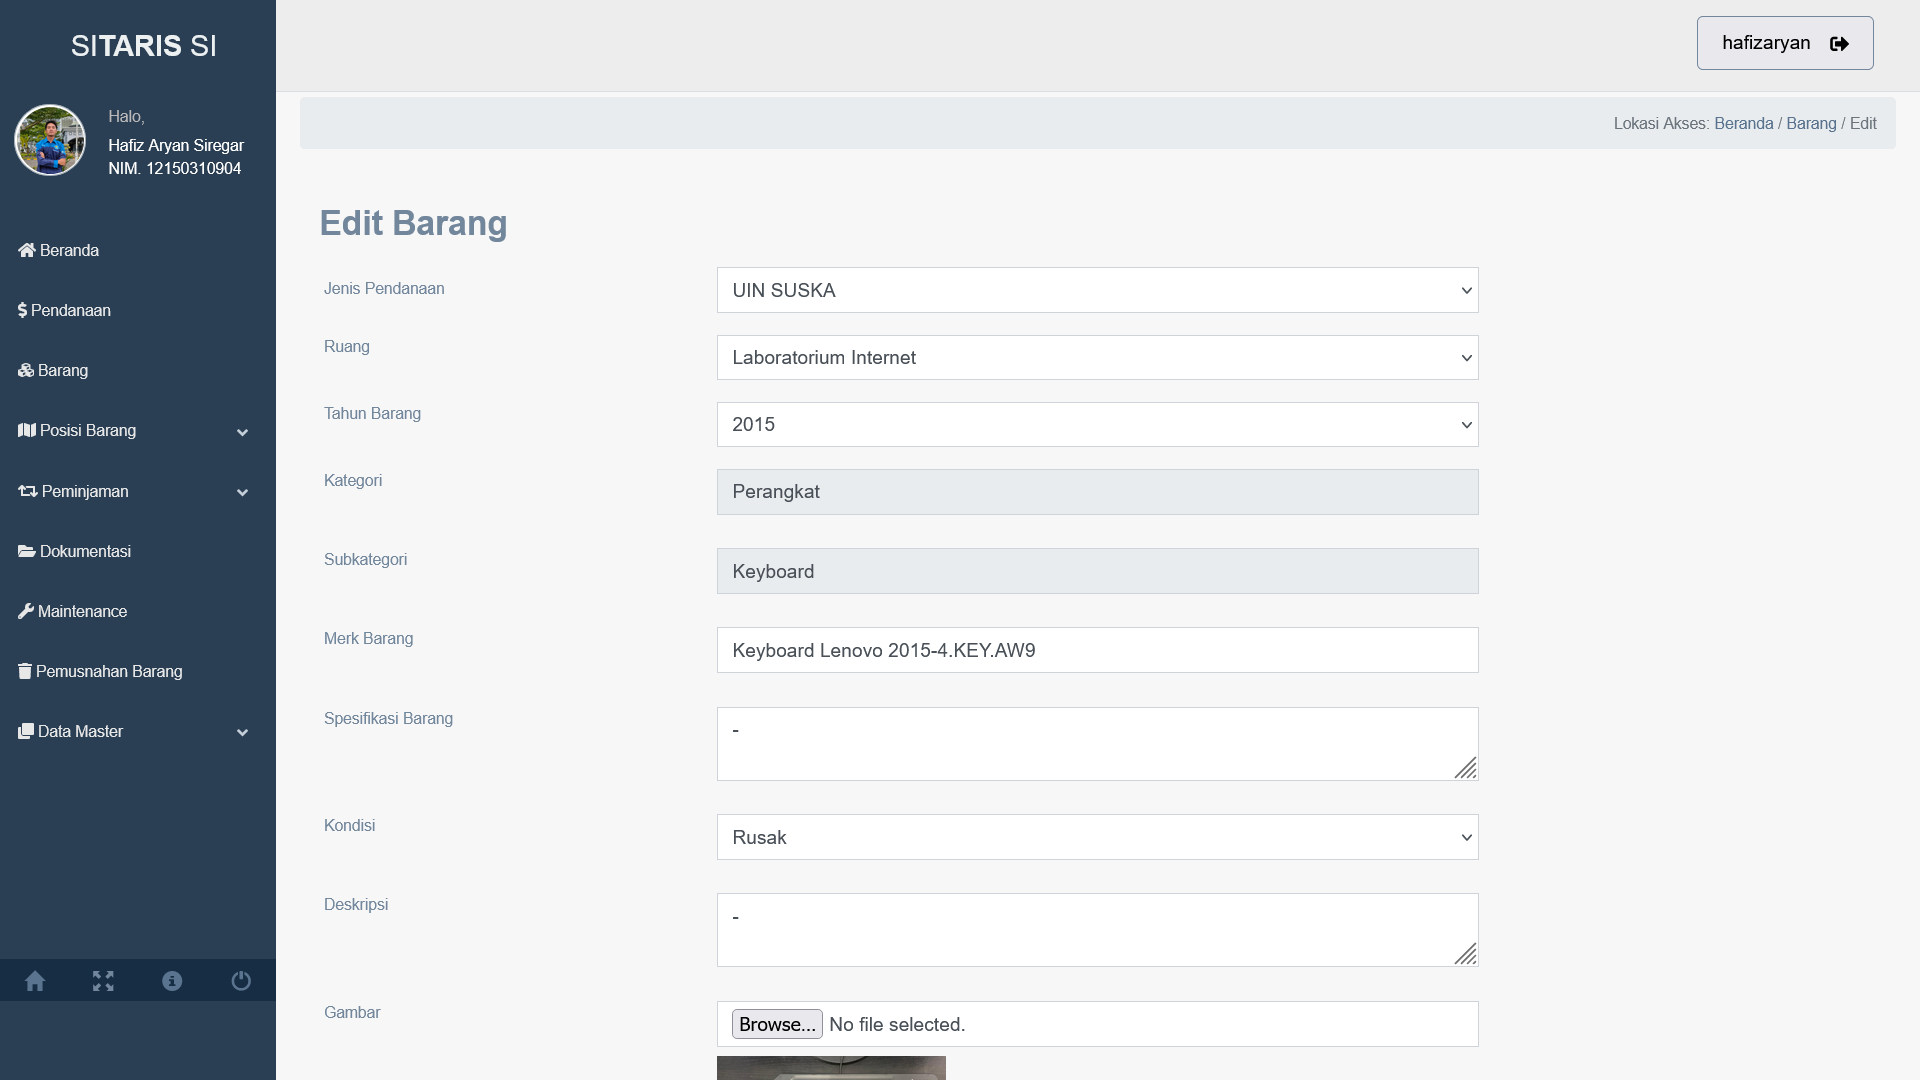
\includegraphics[width=0.82\linewidth]{konten//gambar/barang edit.png}
          \caption{Halaman Edit Barang}
          \label{fig:enter-label}
        \end{figure}

        \begin{figure}
          \centering
          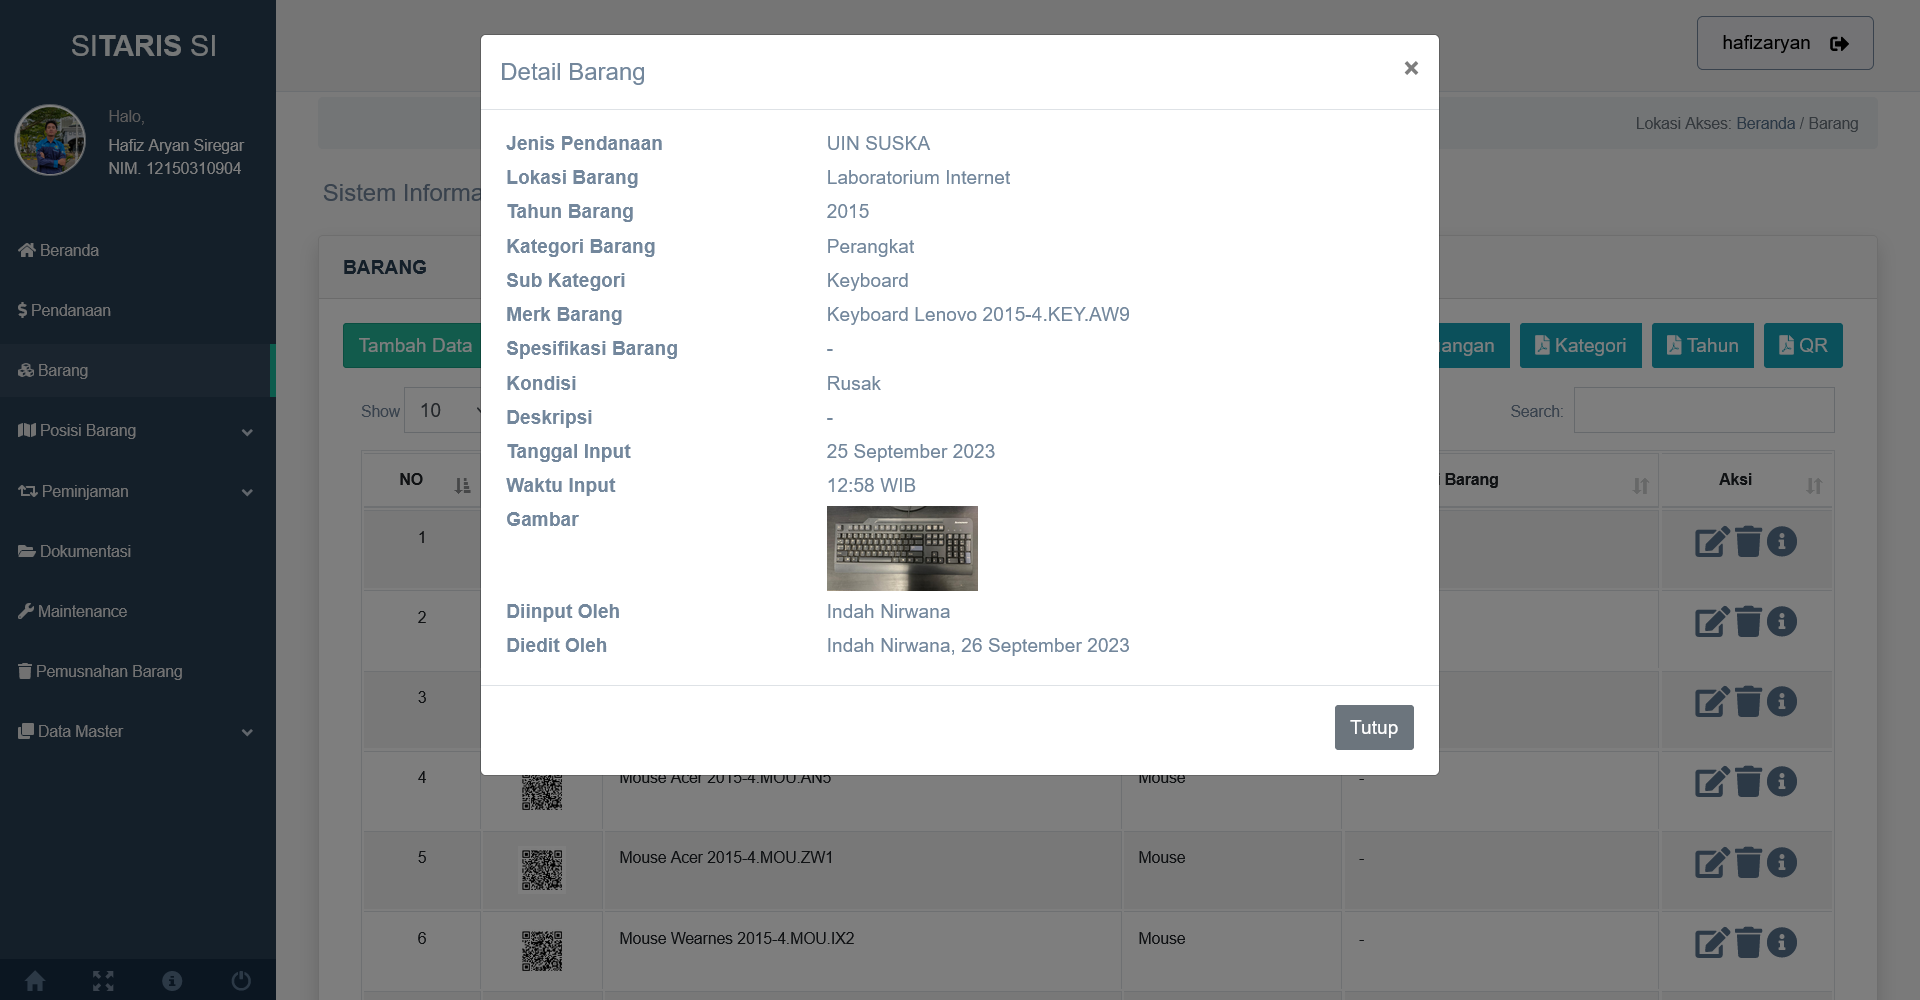
\includegraphics[width=0.82\linewidth]{konten//gambar/barang detail.png}
          \caption{Tampilan Detail Barang}
          \label{fig:enter-label}
        \end{figure}

        \begin{figure}
          \centering
          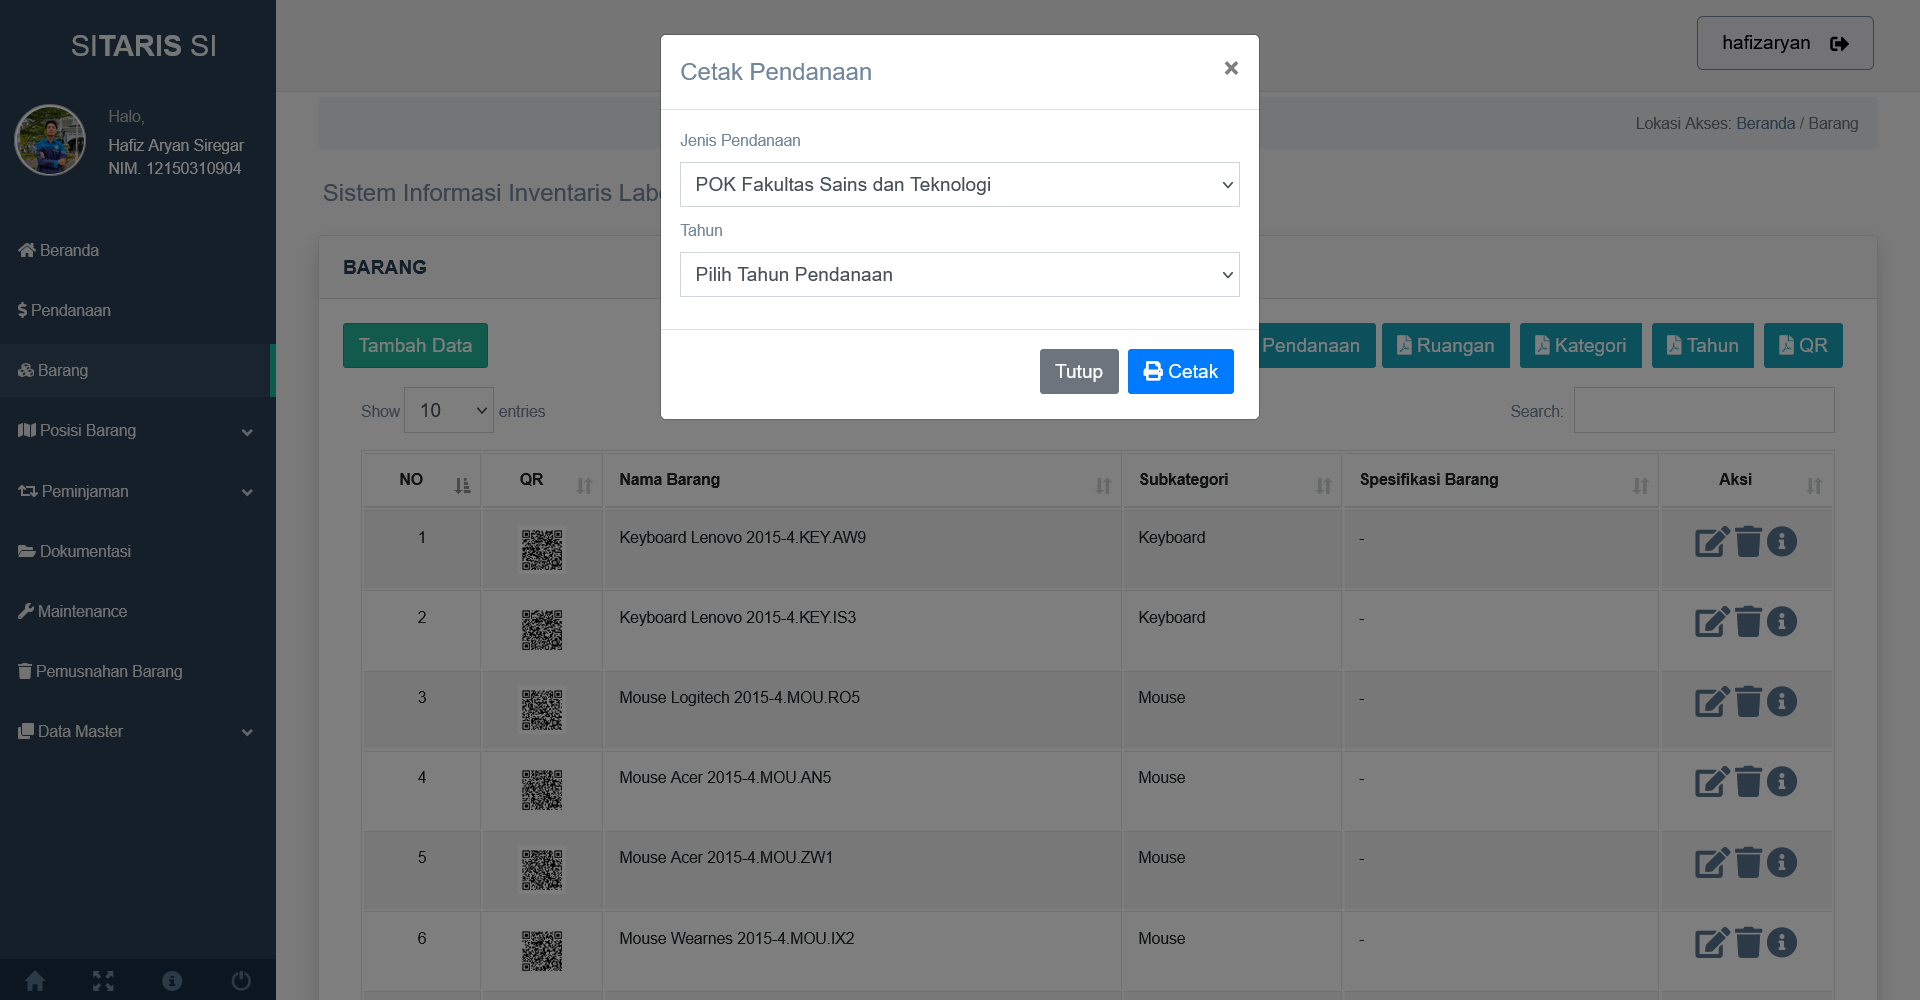
\includegraphics[width=0.82\linewidth]{konten//gambar/barang cetak pendanaan.png}
          \caption{Tampilan Tombol Cetak Pendanaan}
          \label{fig:enter-label}
        \end{figure}

        \begin{figure}
          \centering
          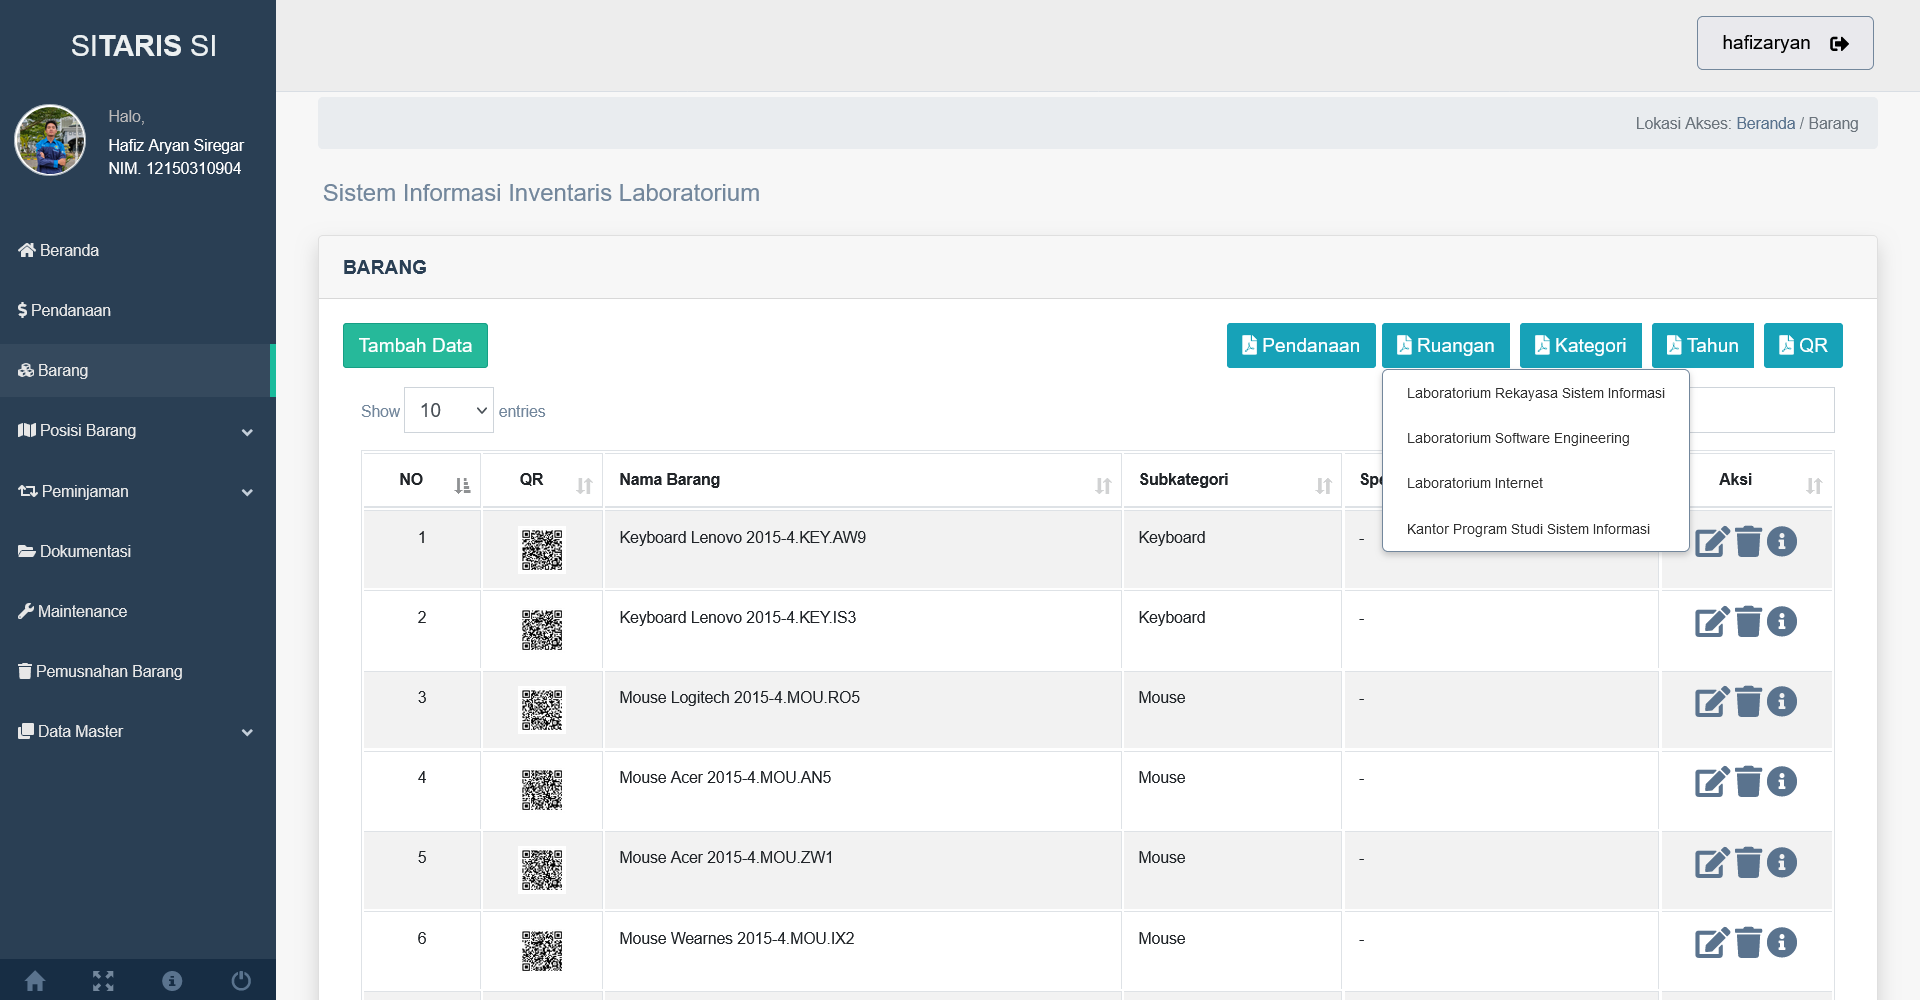
\includegraphics[width=0.82\linewidth]{konten//gambar/barang cetak ruangan.png}
          \caption{Tampilan Tombol Cetak Ruangan}
          \label{fig:enter-label}
        \end{figure}

        \begin{figure}
          \centering
          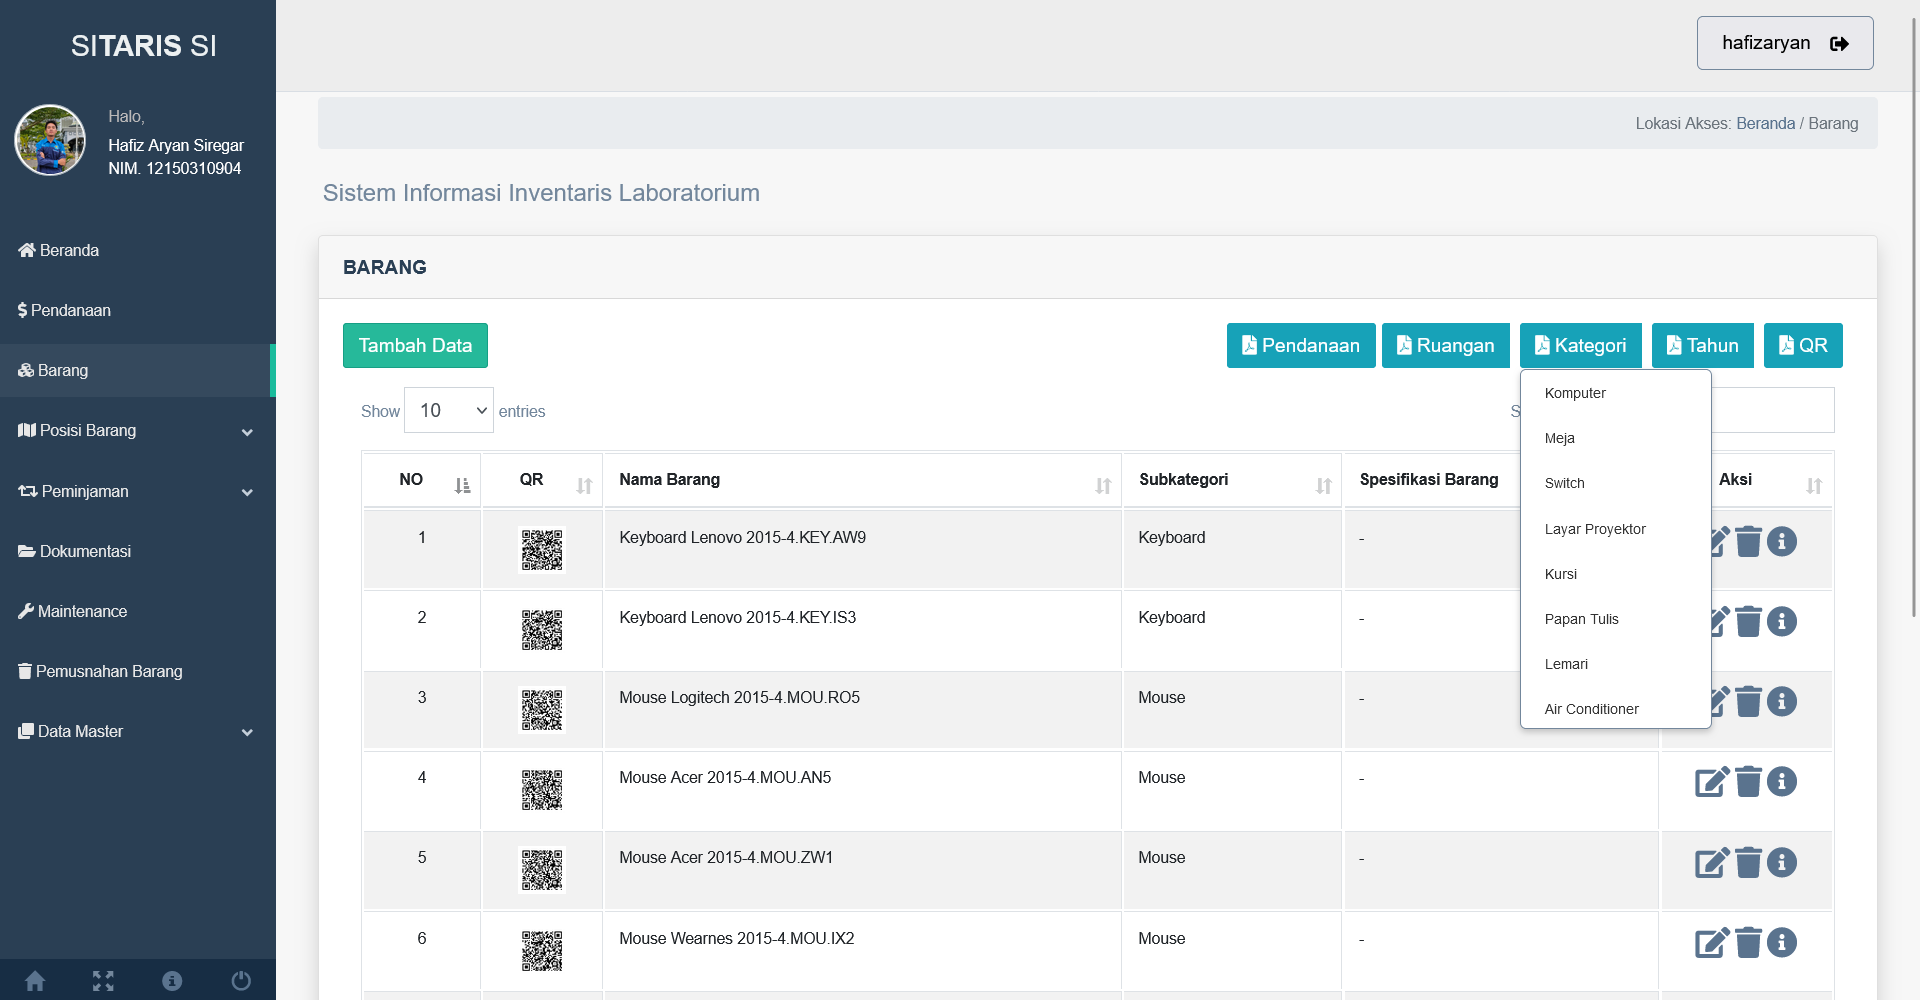
\includegraphics[width=0.82\linewidth]{konten//gambar/barang cetak kategori.png}
          \caption{Tampilan Tombol Cetak Kategori}
          \label{fig:enter-label}
        \end{figure}

        \begin{figure}
          \centering
          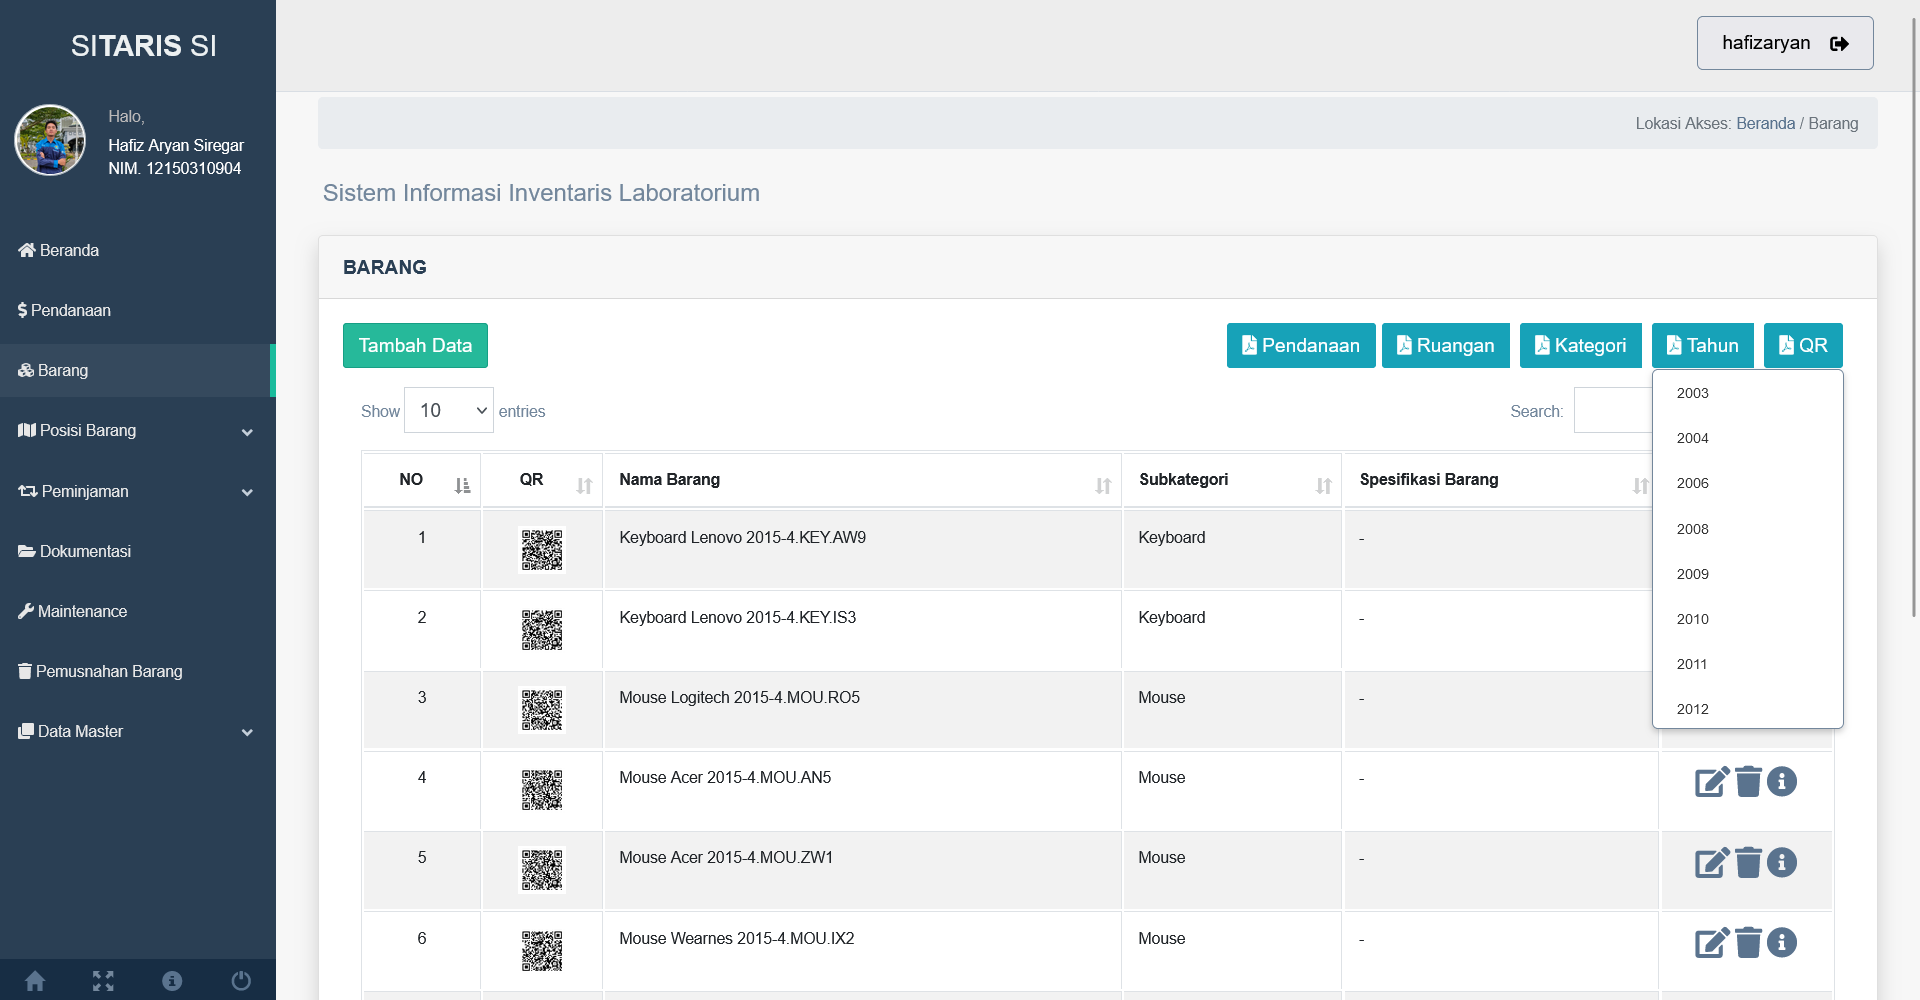
\includegraphics[width=0.82\linewidth]{konten//gambar/barang cetak tahun.png}
          \caption{Tampilan Tombol Cetak Tahun}
          \label{fig:enter-label}
        \end{figure}

        \begin{figure}
          \centering
          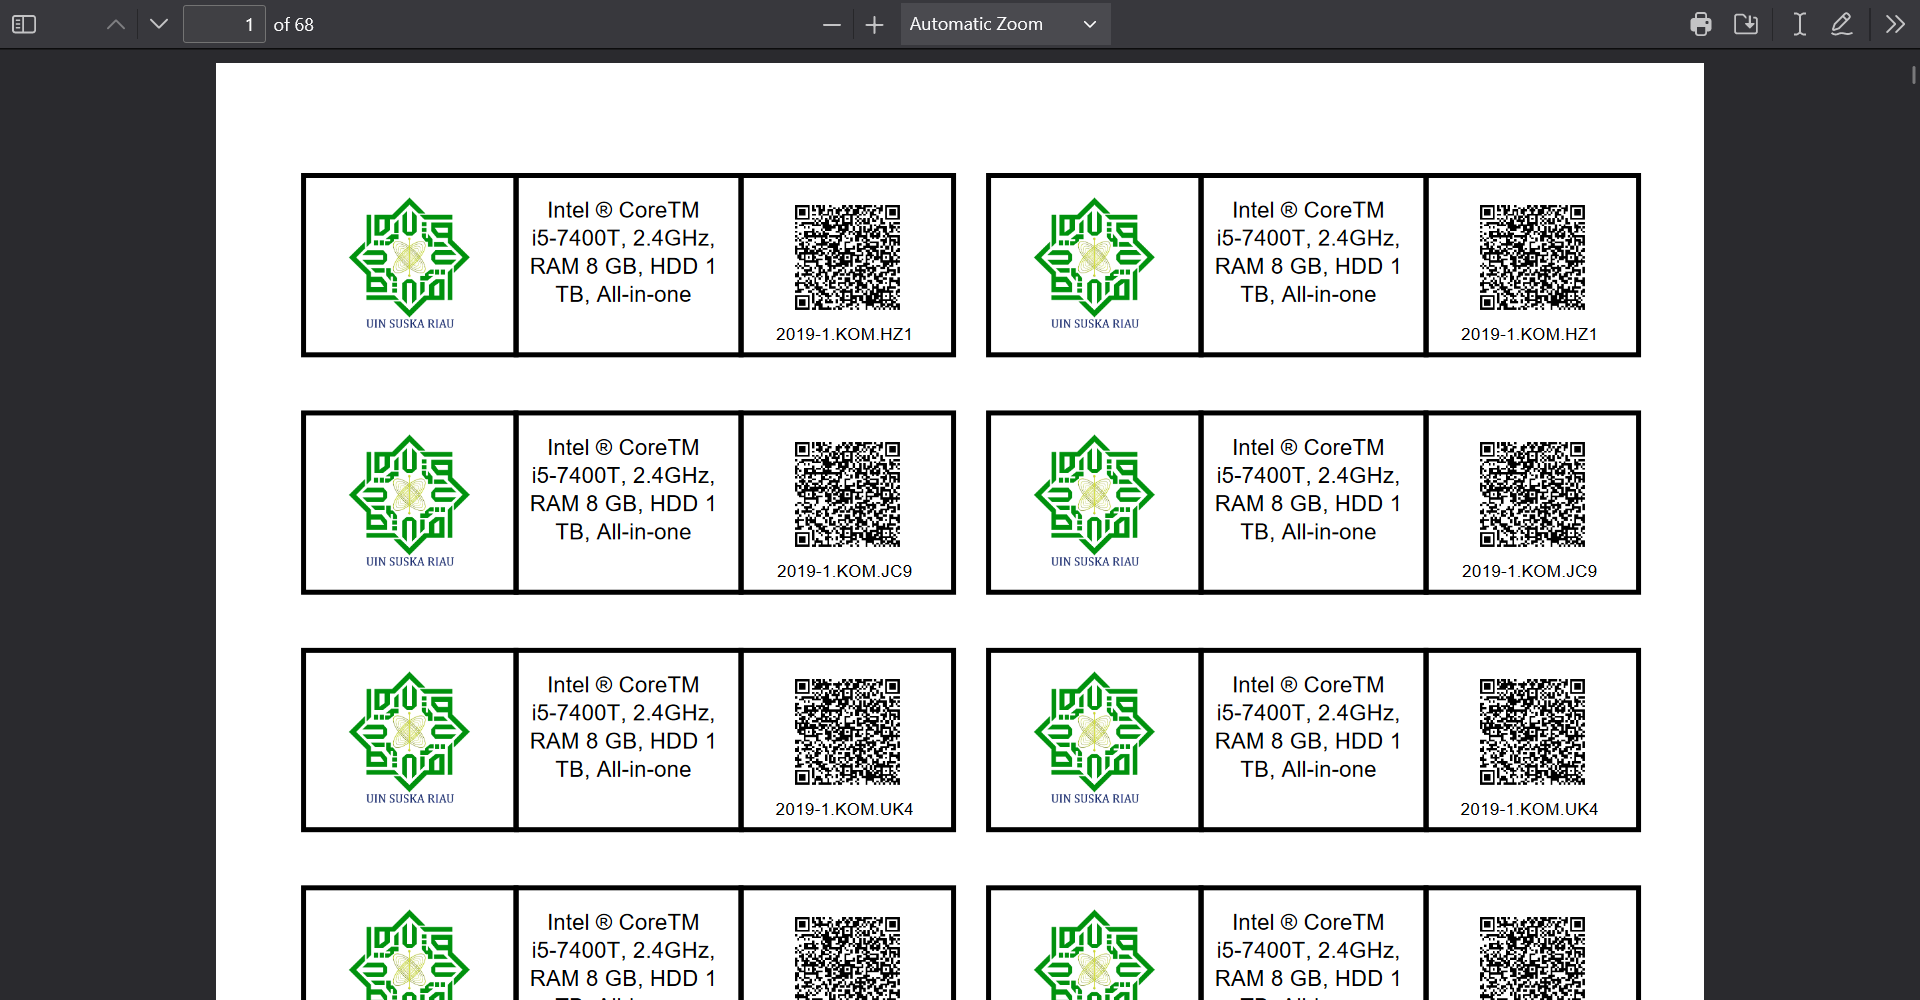
\includegraphics[width=0.82\linewidth]{konten//gambar/barang cetak qr.png}
          \caption{Halaman Cetak QR}
          \label{fig:enter-label}
        \end{figure}

        \begin{figure}
          \centering
          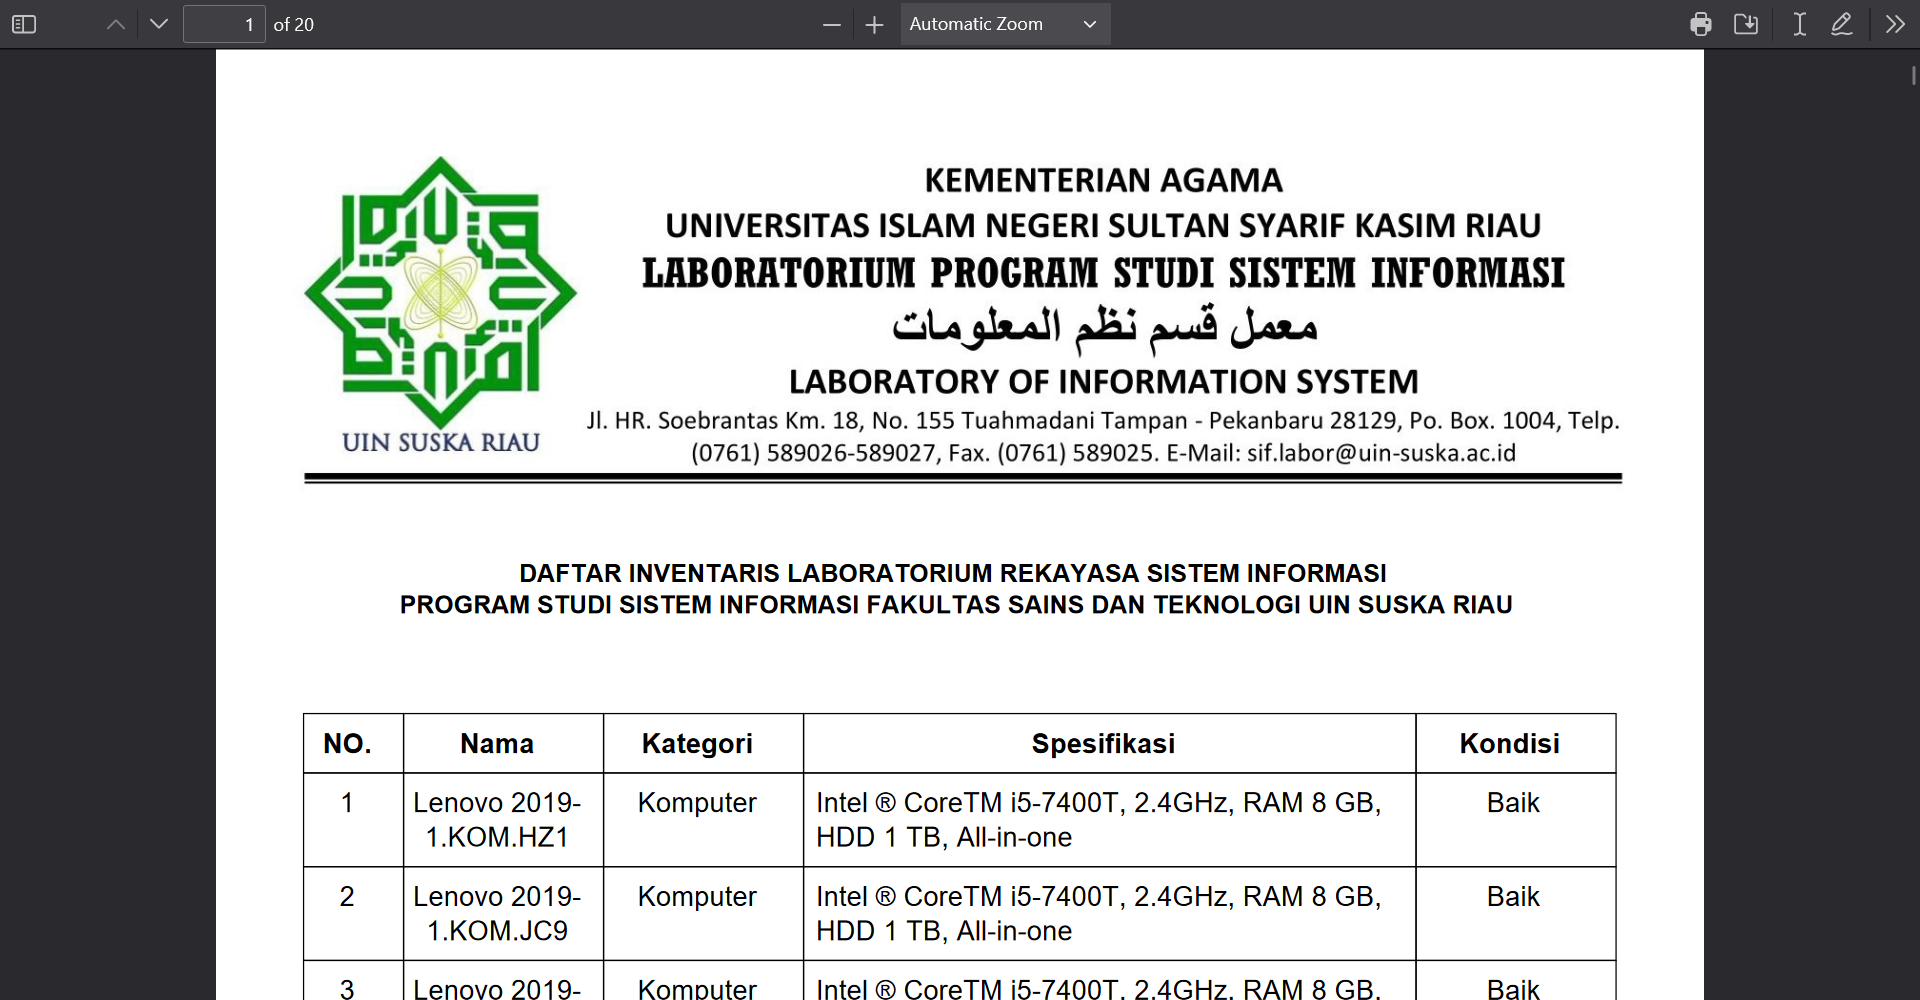
\includegraphics[width=0.82\linewidth]{konten//gambar/barang cetak ruangan pdf.png}
          \caption{Halaman Cetak Ruangan}
          \label{fig:enter-label}
        \end{figure}

        \begin{figure}
          \centering
          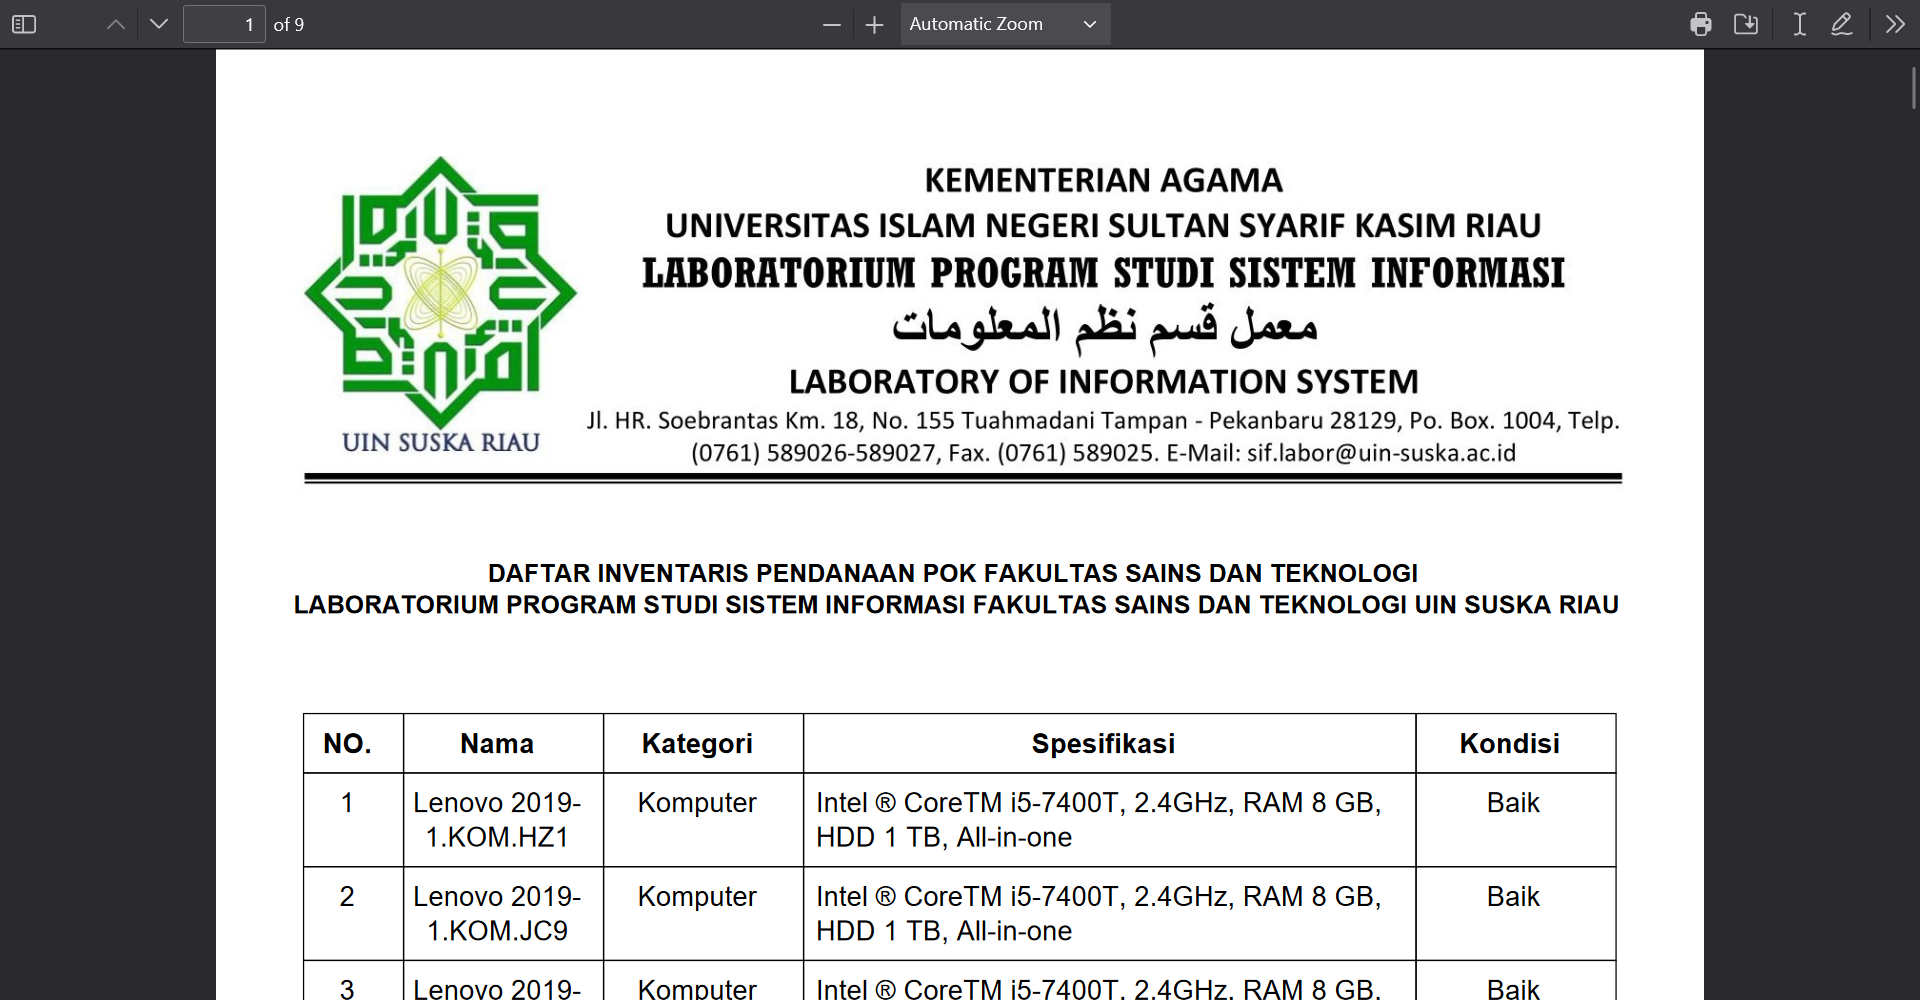
\includegraphics[width=0.82\linewidth]{konten//gambar/barang cetak pendanaan pdf.png}
          \caption{Halaman Cetak Pendanaan}
          \label{fig:enter-label}
        \end{figure}

        \begin{figure}
          \centering
          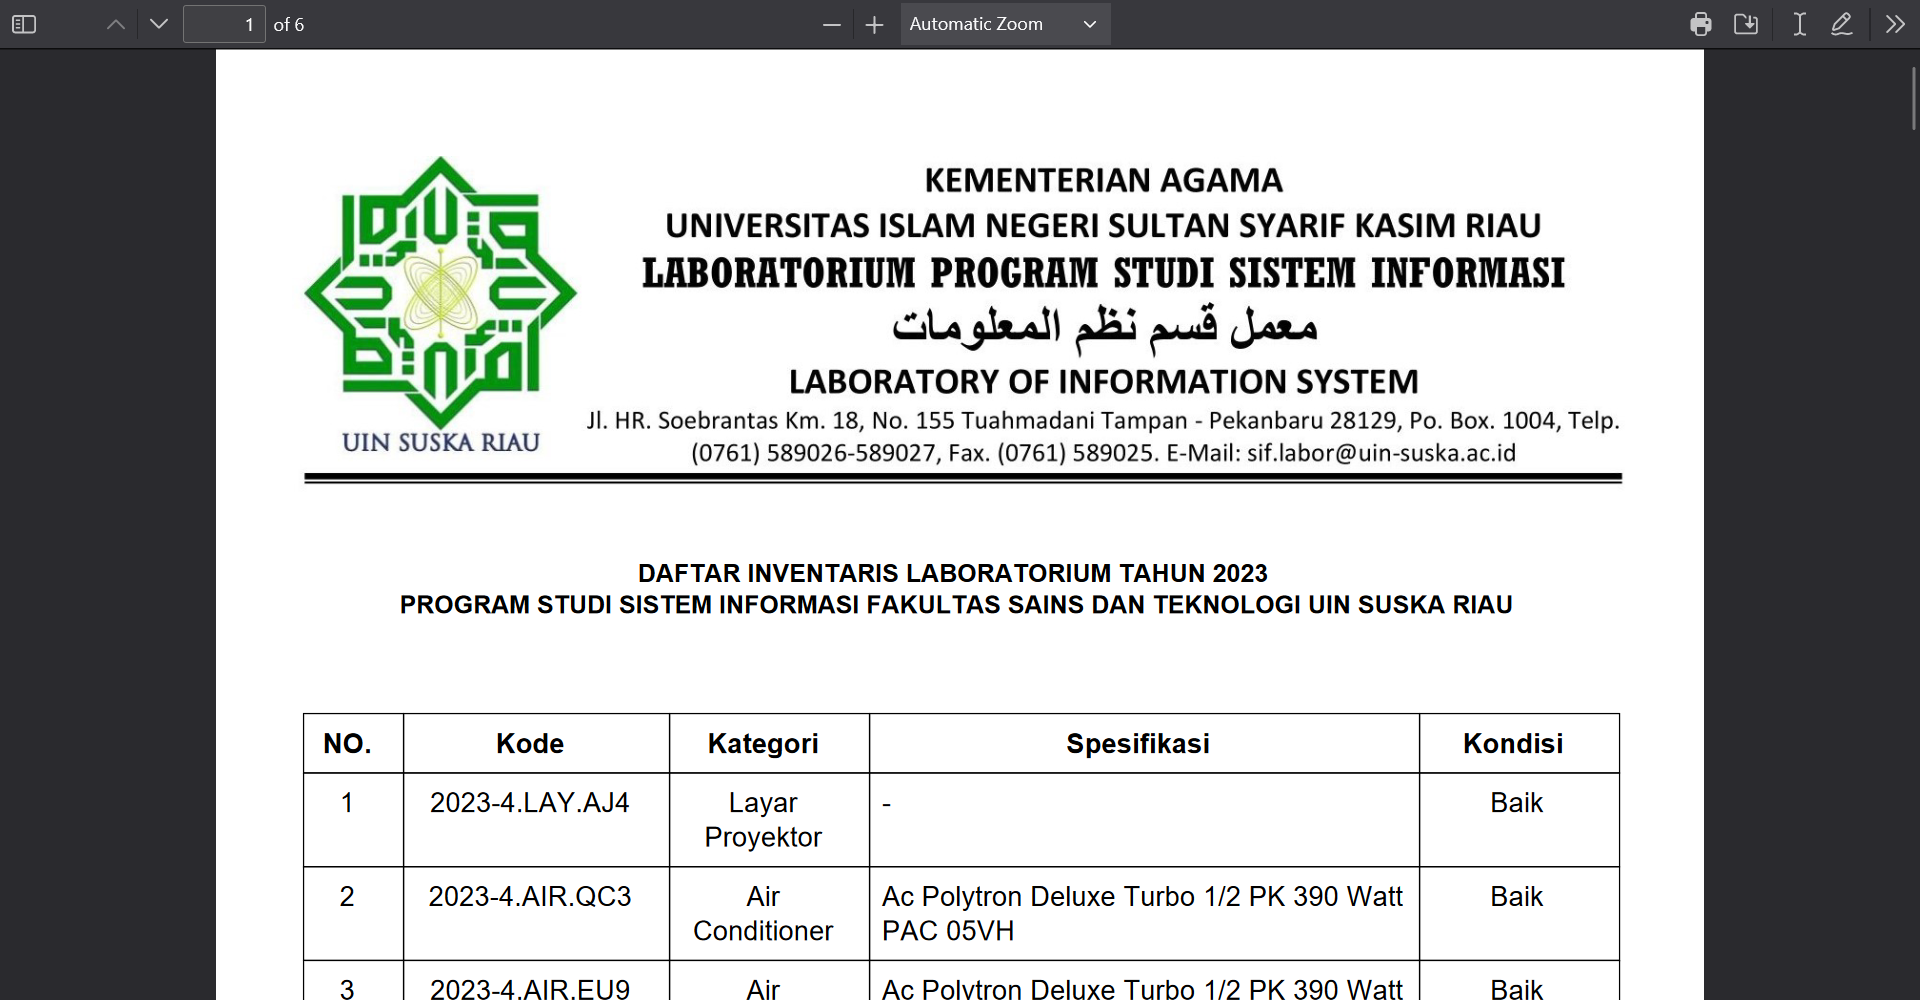
\includegraphics[width=0.82\linewidth]{konten//gambar/barang cetak tahun pdf.png}
          \caption{Halaman Cetak Tahun}
          \label{fig:enter-label}
        \end{figure}

        \begin{figure}
          \centering
          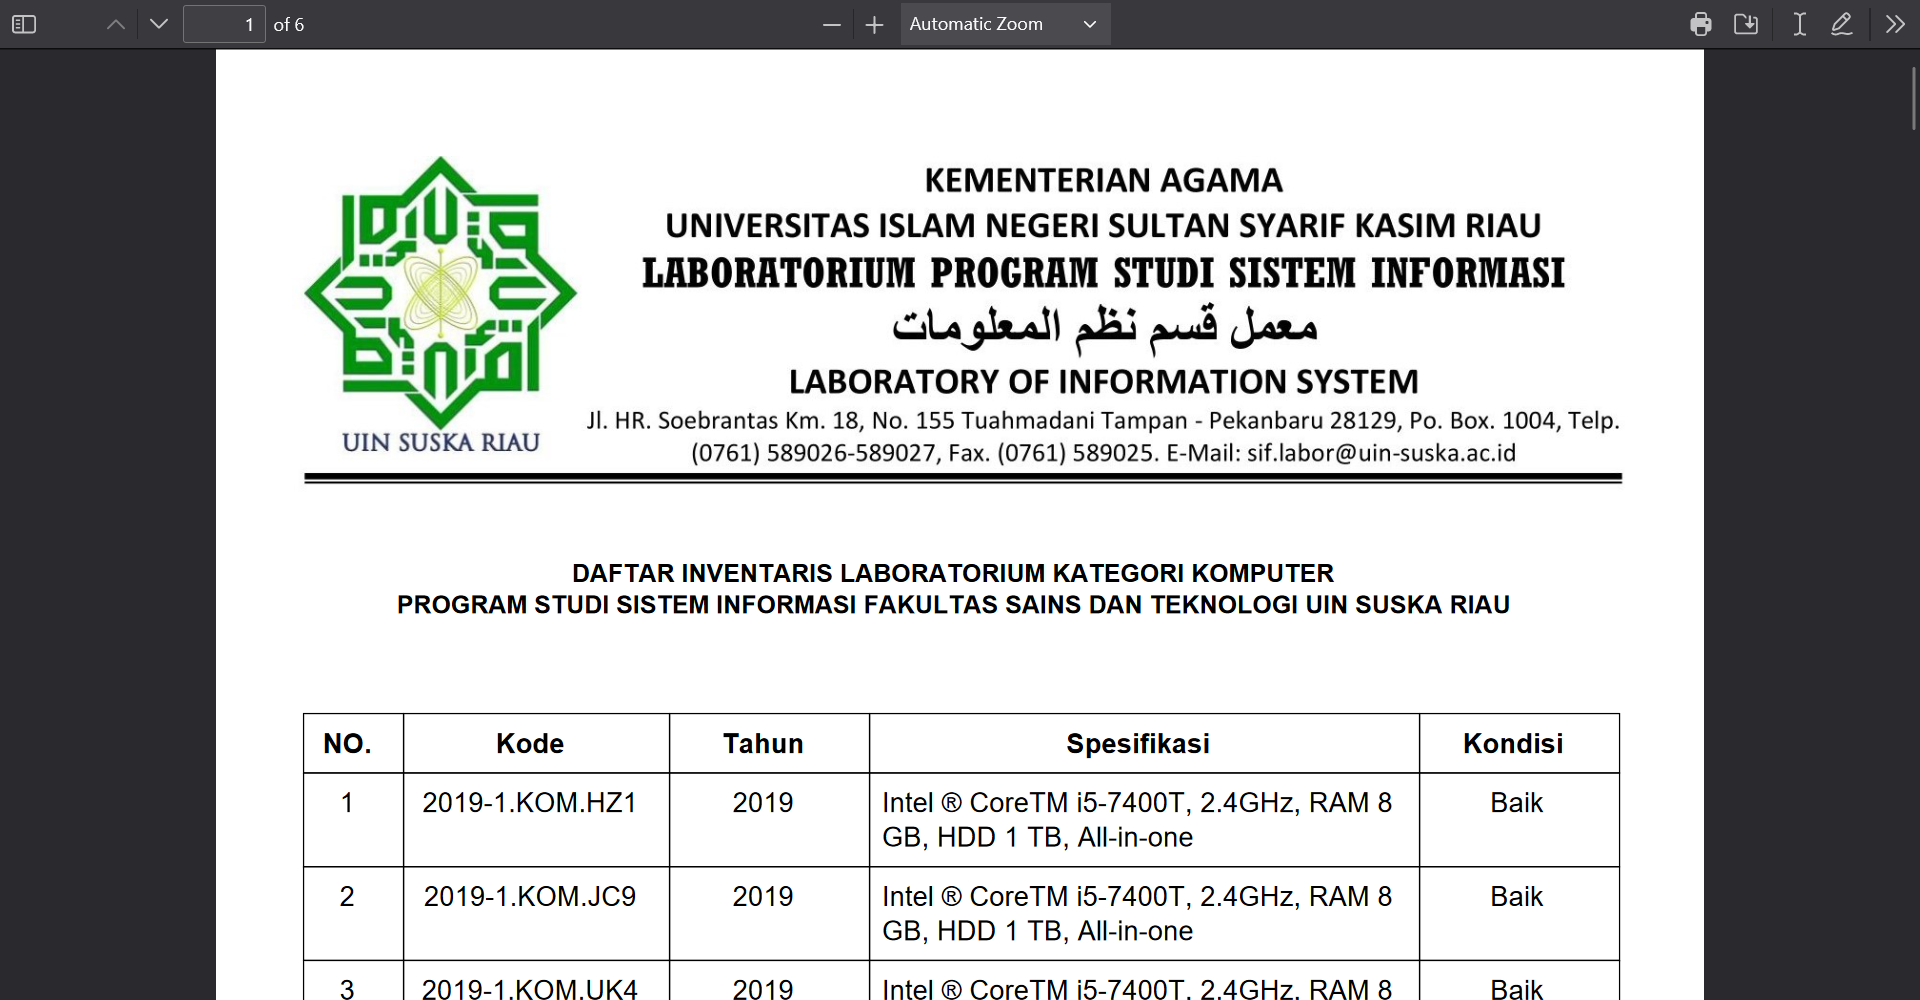
\includegraphics[width=0.82\linewidth]{konten//gambar/barang cetak kategori pdf.png}
          \caption{Halaman Cetak Kategori}
          \label{fig:enter-label}
        \end{figure}

  \item Halaman Posisi Barang \\ Halaman posisi barang merupakan tampilan untuk melihat dan mengelola data barang berdasarkan posisi barang, terdapat tombol berwarna biru toska yang dibedakan menjadi beberapa tombol yang bertujuan untuk mencetak dokumen laporan berdasarkan data ruangan yang sedang ditampilkan, pendanaan, kategori, tahun, dan QR seperti pada Gambar 2.20. sampai Gambar 2.22.

        \begin{figure}
          \centering
          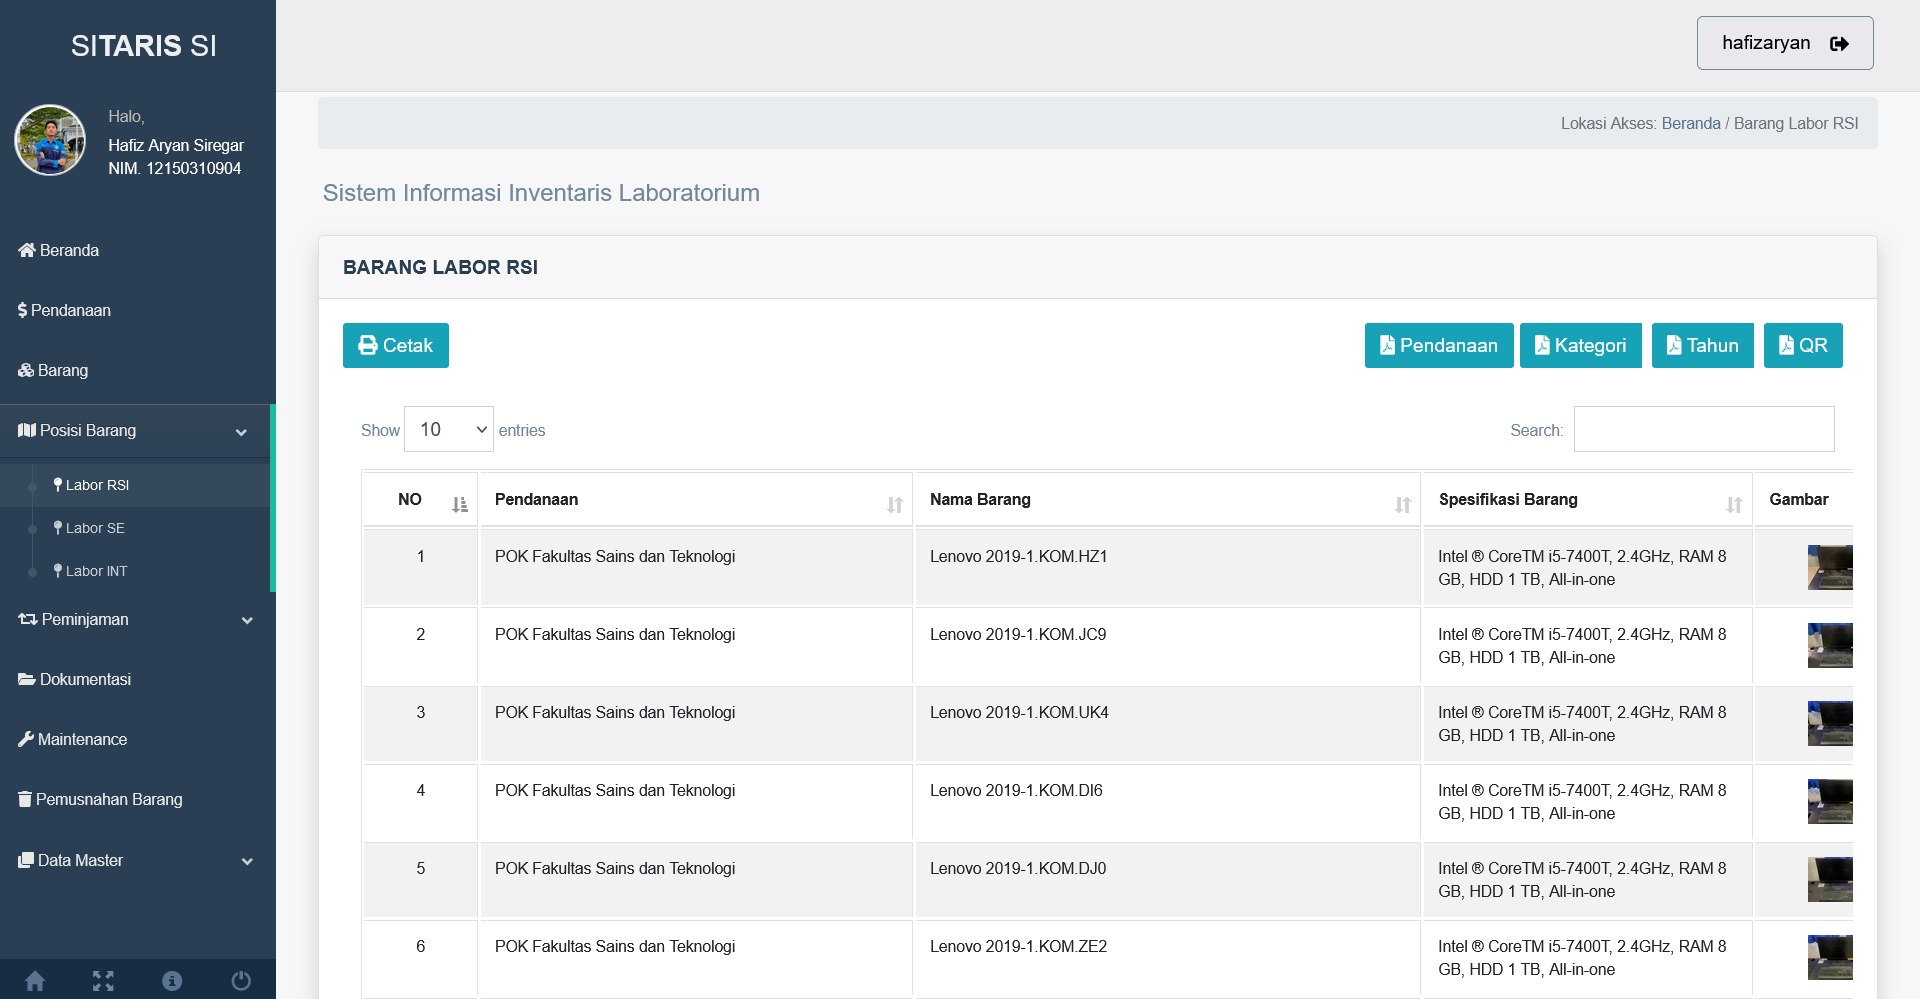
\includegraphics[width=0.82\linewidth]{konten//gambar/rsi.png}
          \caption{Halaman Posisi Barang Labor RSI}
          \label{fig:enter-label}
        \end{figure}

        \begin{figure}
          \centering
          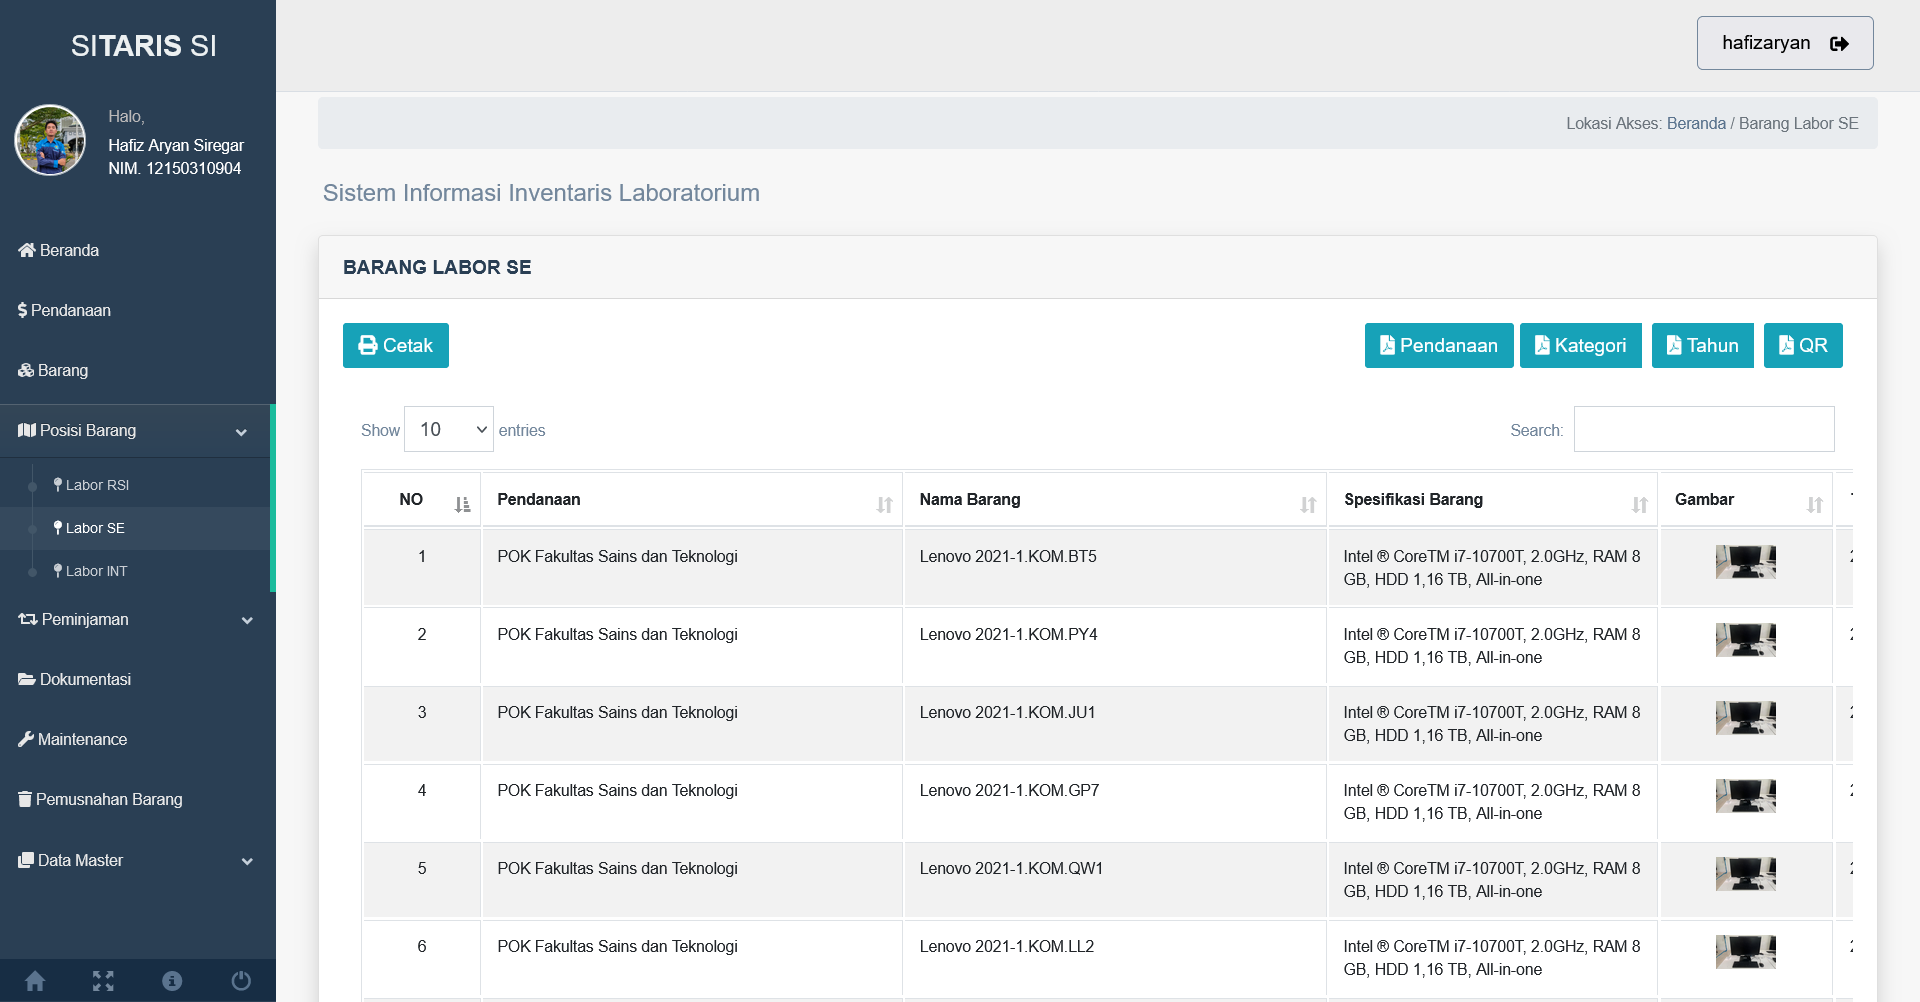
\includegraphics[width=0.82\linewidth]{konten//gambar/se.png}
          \caption{Halaman Posisi Barang Labor SE}
          \label{fig:enter-label}
        \end{figure}

        \begin{figure}
          \centering
          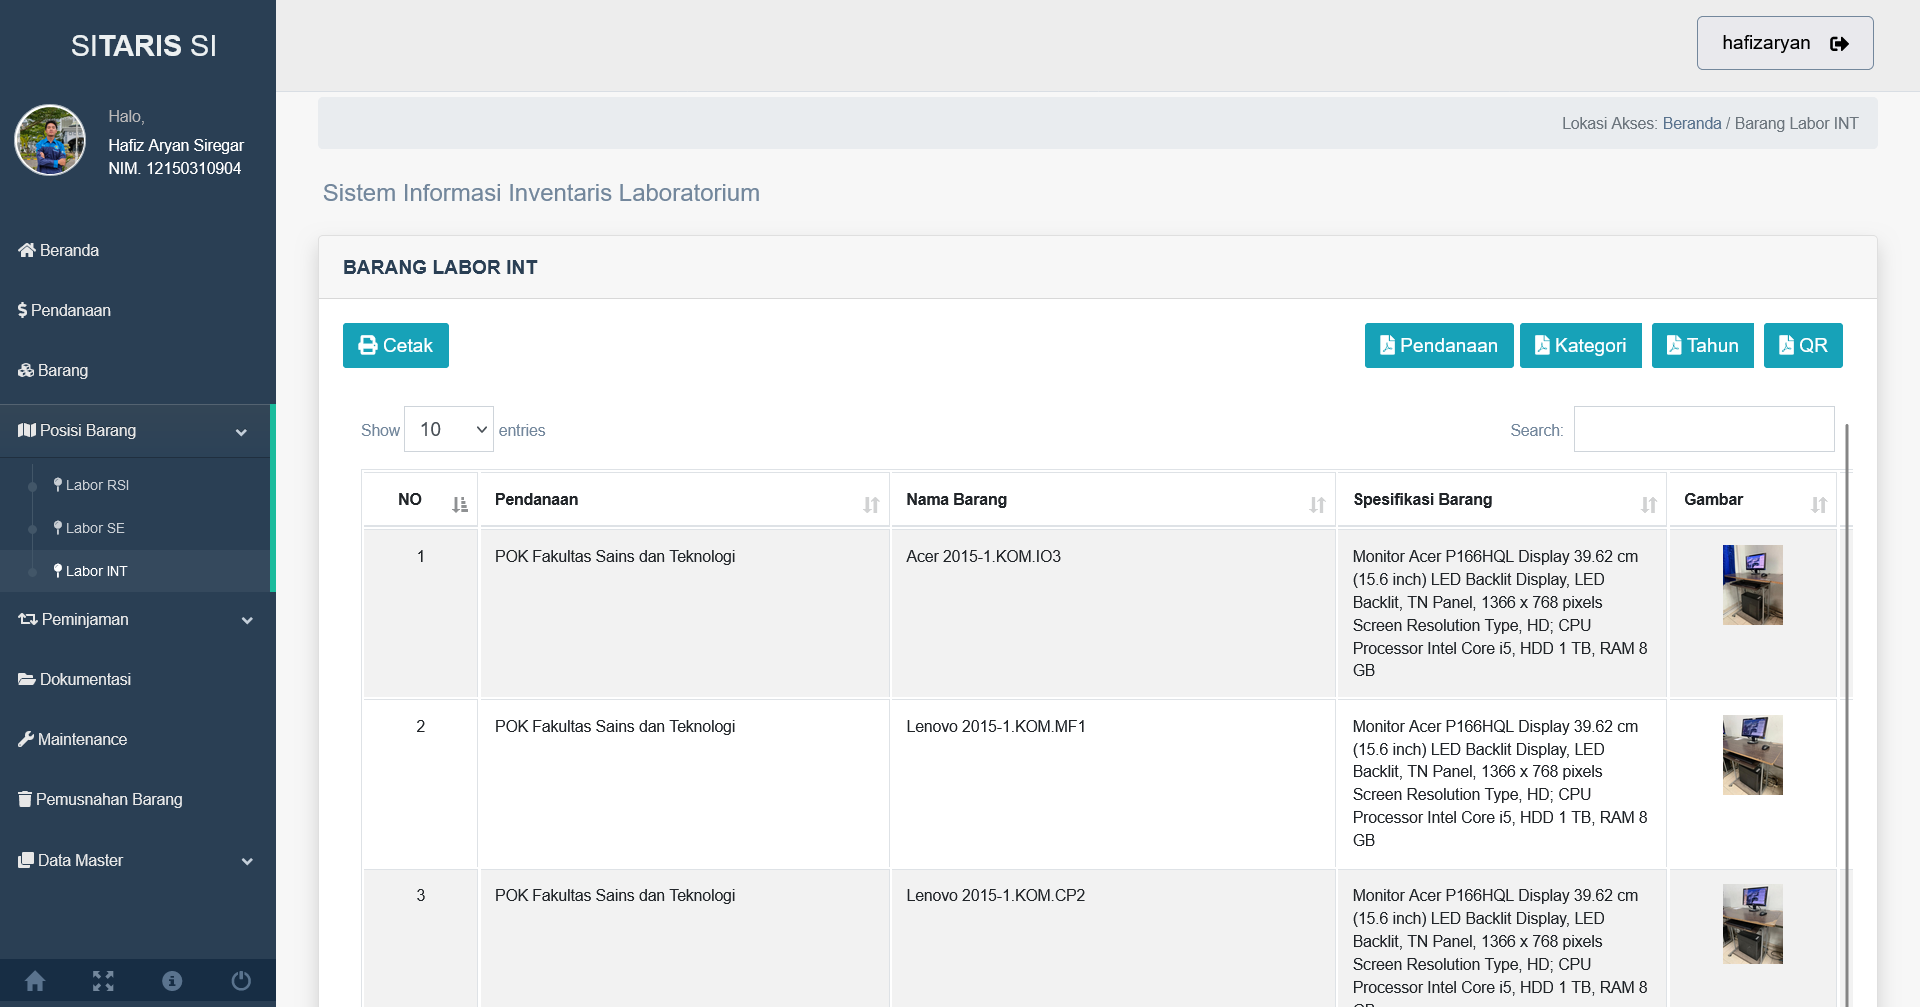
\includegraphics[width=0.82\linewidth]{konten//gambar/int.png}
          \caption{Halaman Posisi Barang Labor INT}
          \label{fig:enter-label}
        \end{figure}

  \item Halaman Peminjaman Barang \\ Halaman peminjaman barang merupakan tampilan untuk melihat dan mengelola data peminjaman barang, tombol \textit{trash} untuk menghapus data peminjaman barang. Lalu ada beberapa tahap yang dilakukan oleh peminjam untuk melakukan peminjaman barang seperti mengisi data peminjaman berdasarkan asal peminjam internal atau eksternal seperti pada Gambar 2.24. sampai Gambar 2.30.

        \begin{figure}
          \centering
          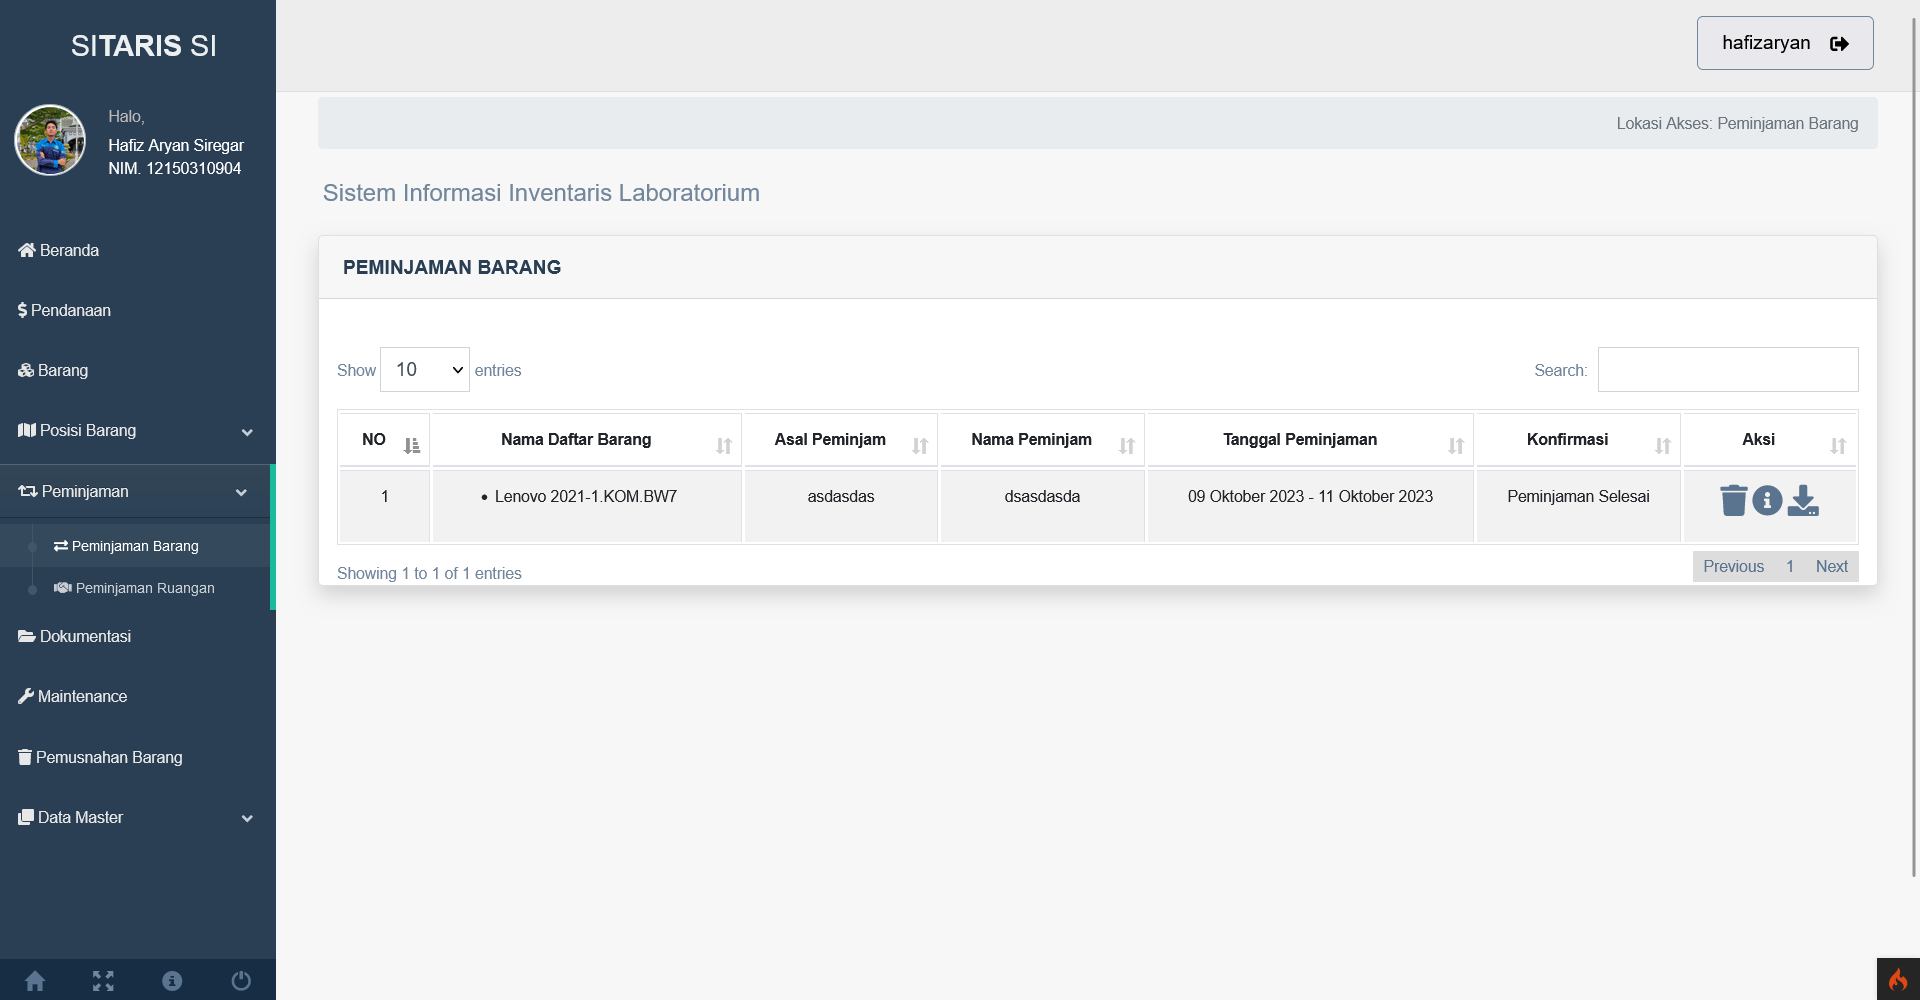
\includegraphics[width=0.82\linewidth]{konten//gambar/peminjaman barang index hasil.png}
          \caption{Halaman Peminjaman Barang \textit{Index}}
          \label{fig:enter-label}
        \end{figure}

        %   \begin{figure}
        %       \centering
        %       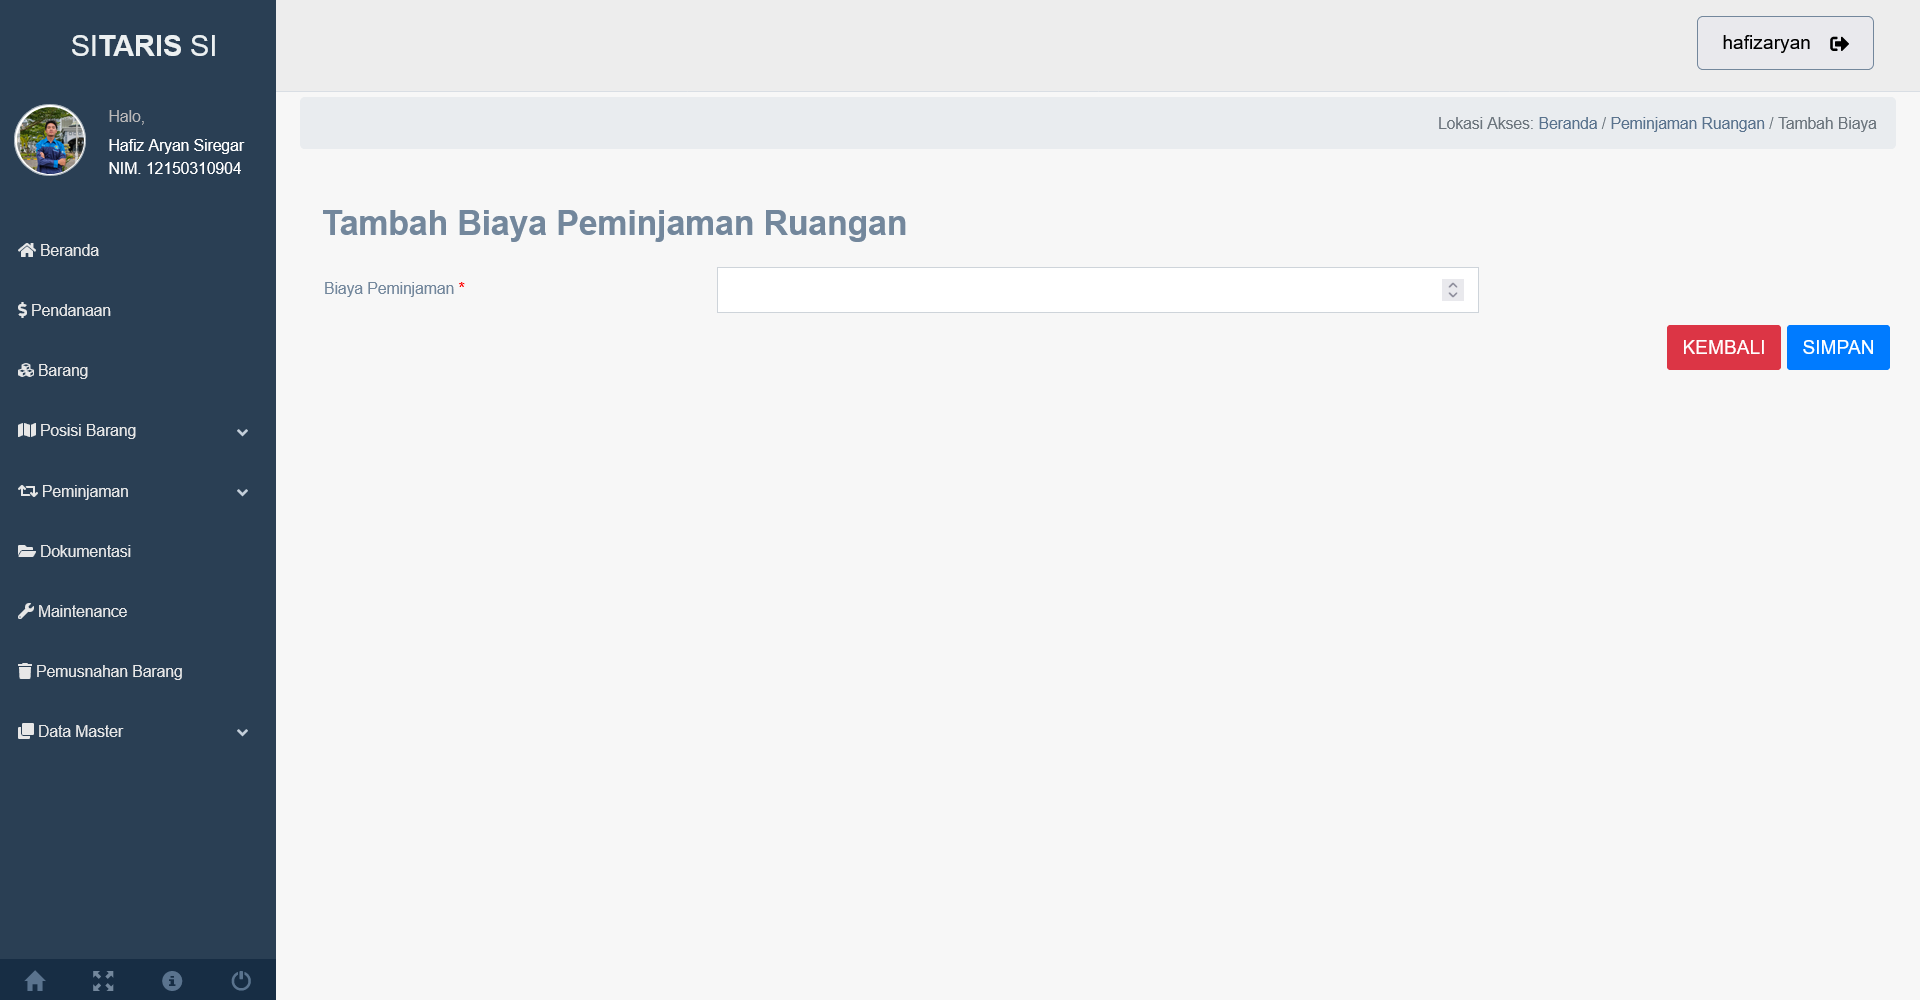
\includegraphics[width=0.82\linewidth]{konten//gambar/tambah biaya peminjaman ruangan.png}
        %       \caption{Halaman Tambah Biaya Peminjaman Ruangan}
        %       \label{fig:enter-label}
        %   \end{figure}

        \begin{figure}
          \centering
          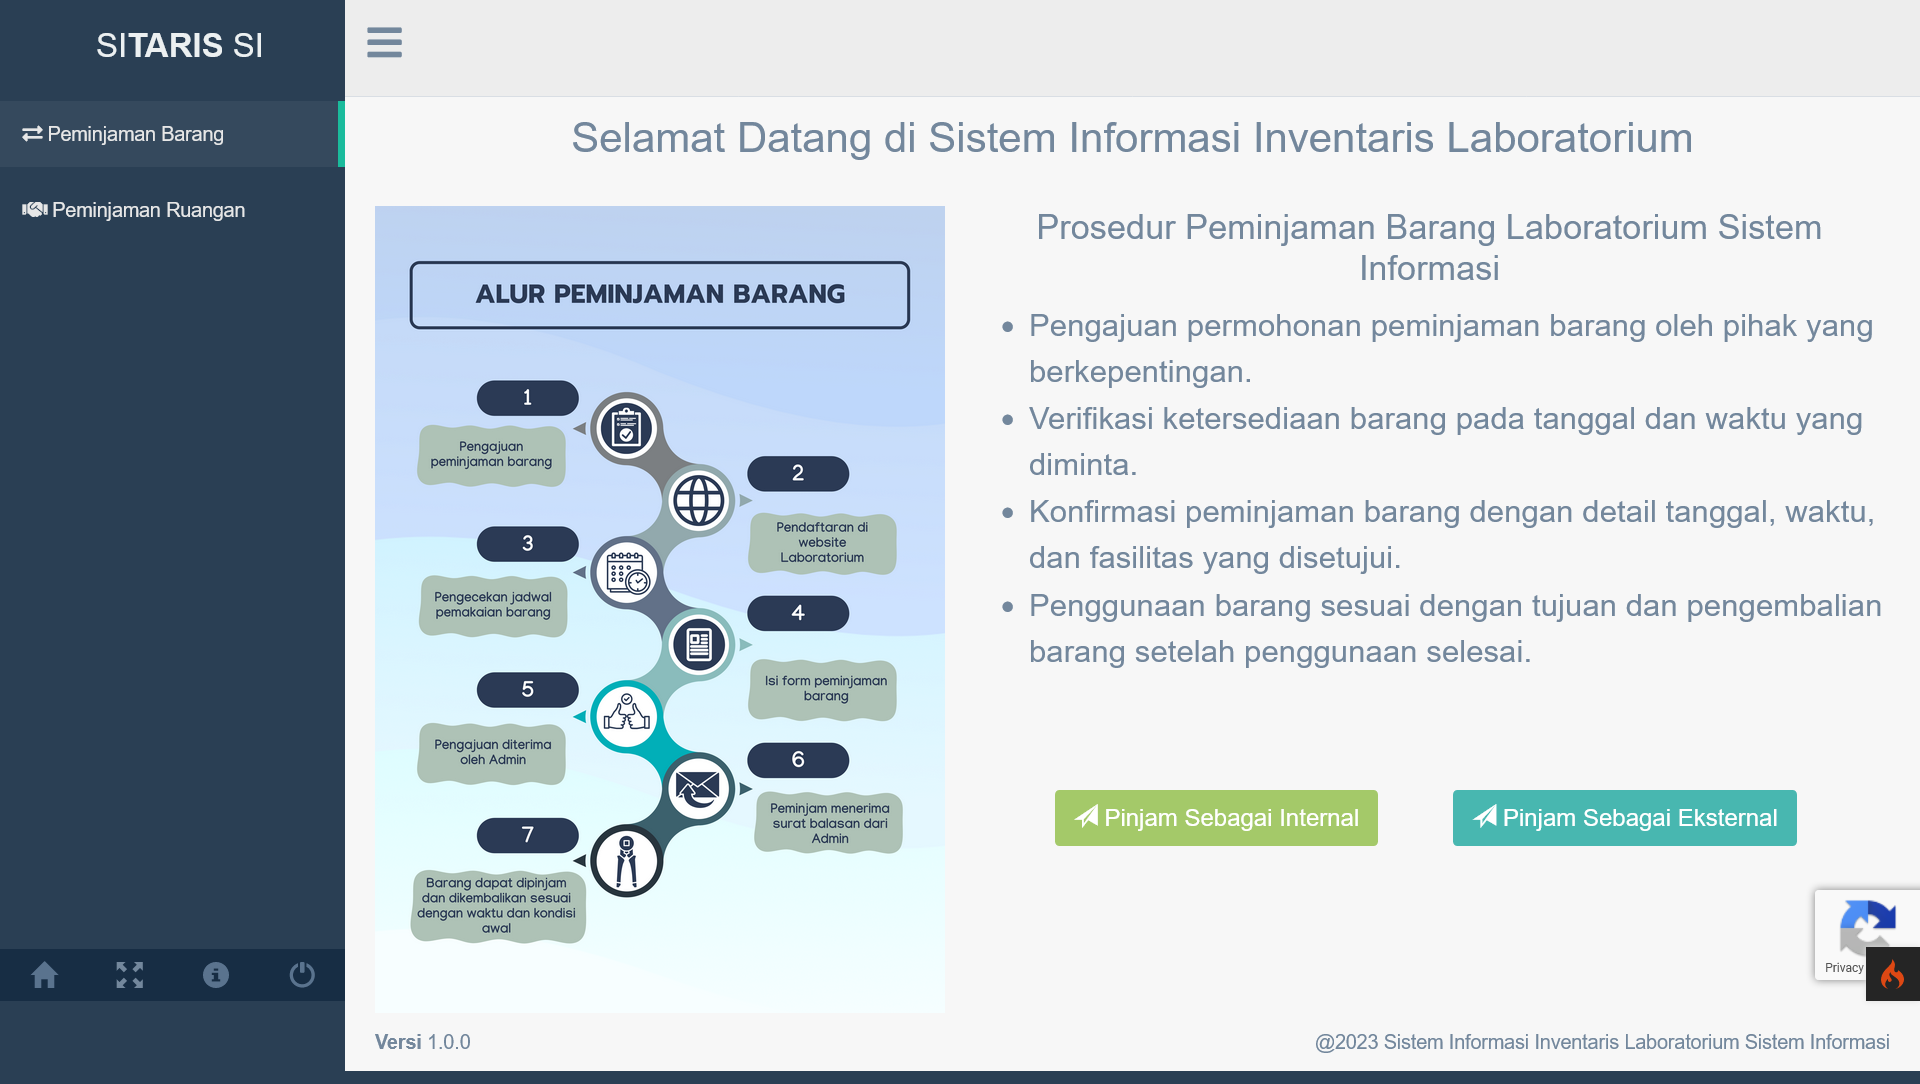
\includegraphics[width=0.82\linewidth]{konten//gambar/peminjaman barang pinjam hasil.png}
          \caption{Halaman Peminjaman Barang Bagi Peminjam}
          \label{fig:enter-label}
        \end{figure}

        \begin{figure}
          \centering
          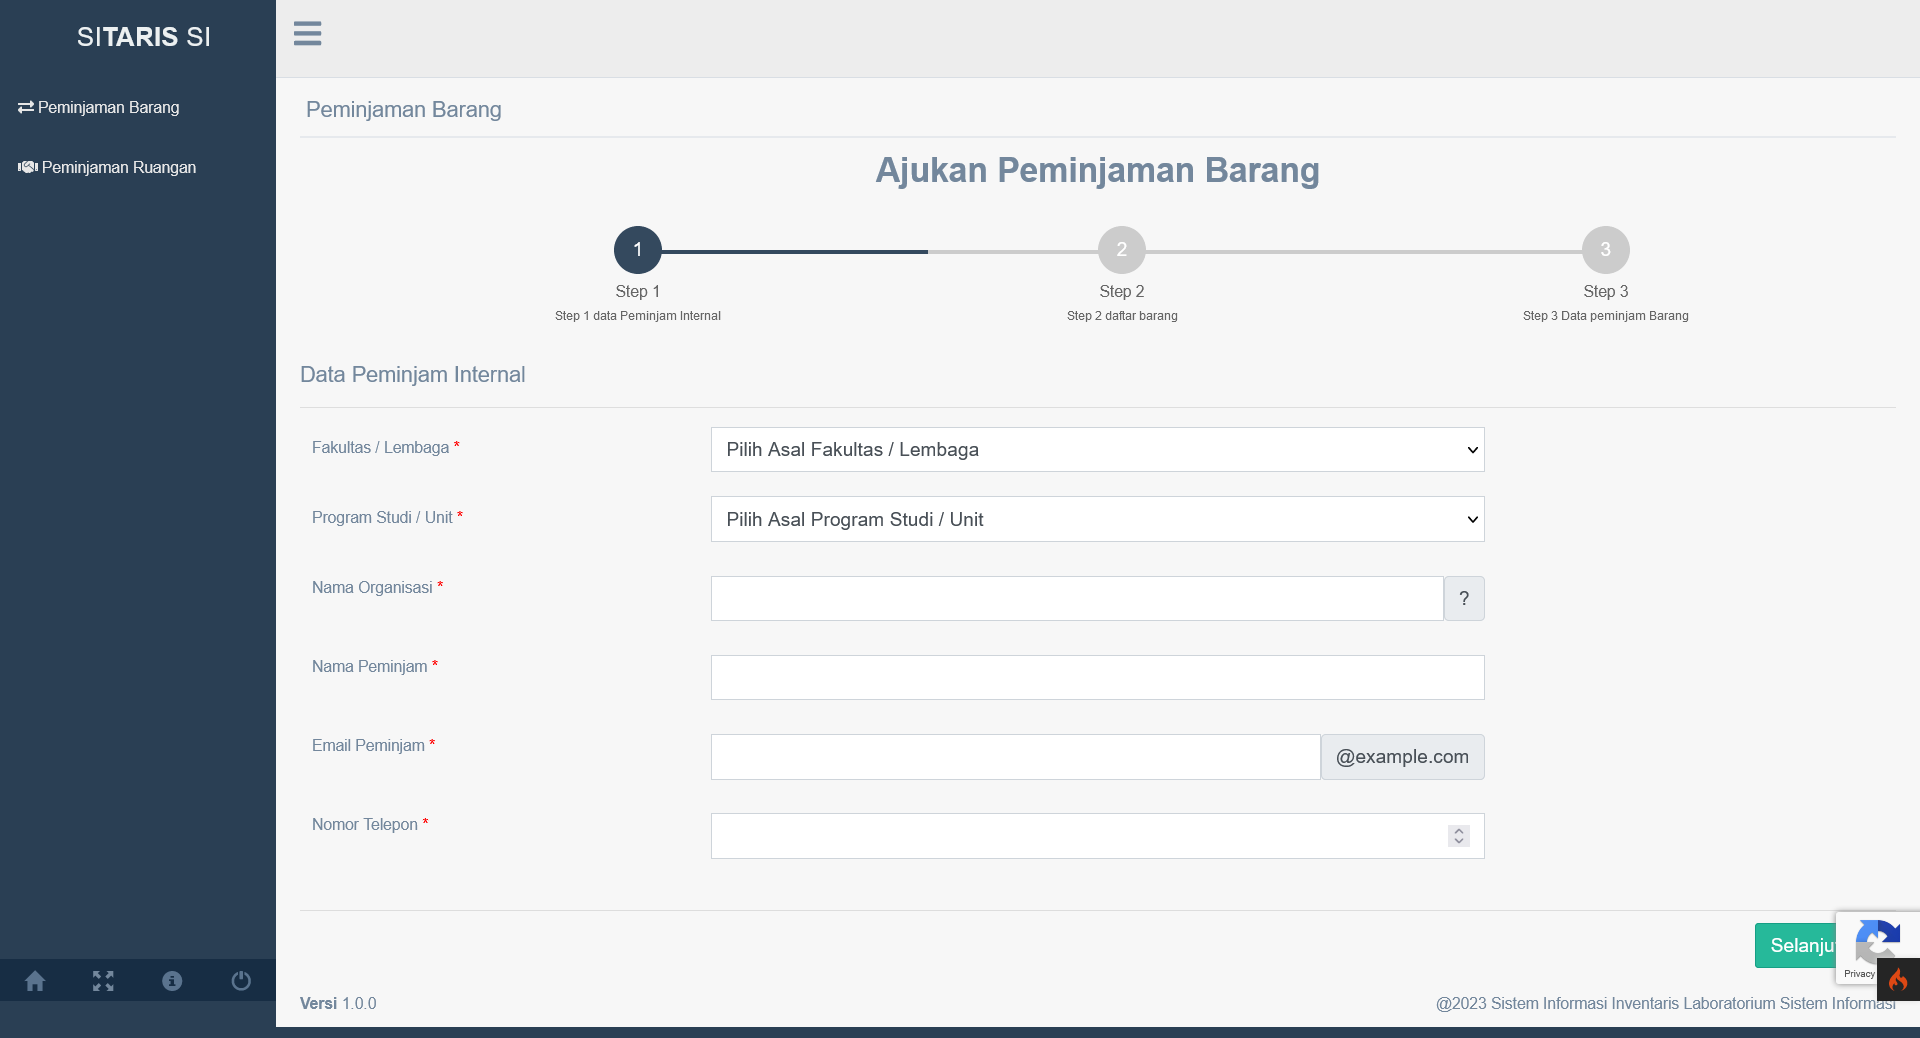
\includegraphics[width=0.82\linewidth]{konten//gambar/peminjaman barang tambah internal 1 hasil.png}
          \caption{Halaman Peminjaman Barang Bagi Peminjam Internal Tahap 1}
          \label{fig:enter-label}
        \end{figure}

        \begin{figure}
          \centering
          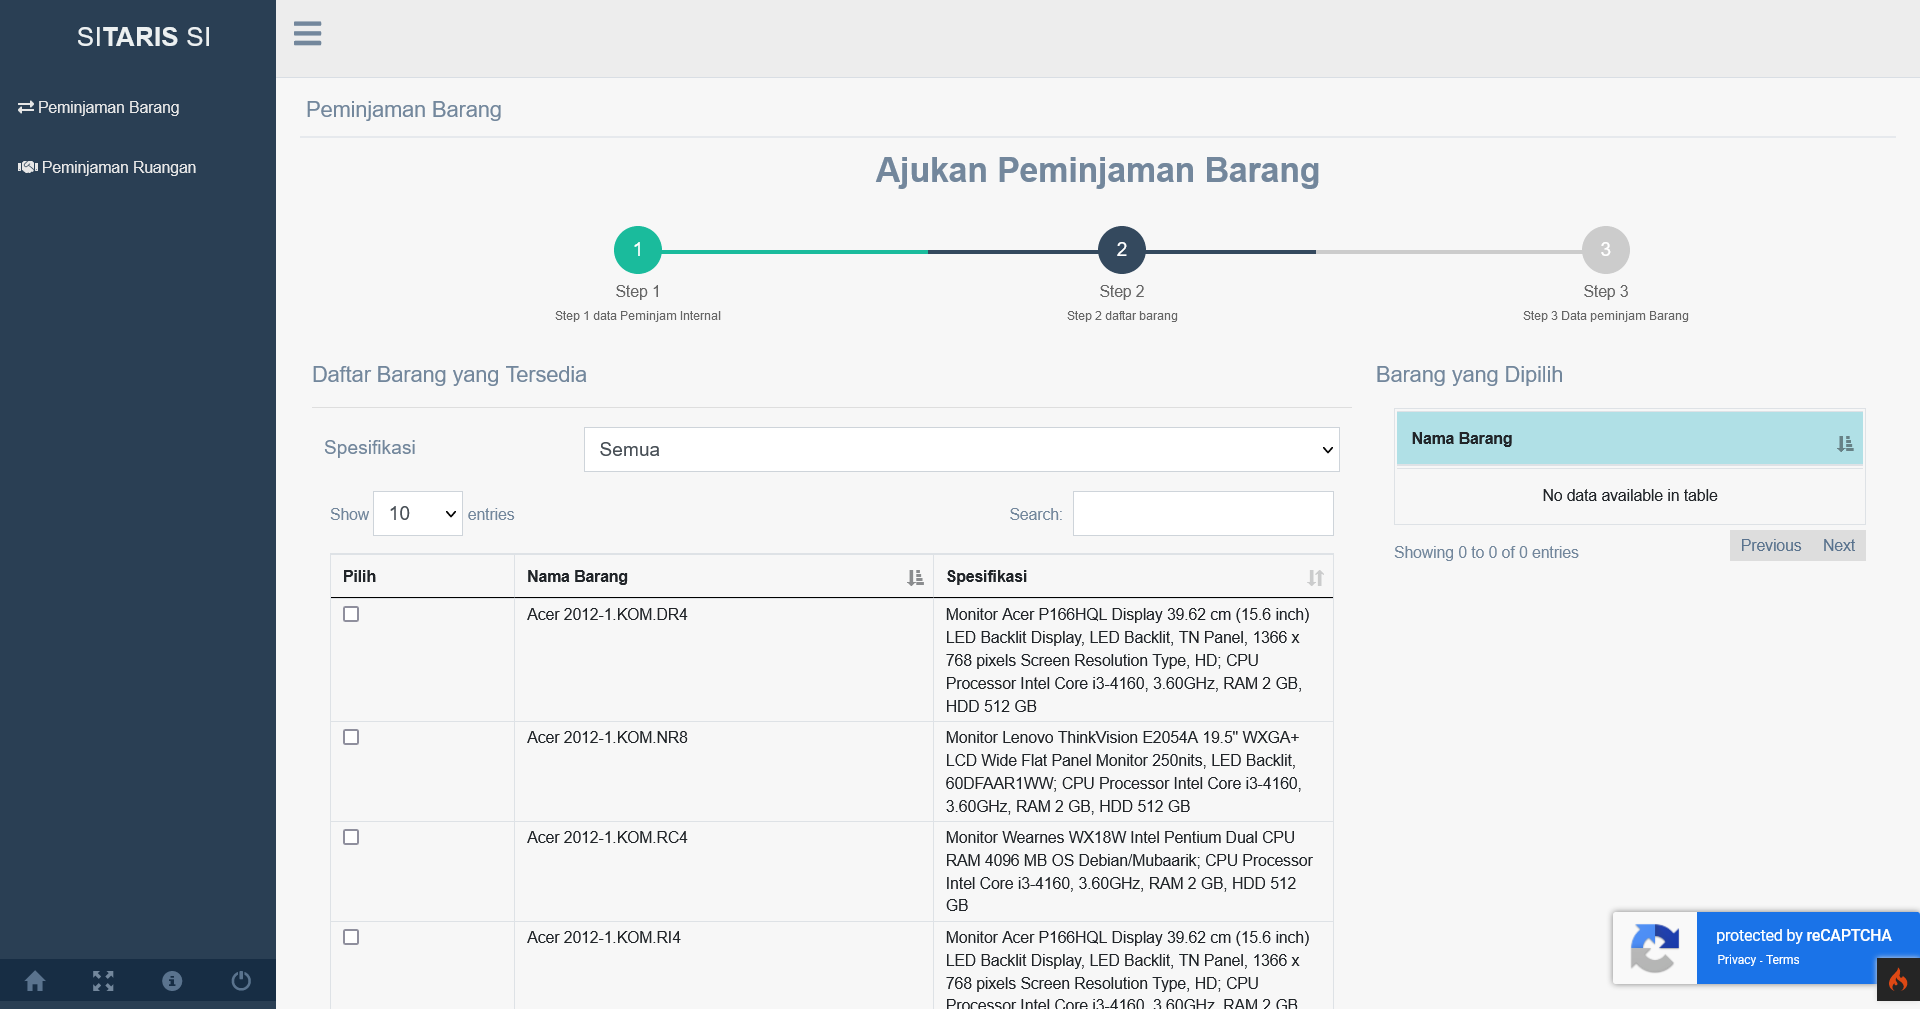
\includegraphics[width=0.82\linewidth]{konten//gambar/peminjaman barang tambah internal 2 hasil.png}
          \caption{Halaman Peminjaman Barang Bagi Peminjam Internal Tahap 2}
          \label{fig:enter-label}
        \end{figure}

        \begin{figure}
          \centering
          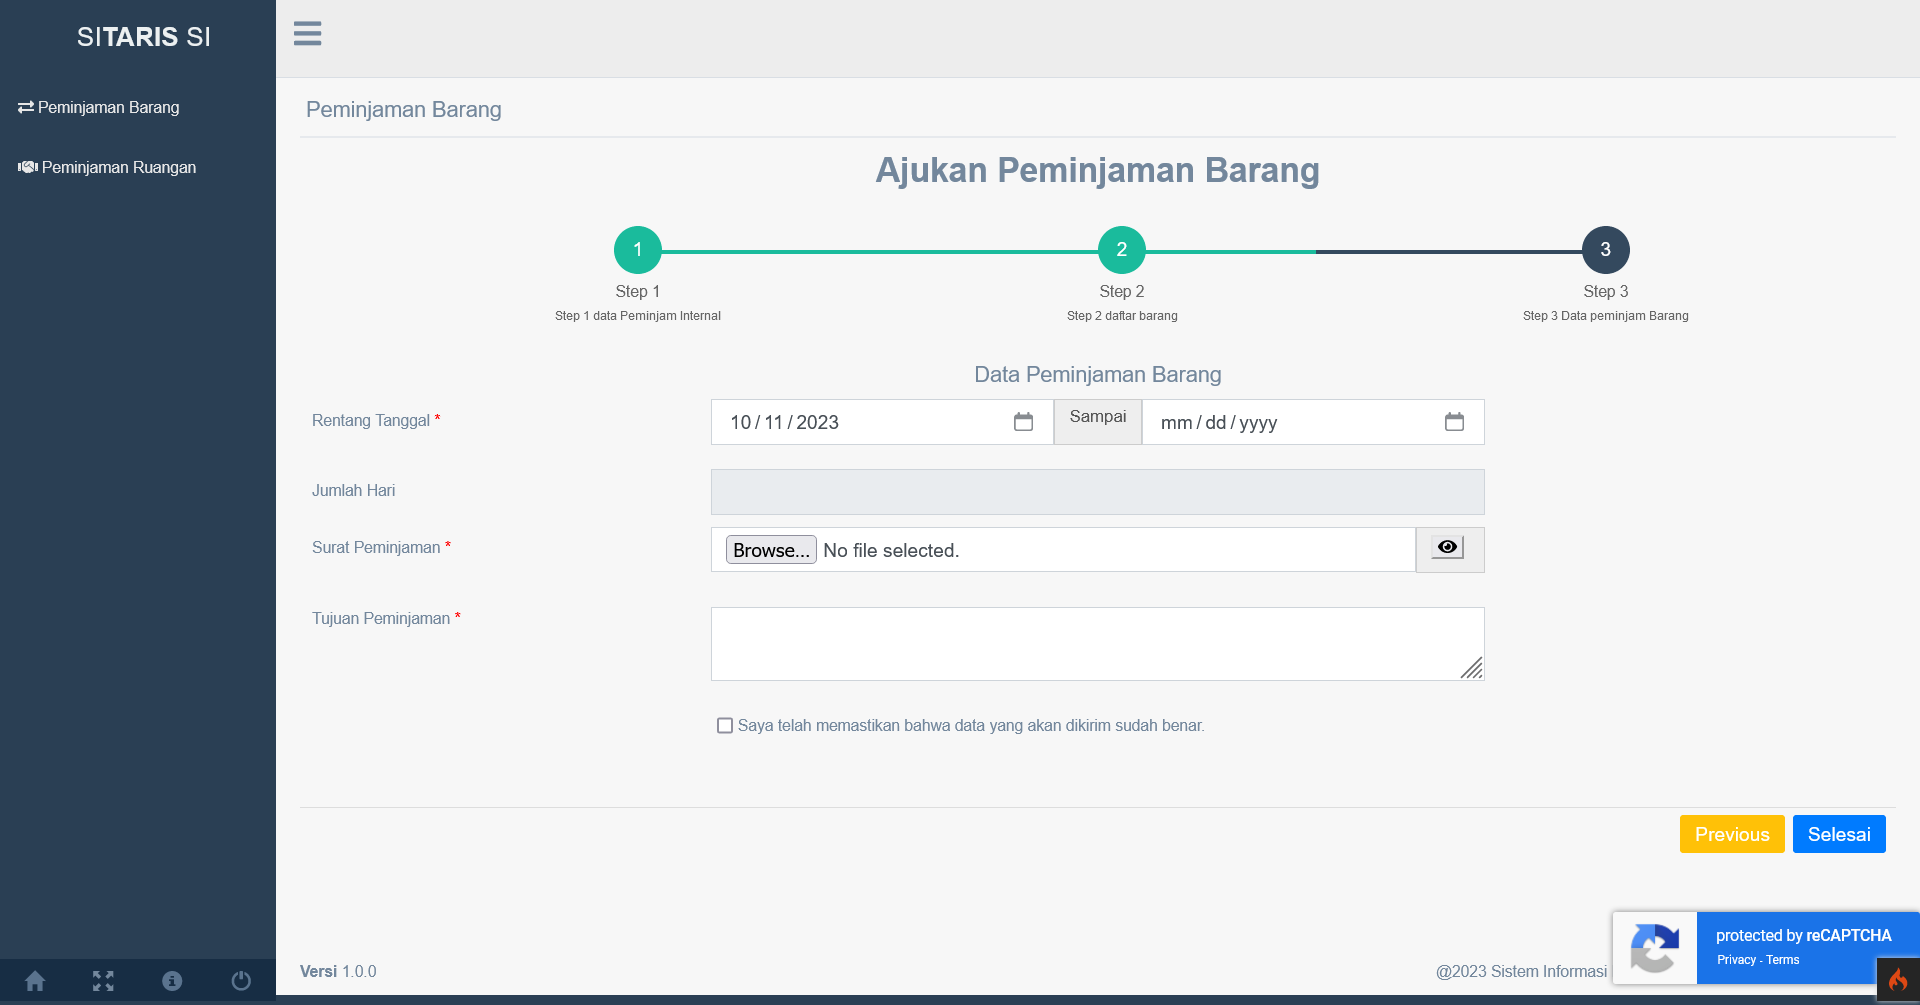
\includegraphics[width=0.82\linewidth]{konten//gambar/peminjaman barang tambah internal 3 hasil.png}
          \caption{Halaman Peminjaman Barang Bagi Peminjam Internal Tahap 3}
          \label{fig:enter-label}
        \end{figure}

        \begin{figure}
          \centering
          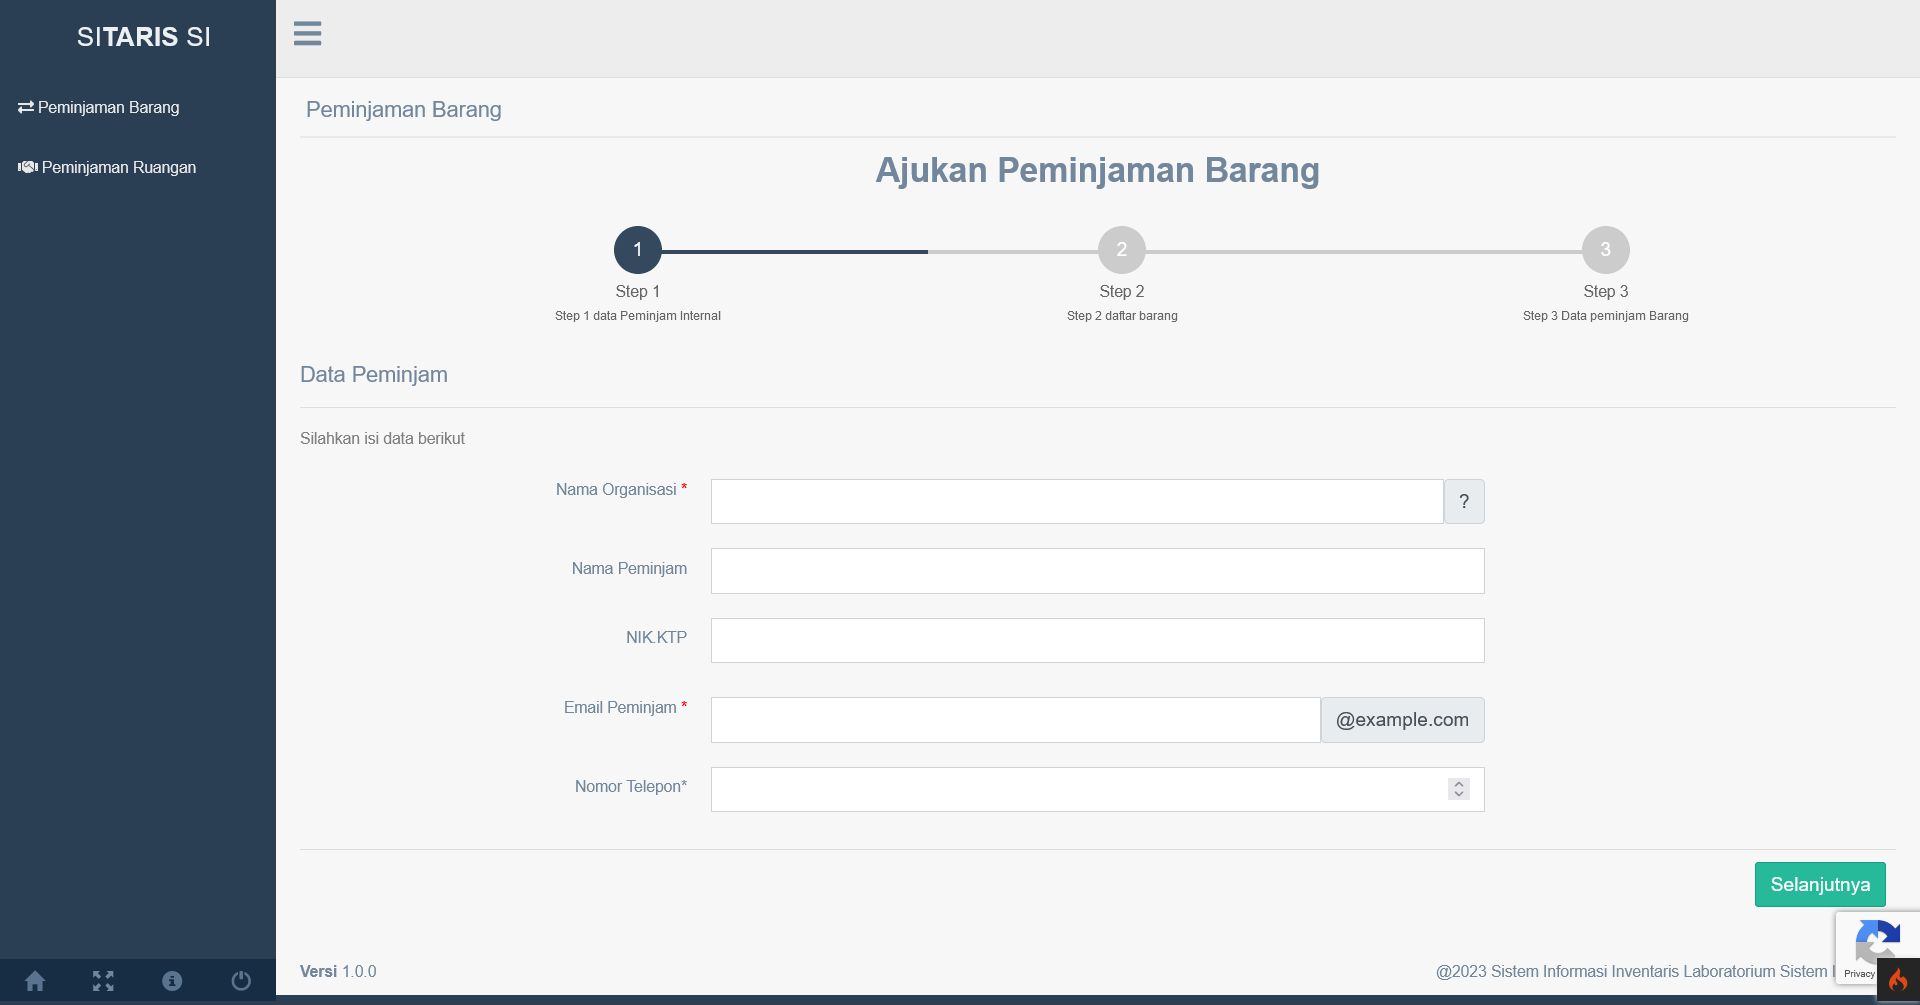
\includegraphics[width=0.82\linewidth]{konten//gambar/peminjaman barang tambah eksternal 1 hasil.png}
          \caption{Halaman Peminjaman Barang Bagi Peminjam Eksternal Tahap 1}
          \label{fig:enter-label}
        \end{figure}

        \begin{figure}
          \centering
          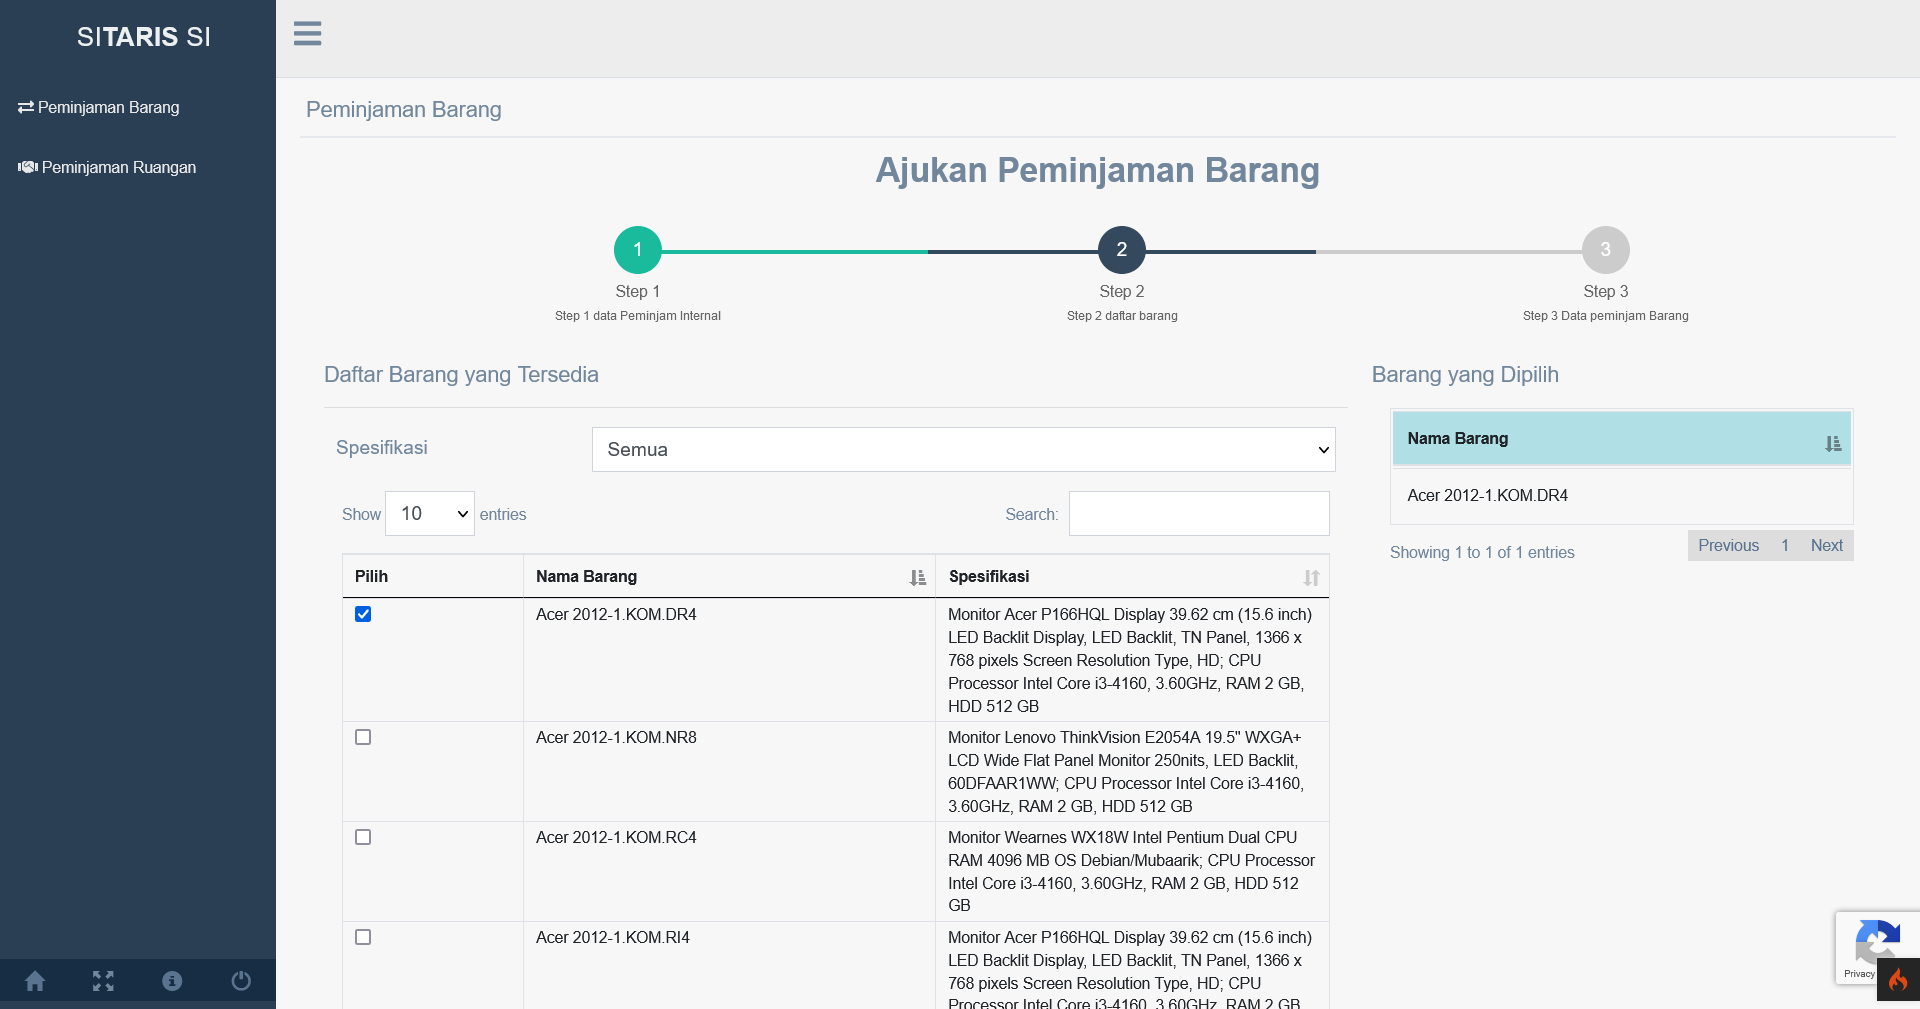
\includegraphics[width=0.82\linewidth]{konten//gambar/peminjaman barang tambah eksternal 2 hasil.png}
          \caption{Halaman Peminjaman Barang Bagi Peminjam Eksternal Tahap 2}
          \label{fig:enter-label}
        \end{figure}

        \begin{figure}
          \centering
          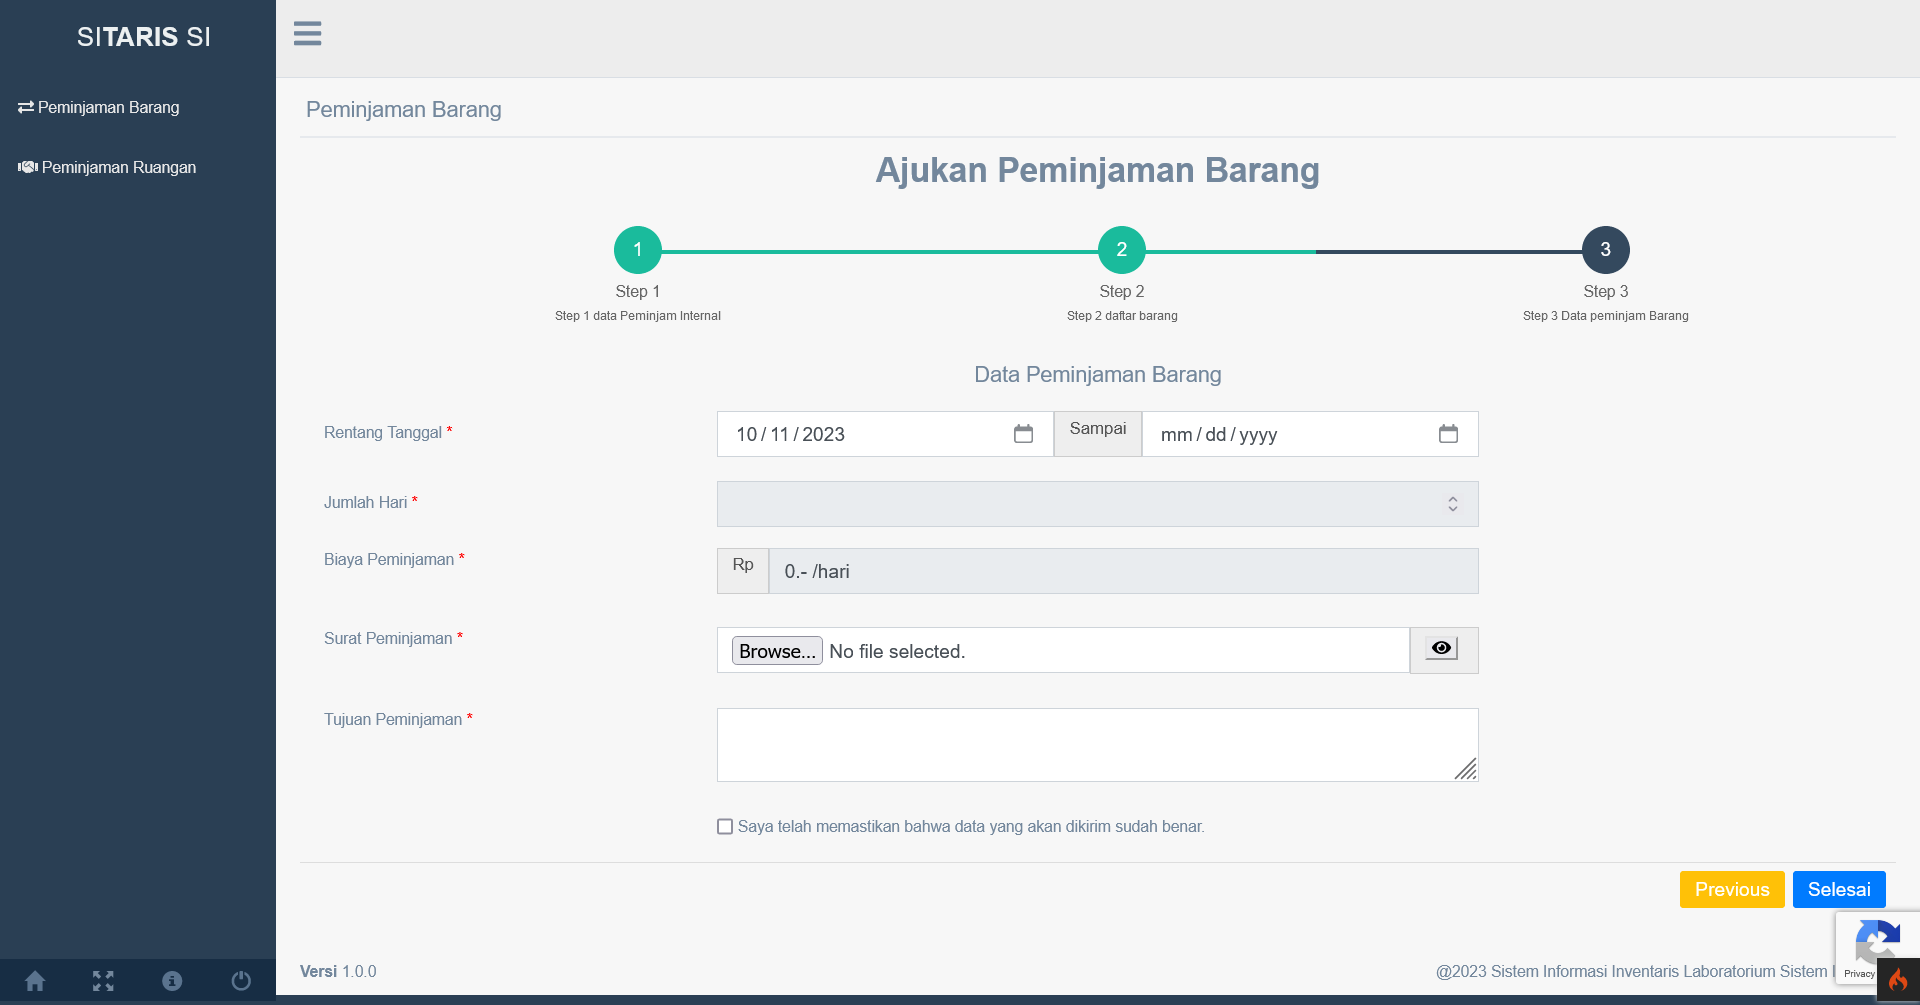
\includegraphics[width=0.82\linewidth]{konten//gambar/peminjaman barang tambah eksternal 3 hasil.png}
          \caption{Halaman Peminjaman Barang Bagi Peminjam Eksternal Tahap 3}
          \label{fig:enter-label}
        \end{figure}

  \item Halaman Peminjaman Ruangan \\ Halaman peminjaman ruangan merupakan tampilan untuk melihat dan mengelola data peminjaman ruangan, tombol \textit{trash} untuk menghapus data peminjaman ruangan. Lalu ada beberapa tahap yang dilakukan oleh peminjam untuk melakukan peminjaman ruangan seperti mengisi data peminjaman berdasarkan asal peminjam internal atau eksternal seperti pada Gambar 2.31. sampai Gambar 2.35.

        \begin{figure}
          \centering
          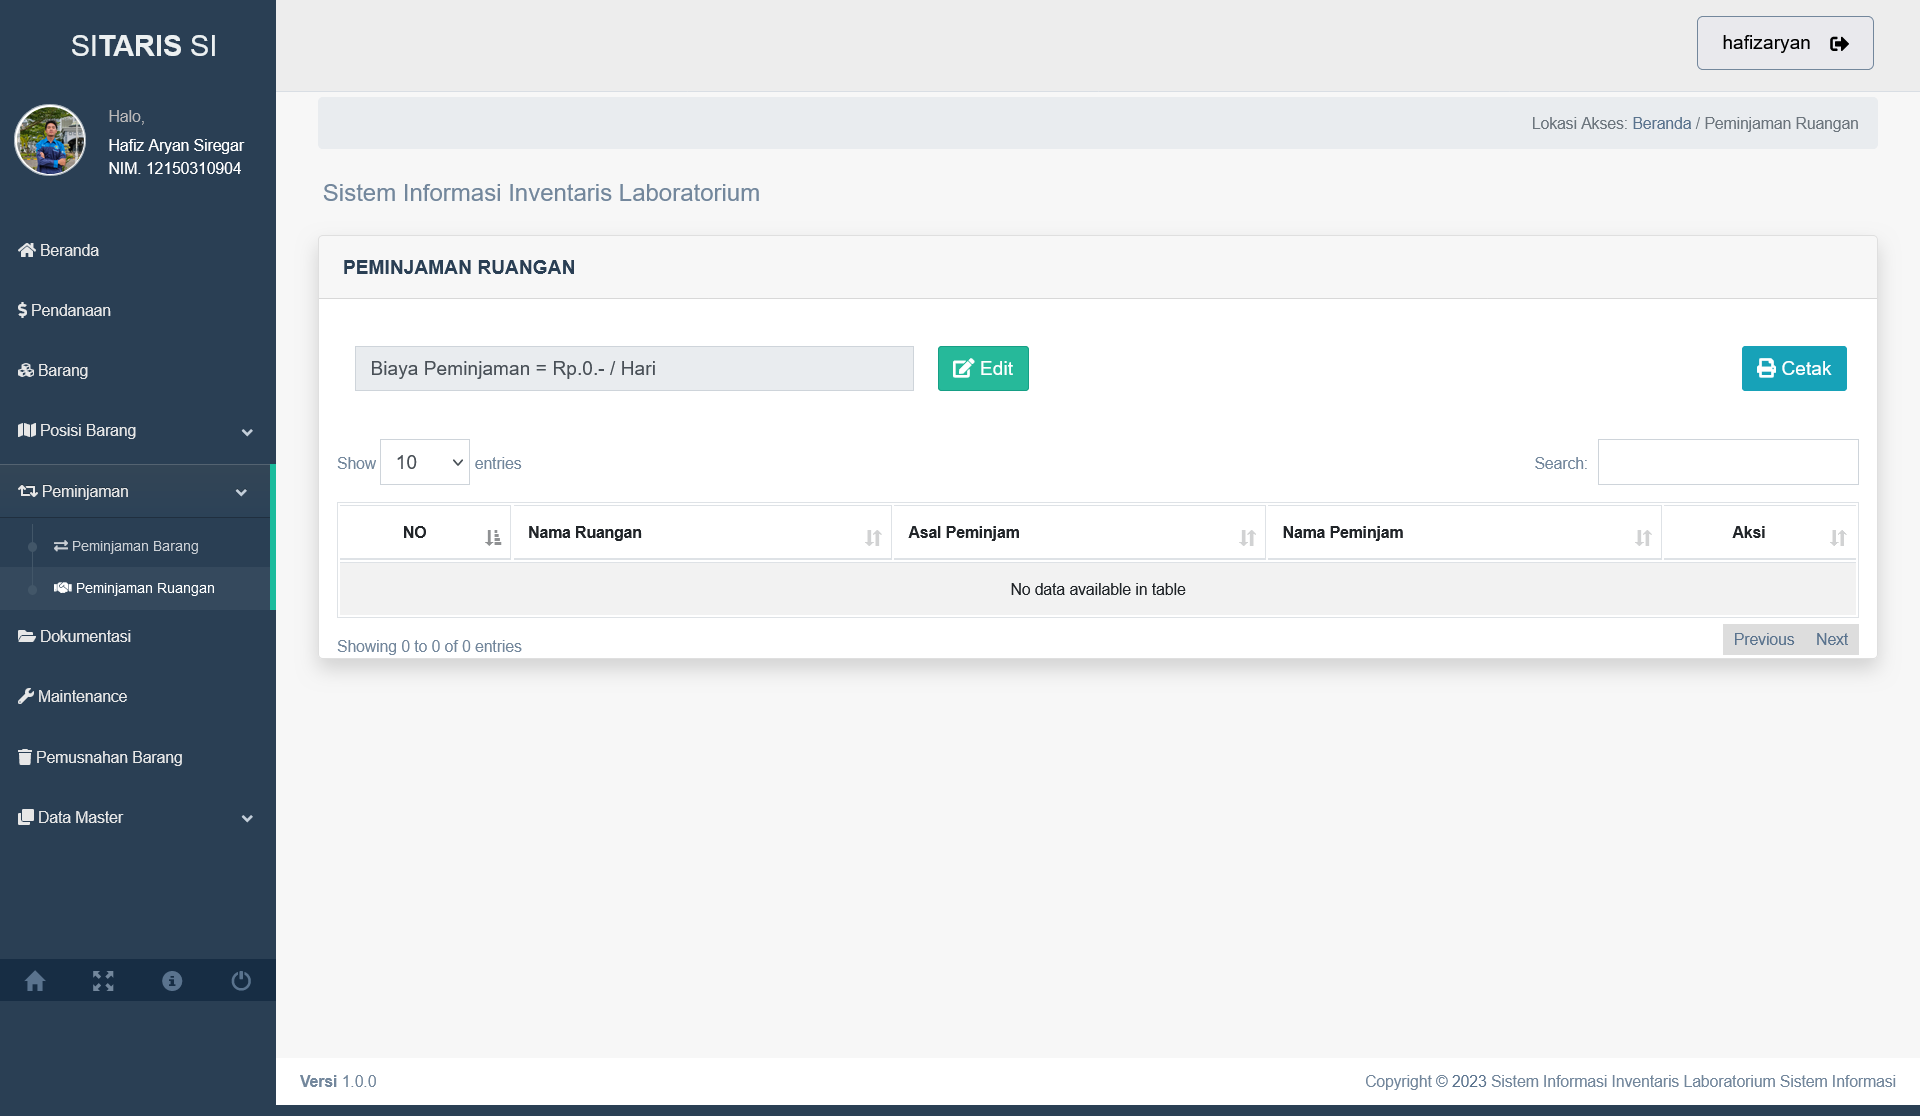
\includegraphics[width=0.82\linewidth]{konten//gambar/peminjaman ruangan index.png}
          \caption{Halaman Peminjaman Ruangan \textit{Index}}
          \label{fig:enter-label}
        \end{figure}

        \begin{figure}
          \centering
          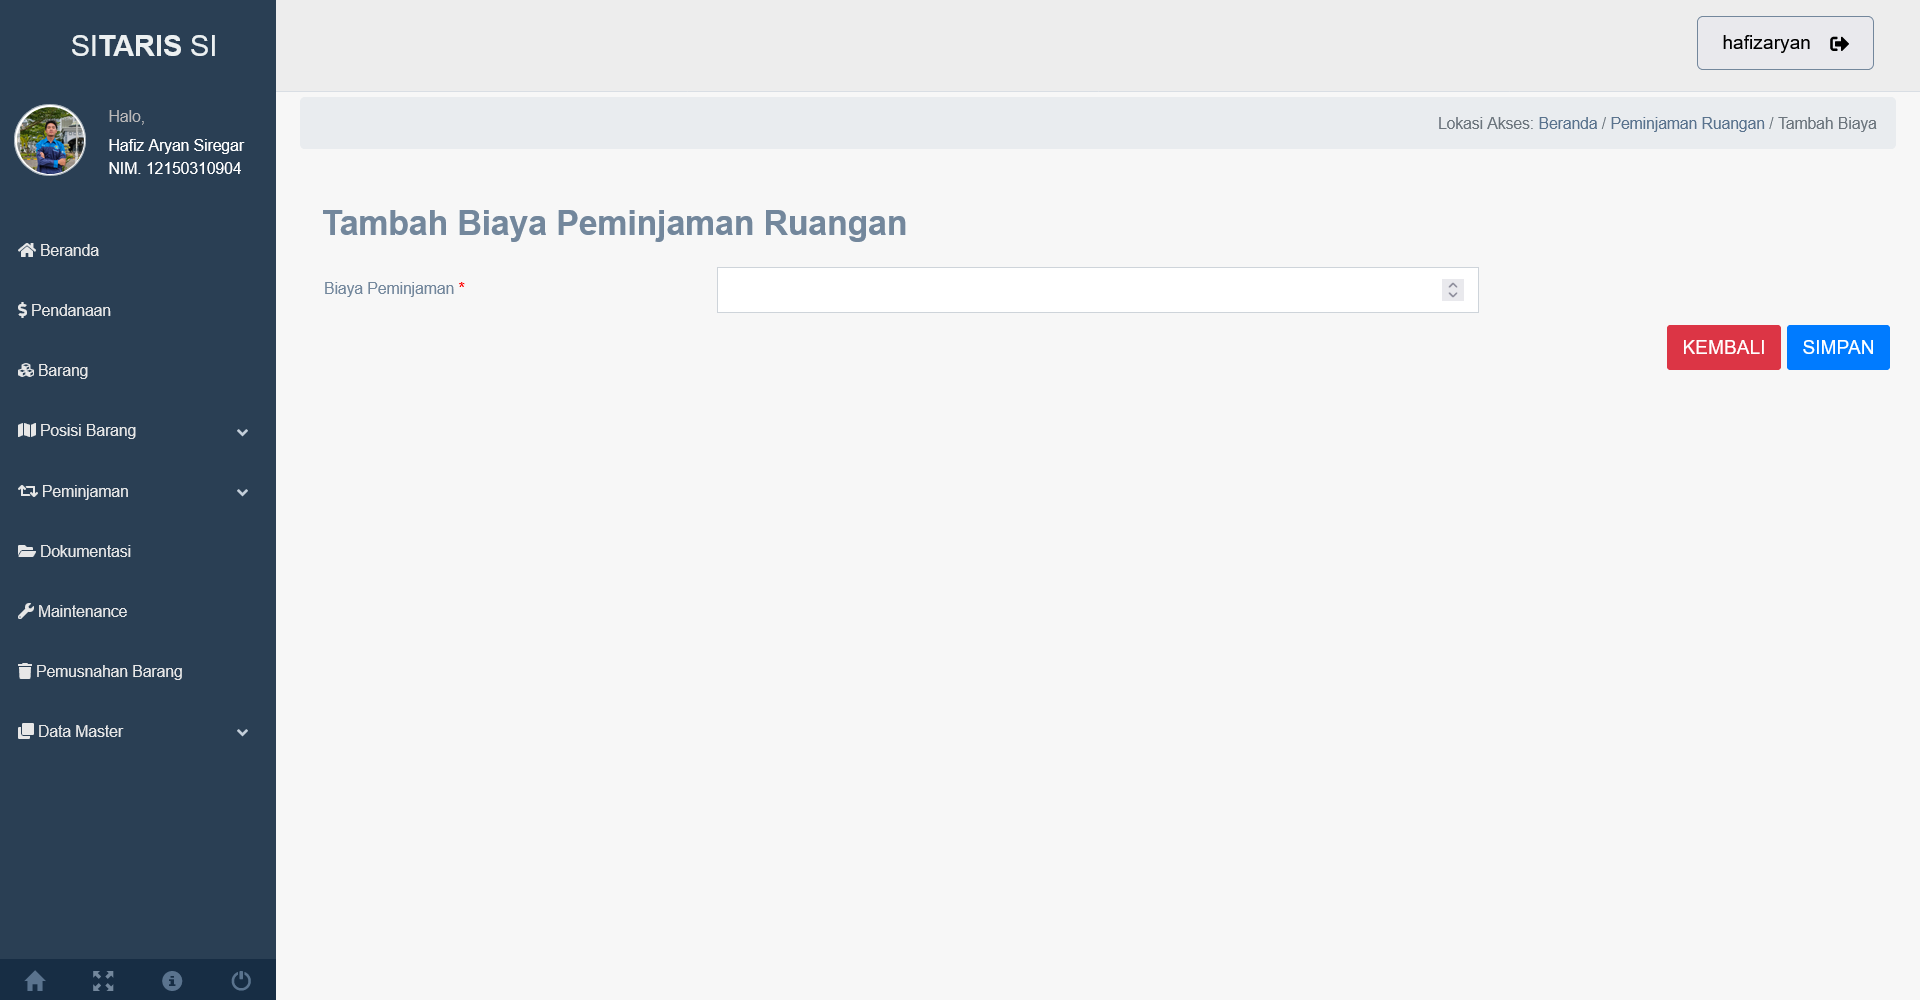
\includegraphics[width=0.82\linewidth]{konten//gambar/tambah biaya peminjaman ruangan.png}
          \caption{Halaman Tambah Biaya Peminjaman Ruangan}
          \label{fig:enter-label}
        \end{figure}

        \begin{figure}
          \centering
          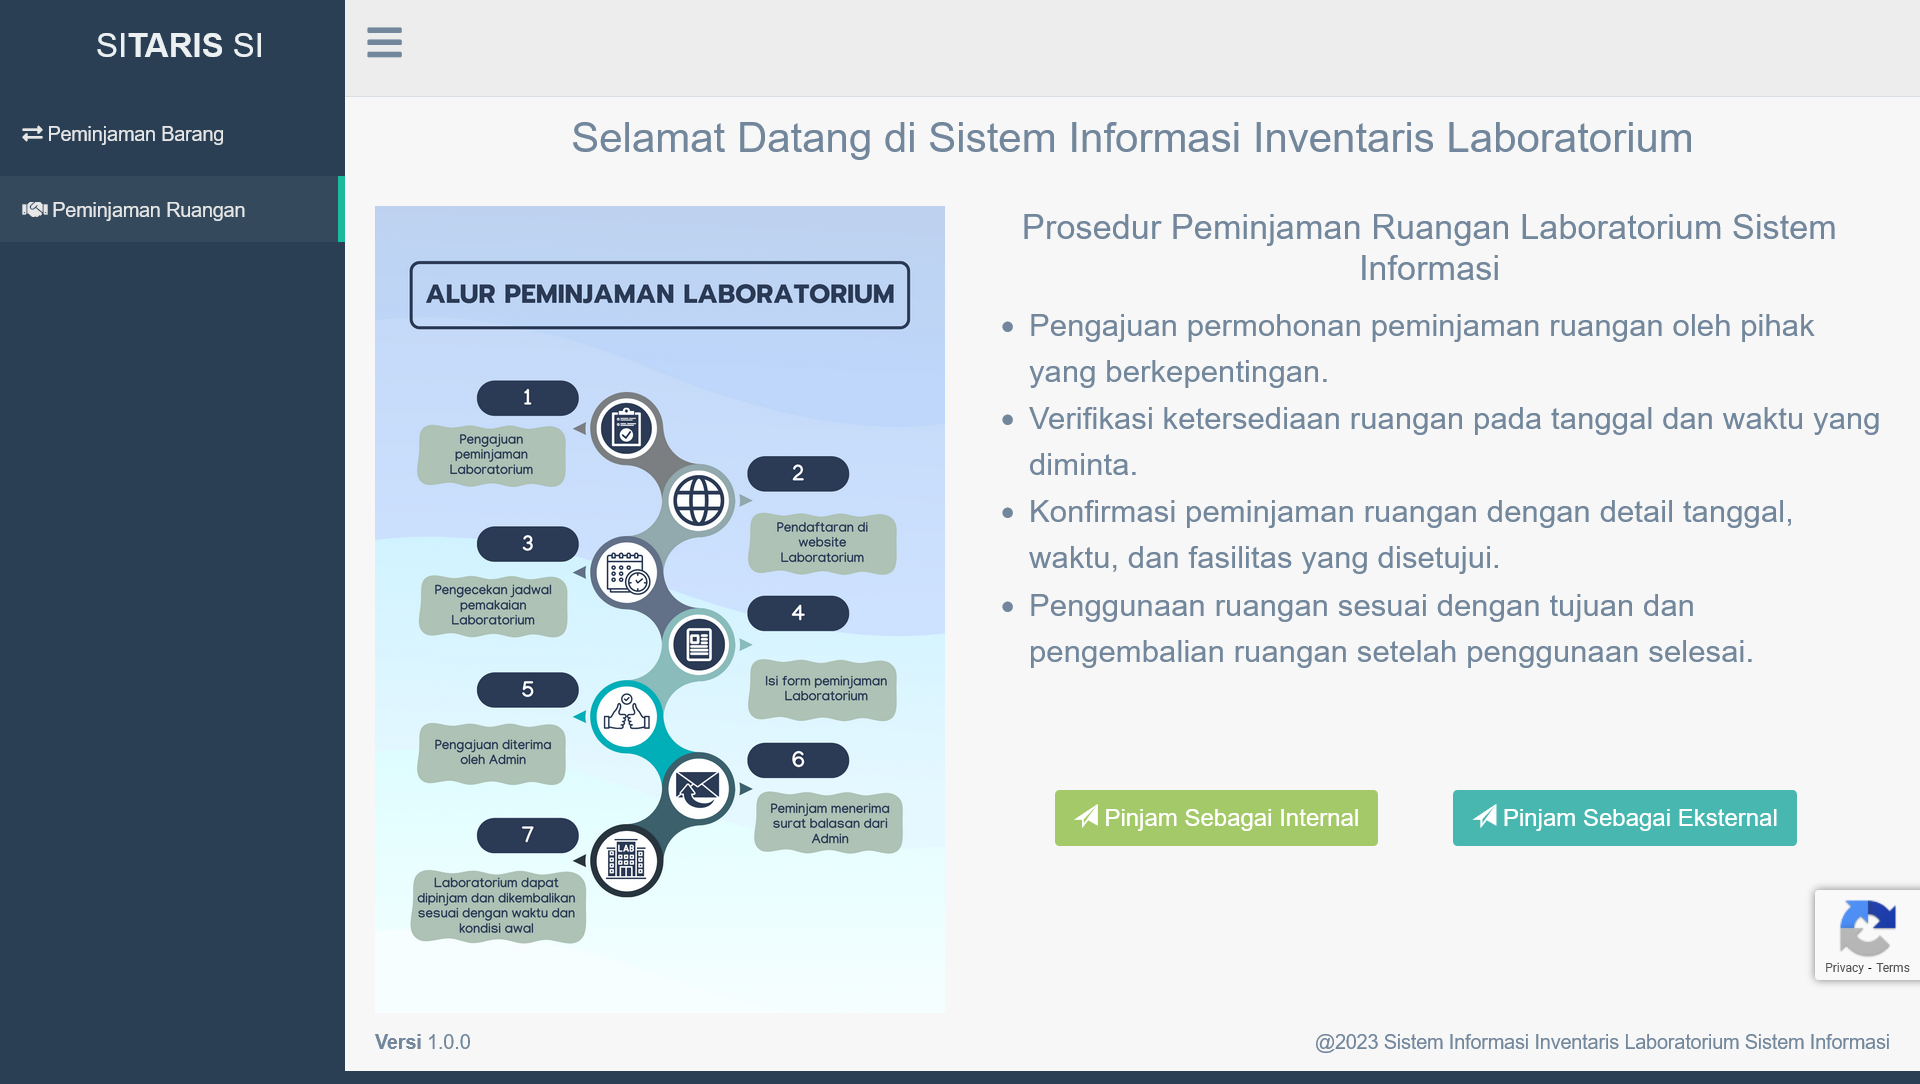
\includegraphics[width=0.82\linewidth]{konten//gambar/peminjaman ruangan peminjam.png}
          \caption{Halaman Peminjaman Ruangan Bagi Peminjam}
          \label{fig:enter-label}
        \end{figure}

        \begin{figure}
          \centering
          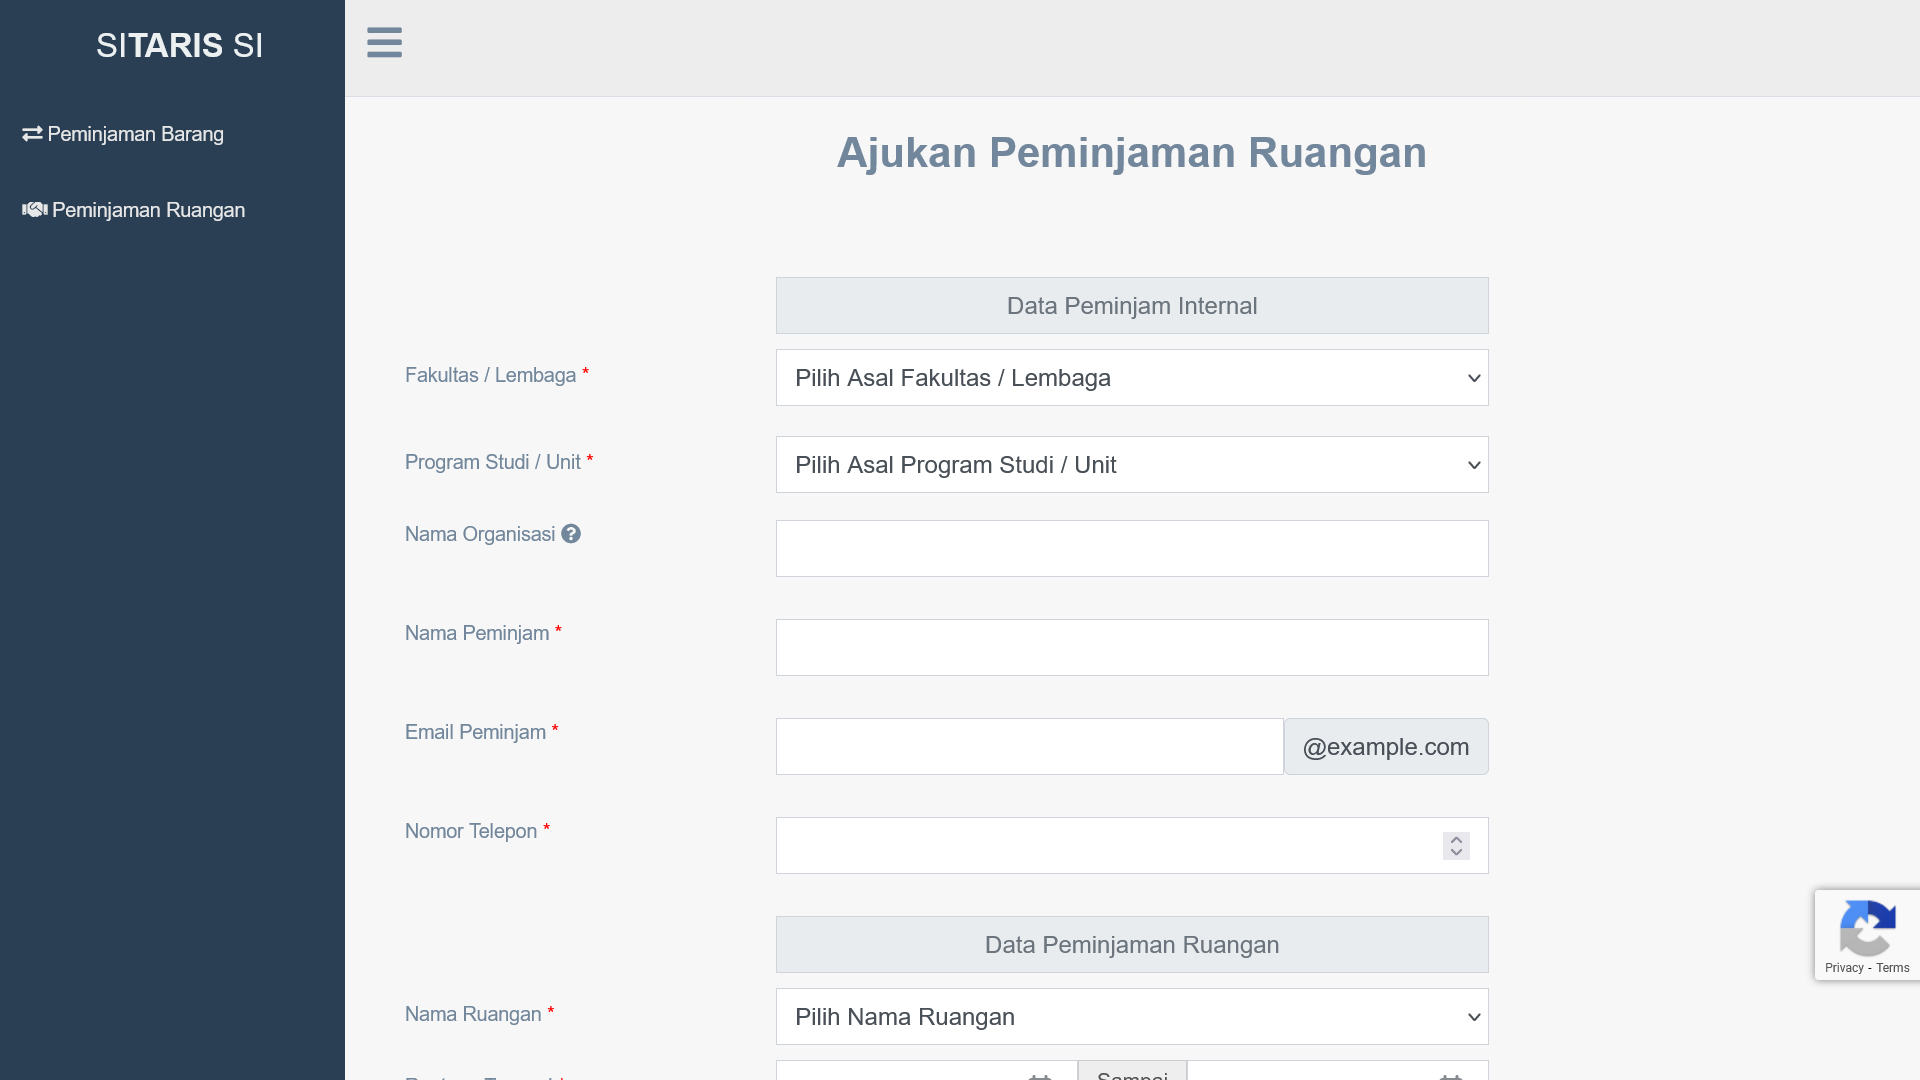
\includegraphics[width=0.82\linewidth]{konten//gambar/peminjaman ruangan tambah internal.png}
          \caption{Halaman Peminjaman Ruangan Bagi Peminjam Internal}
          \label{fig:enter-label}
        \end{figure}

        \begin{figure}
          \centering
          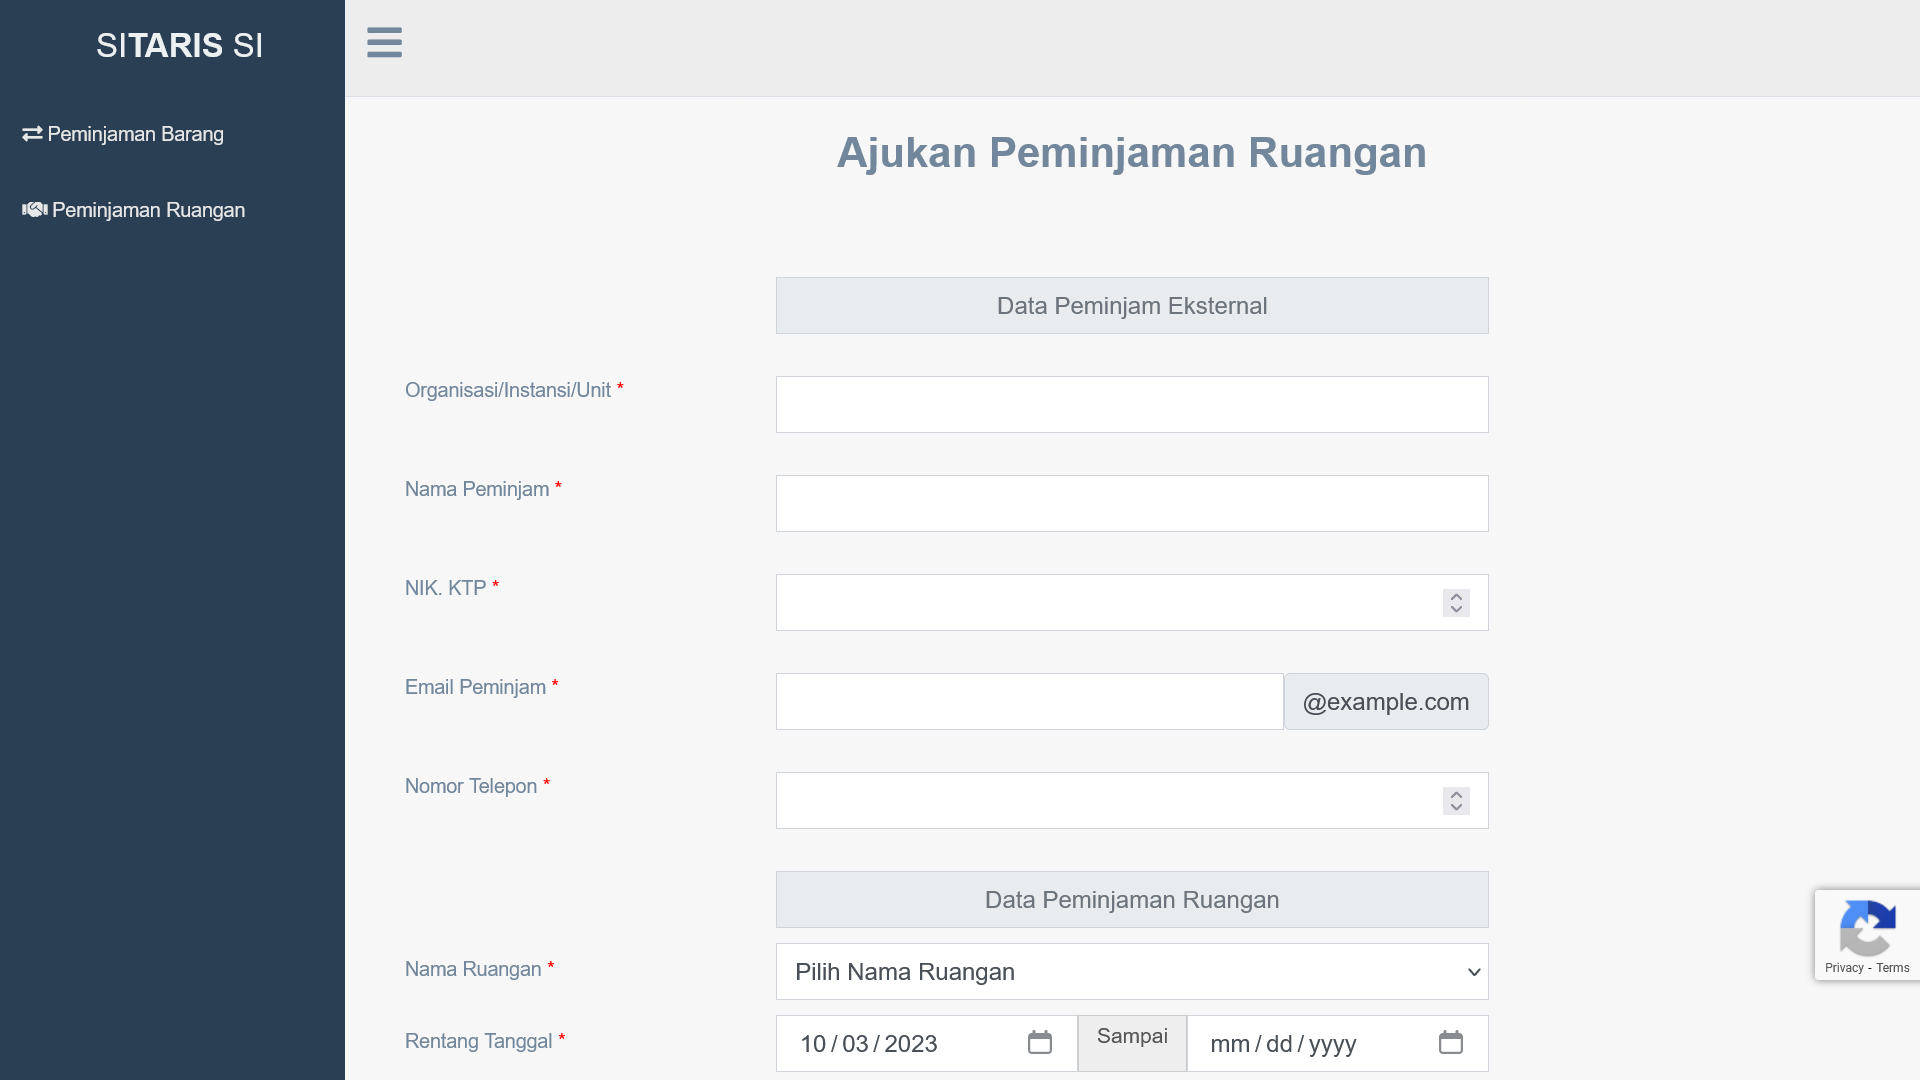
\includegraphics[width=0.82\linewidth]{konten//gambar/peminjaman ruangan tambah eksternal.png}
          \caption{Halaman Peminjaman Ruangan Bagi Peminjam Eksternal}
          \label{fig:enter-label}
        \end{figure}

  \item Halaman Dokumentasi \\ Halaman dokumentasi merupakan tampilan untuk melihat dan mengelola data dokumentasi, tombol tambah data merupakan tombol yang dapat digunakan untuk beralih ke halaman tambah data dokumentasi, dan tombol pensil digunakan untuk mengedit data dokumentasi dan tombol \textit{trash} untuk menghapus data dokumentasi seperti pada Gambar 2.36. sampai Gambar 2.40.

        \begin{figure}
          \centering
          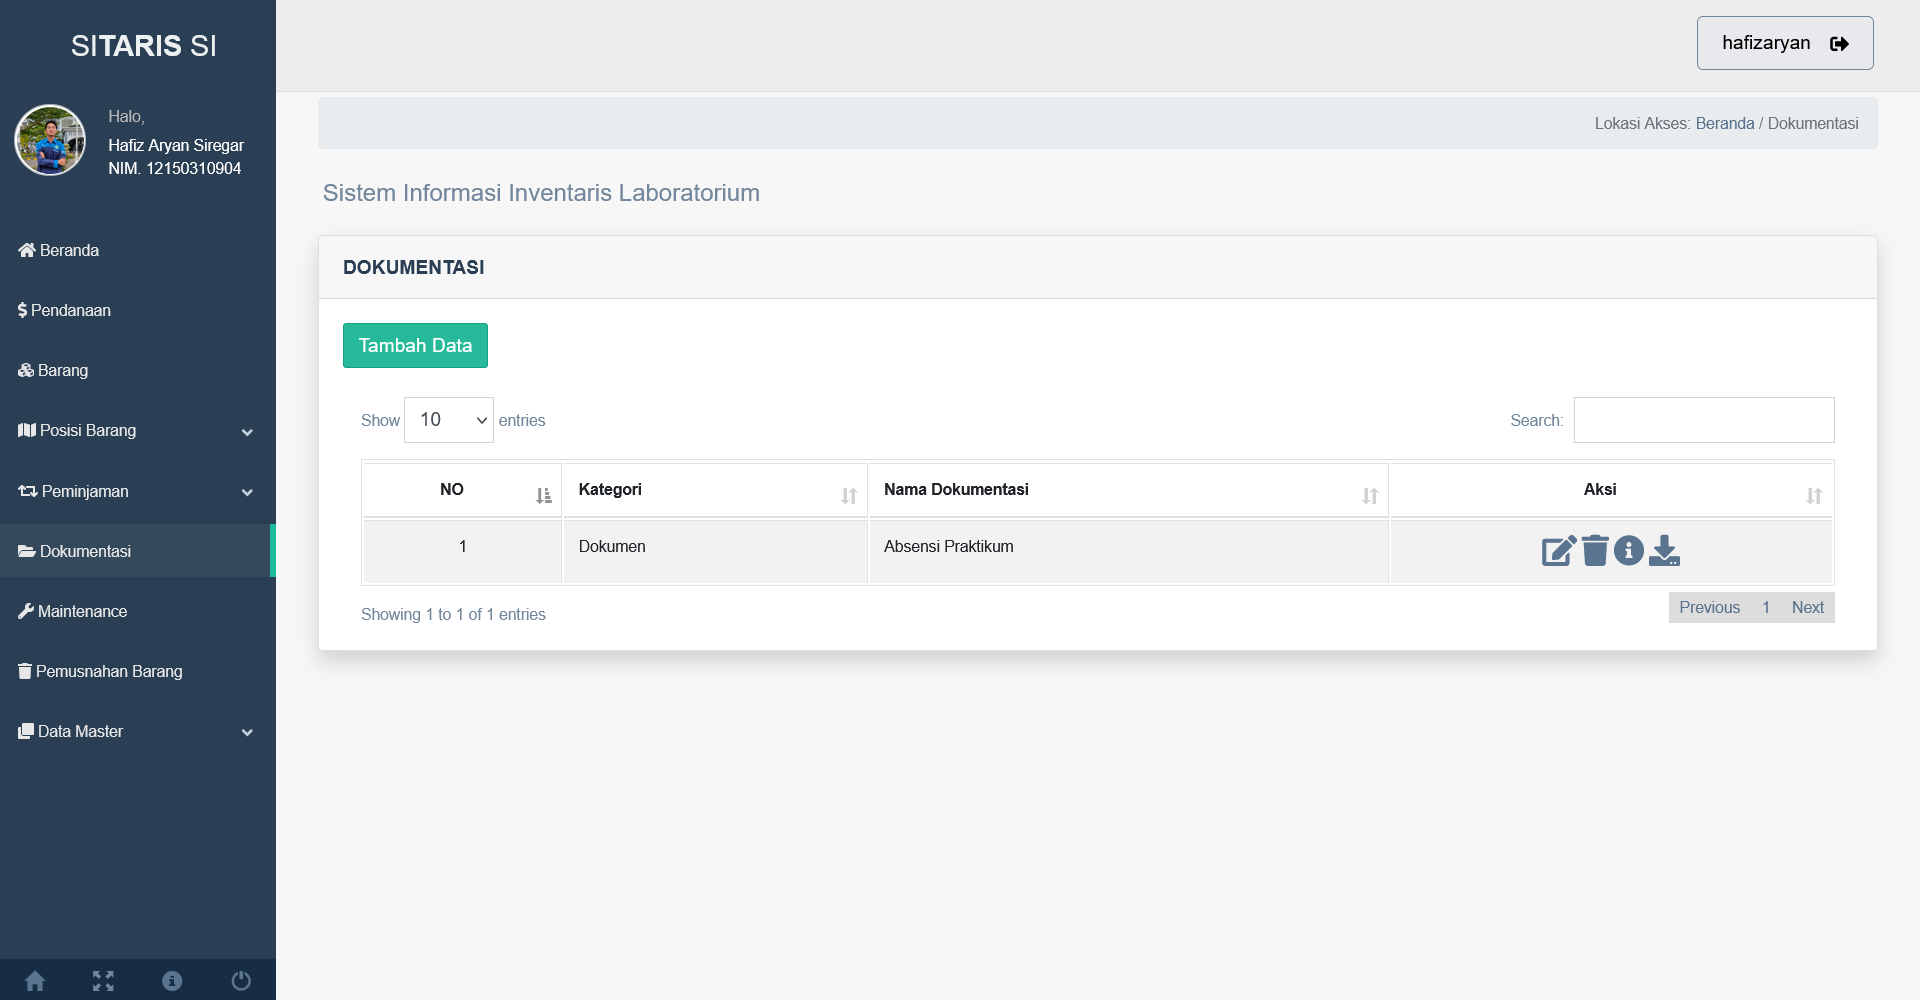
\includegraphics[width=0.82\linewidth]{konten//gambar/dokumentasi index.png}
          \caption{Halaman Dokumentasi \textit{Index}}
          \label{fig:enter-label}
        \end{figure}

        \begin{figure}
          \centering
          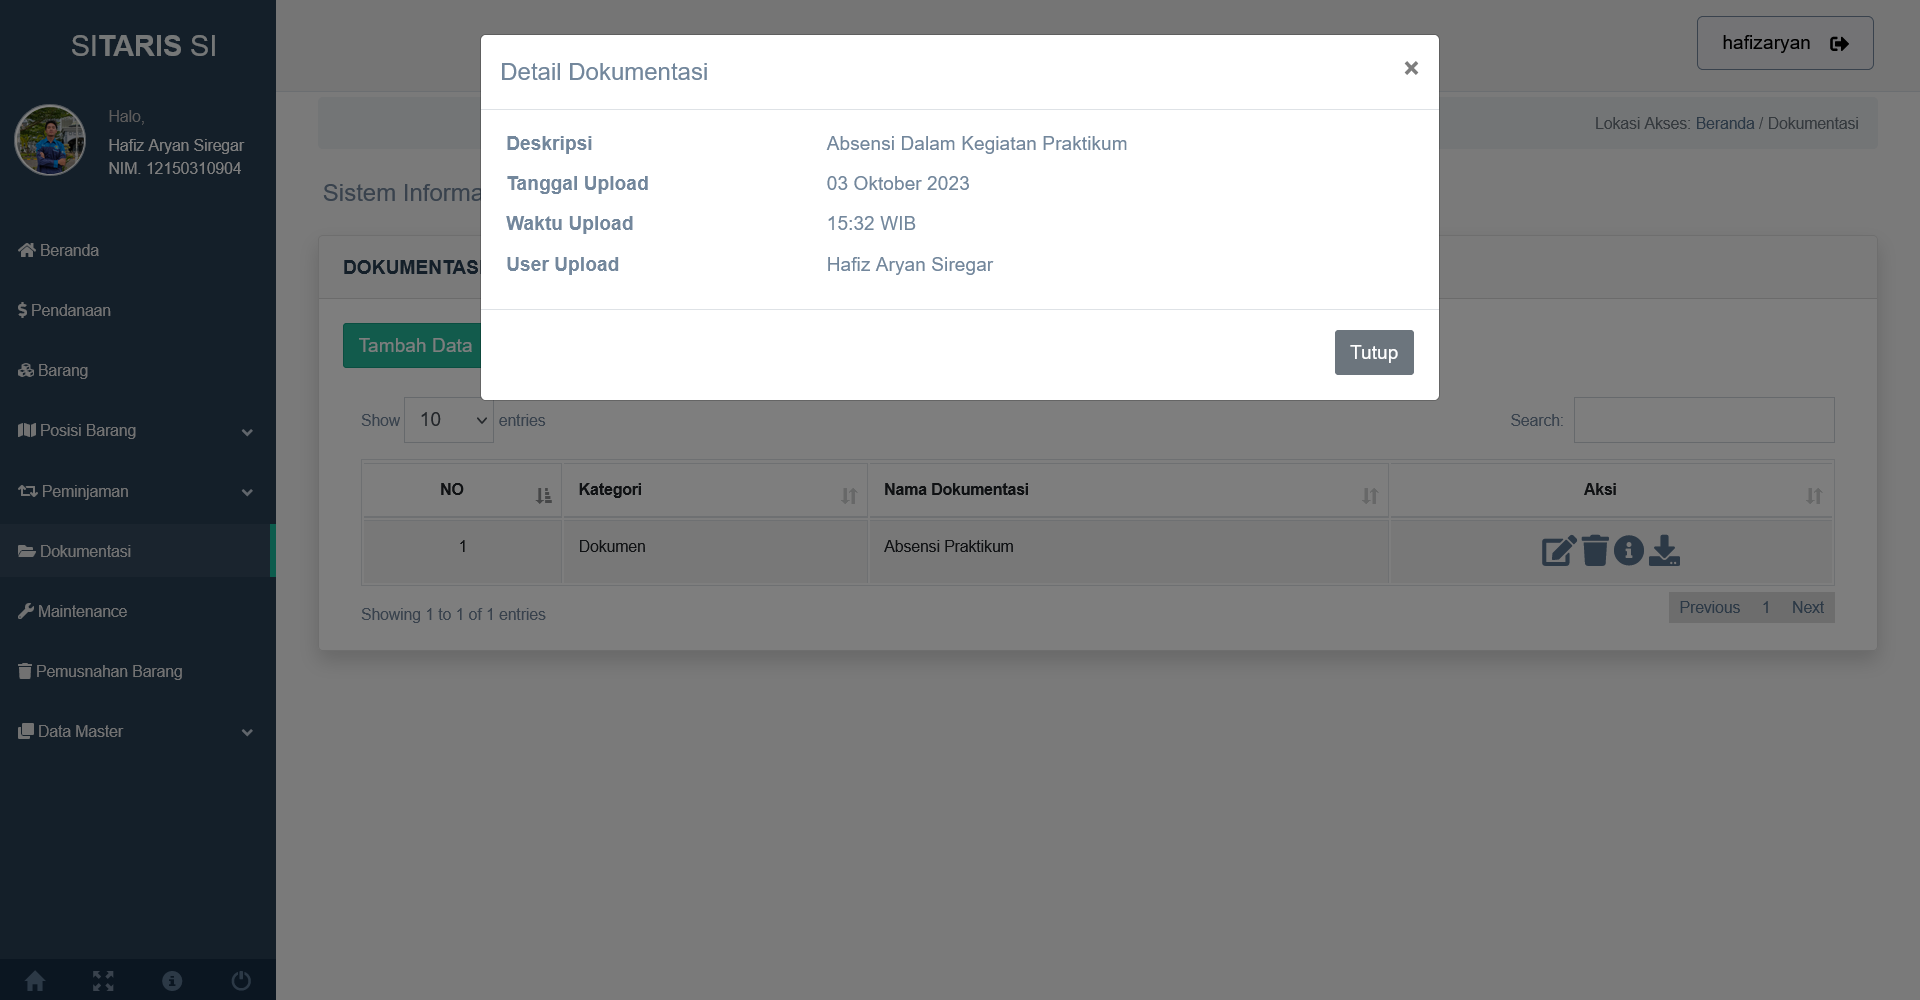
\includegraphics[width=0.82\linewidth]{konten//gambar/dokumentasi detail.png}
          \caption{Tampilan Detail Dokumentasi}
          \label{fig:enter-label}
        \end{figure}

        \begin{figure}
          \centering
          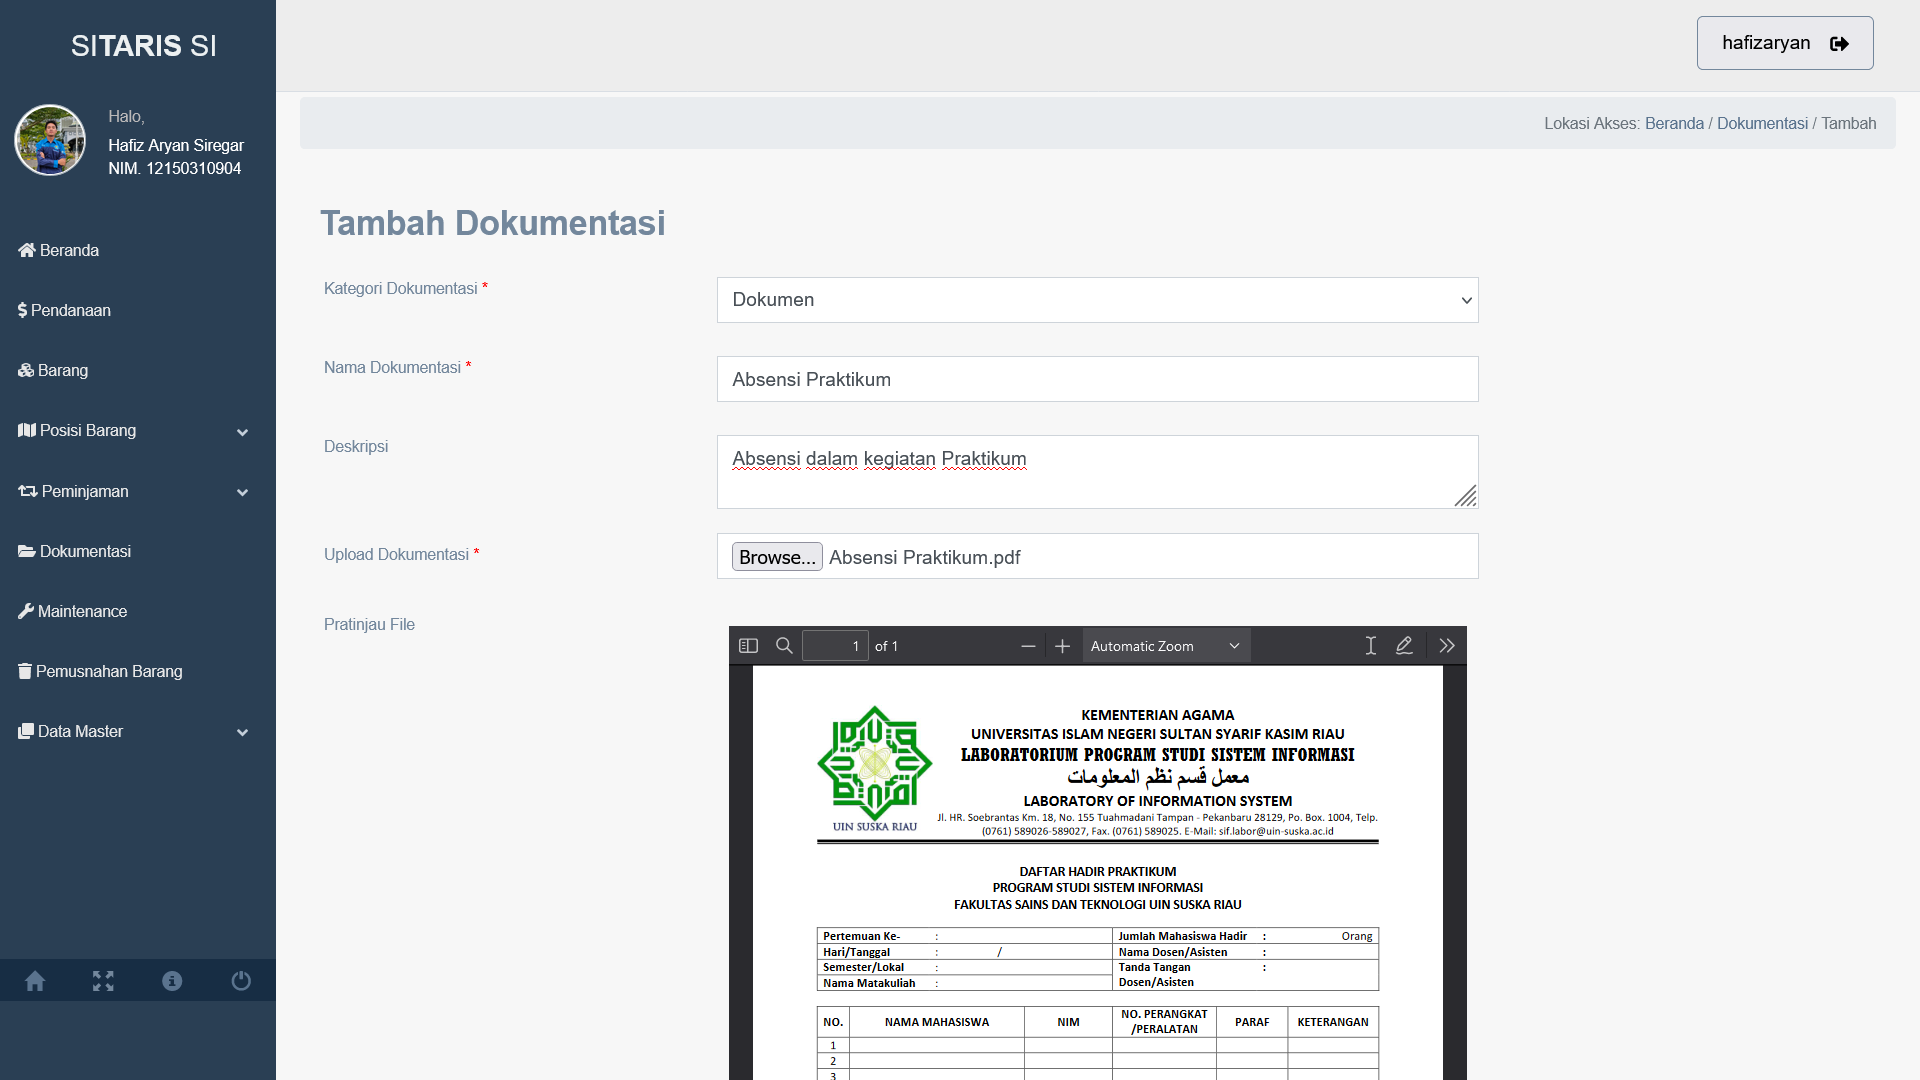
\includegraphics[width=0.82\linewidth]{konten//gambar/dokumentasi tambah.png}
          \caption{Halaman Tambah Dokumentasi}
          \label{fig:enter-label}
        \end{figure}

        \begin{figure}
          \centering
          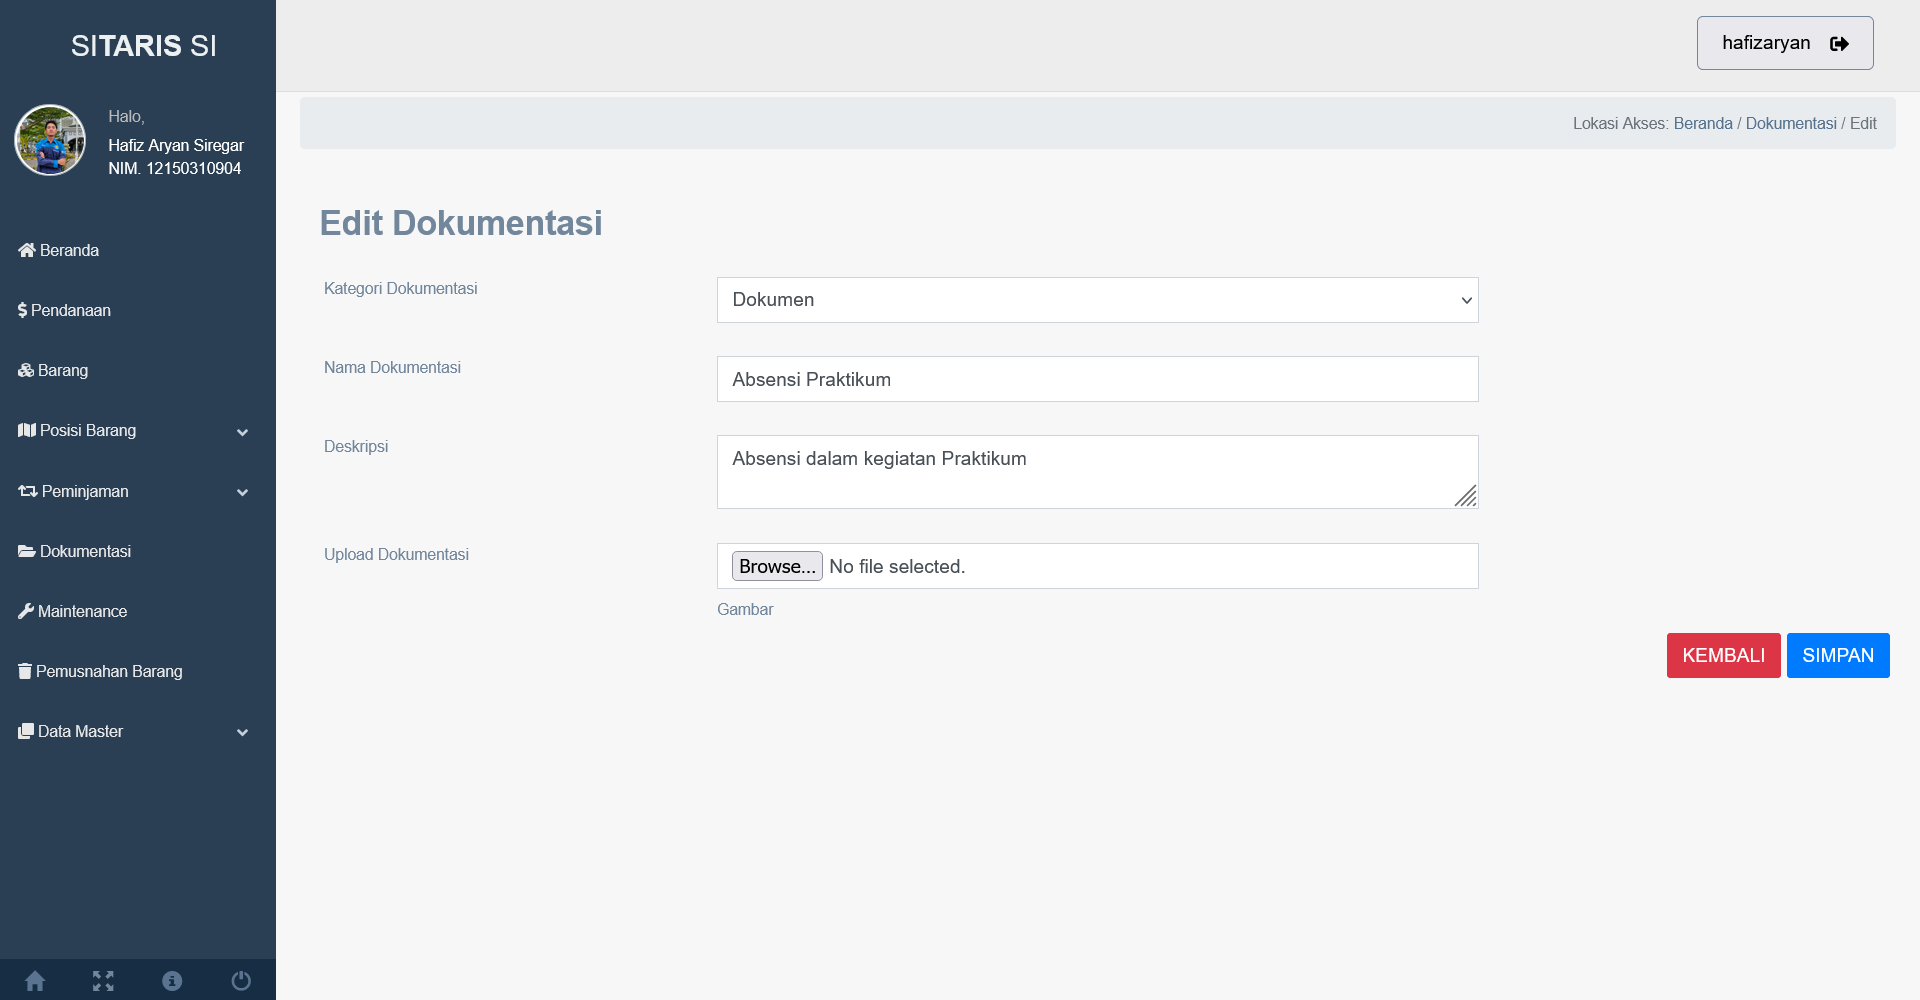
\includegraphics[width=0.82\linewidth]{konten//gambar/dokumentasi edit.png}
          \caption{Halaman Edit Dokumentasi}
          \label{fig:enter-label}
        \end{figure}

        \begin{figure}
          \centering
          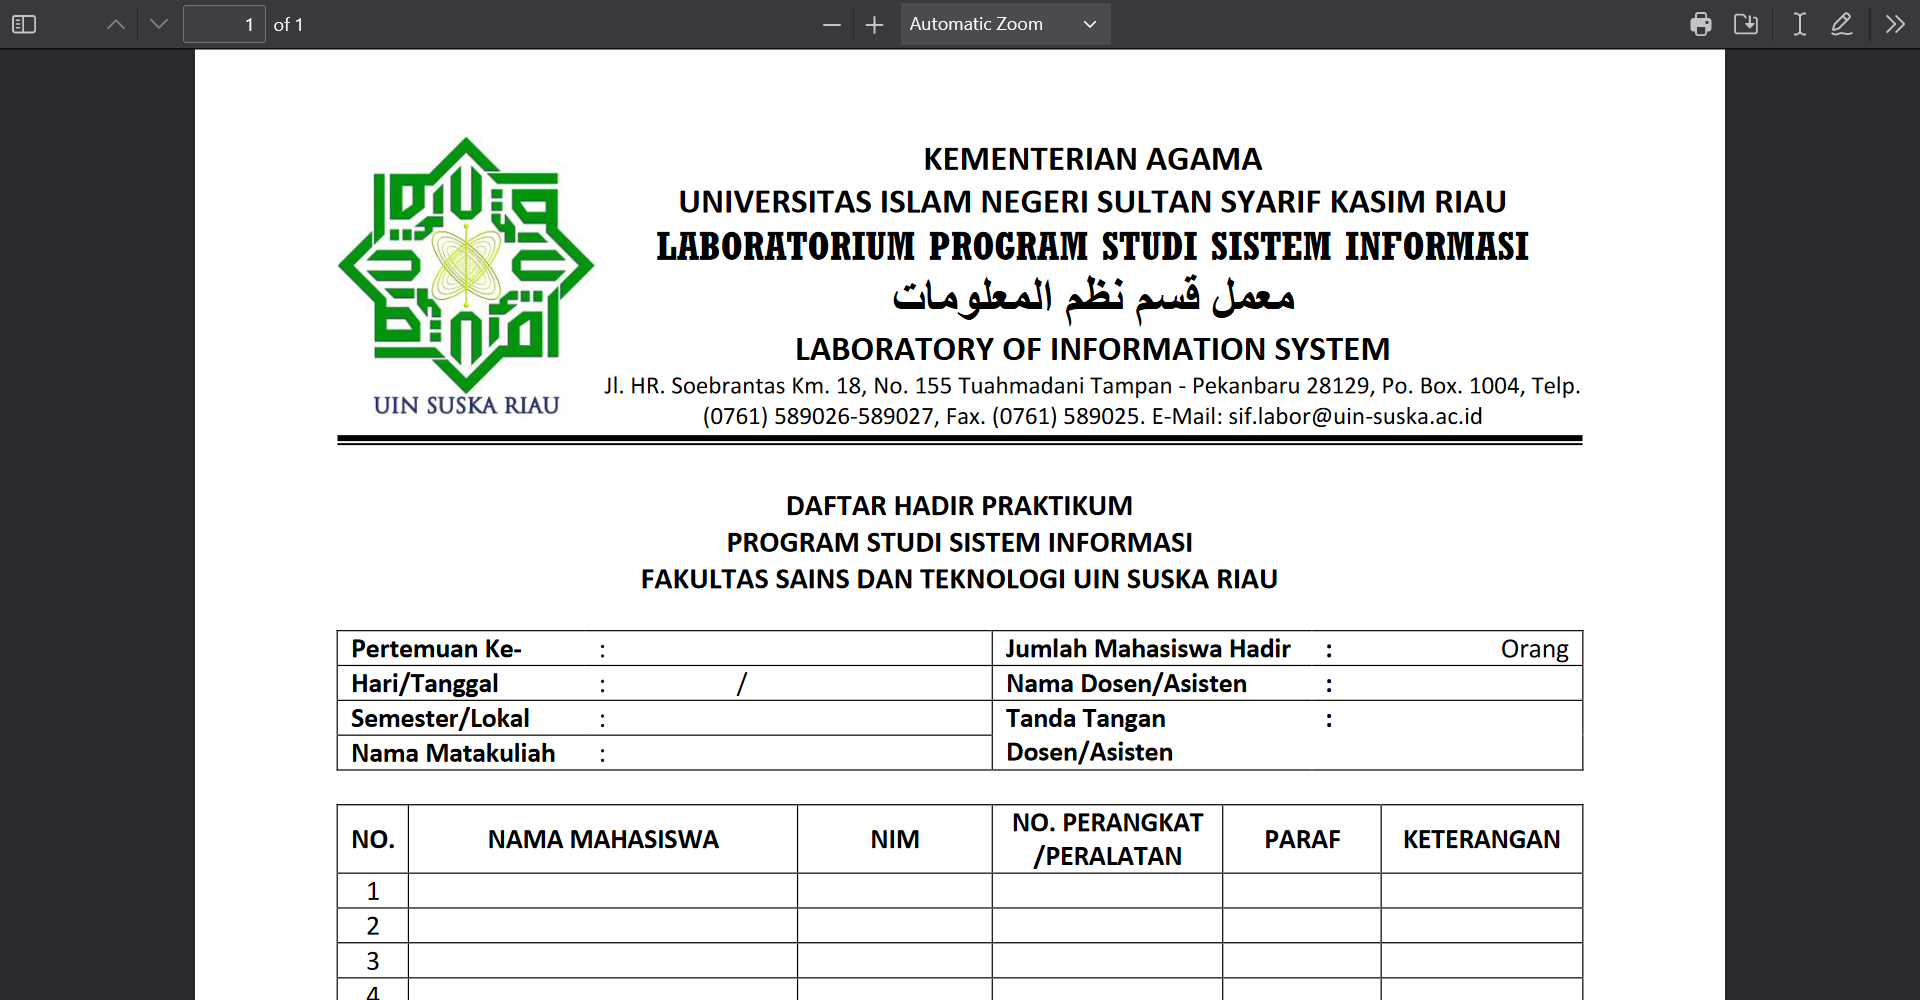
\includegraphics[width=0.82\linewidth]{konten//gambar/dokumentasi download.png}
          \caption{Halaman Download Dokumentasi}
          \label{fig:enter-label}
        \end{figure}

  \item Halaman \textit{Maintenance} \\ Halaman \textit{maintenance} merupakan tampilan untuk melihat dan mengelola data \textit{maintenance}, tombol tambah data merupakan tombol yang dapat digunakan untuk beralih ke halaman tambah data \textit{maintenance}, dan tombol pensil digunakan untuk mengedit data \textit{maintenance} dan tombol \textit{trash} untuk menghapus data \textit{maintenance} seperti pada Gambar 2.41. sampai Gambar 2.44.
        \begin{figure}
          \centering
          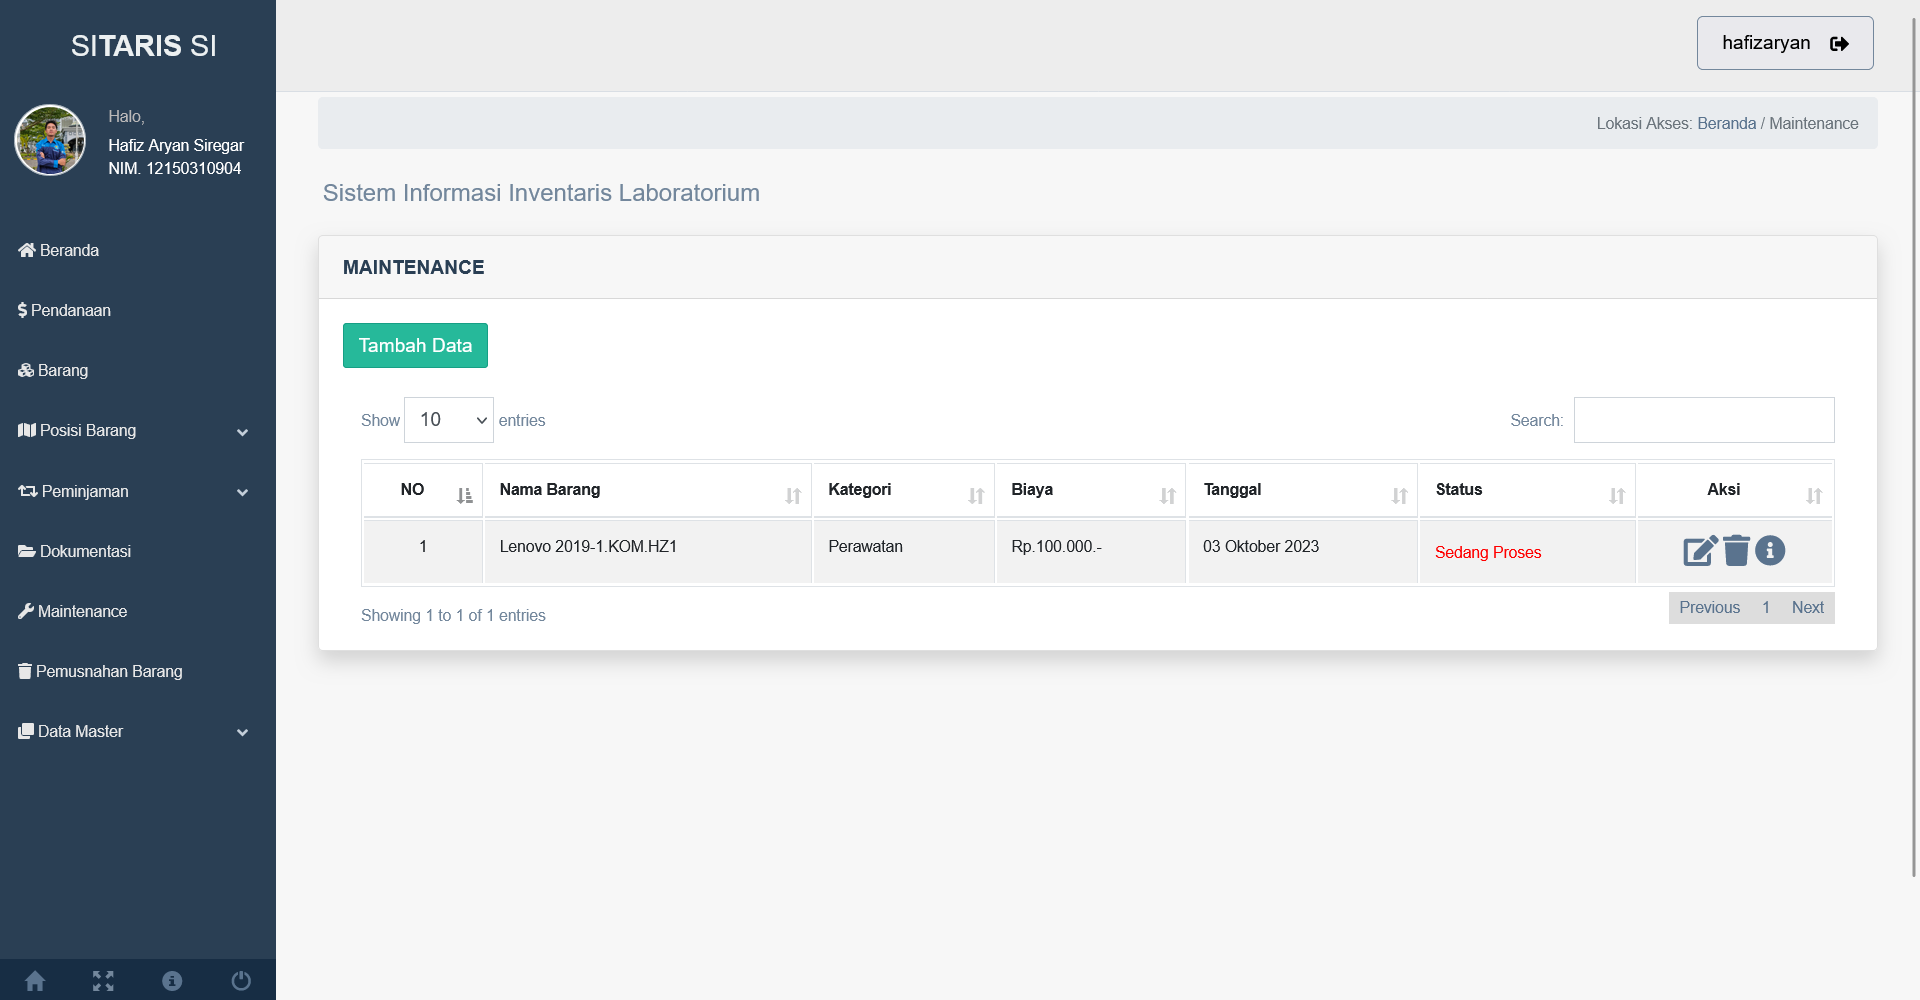
\includegraphics[width=0.82\linewidth]{konten//gambar/maintenance index.png}
          \caption{Halaman \textit{Maintenance} \textit{Index}}
          \label{fig:enter-label}
        \end{figure}

        \begin{figure}
          \centering
          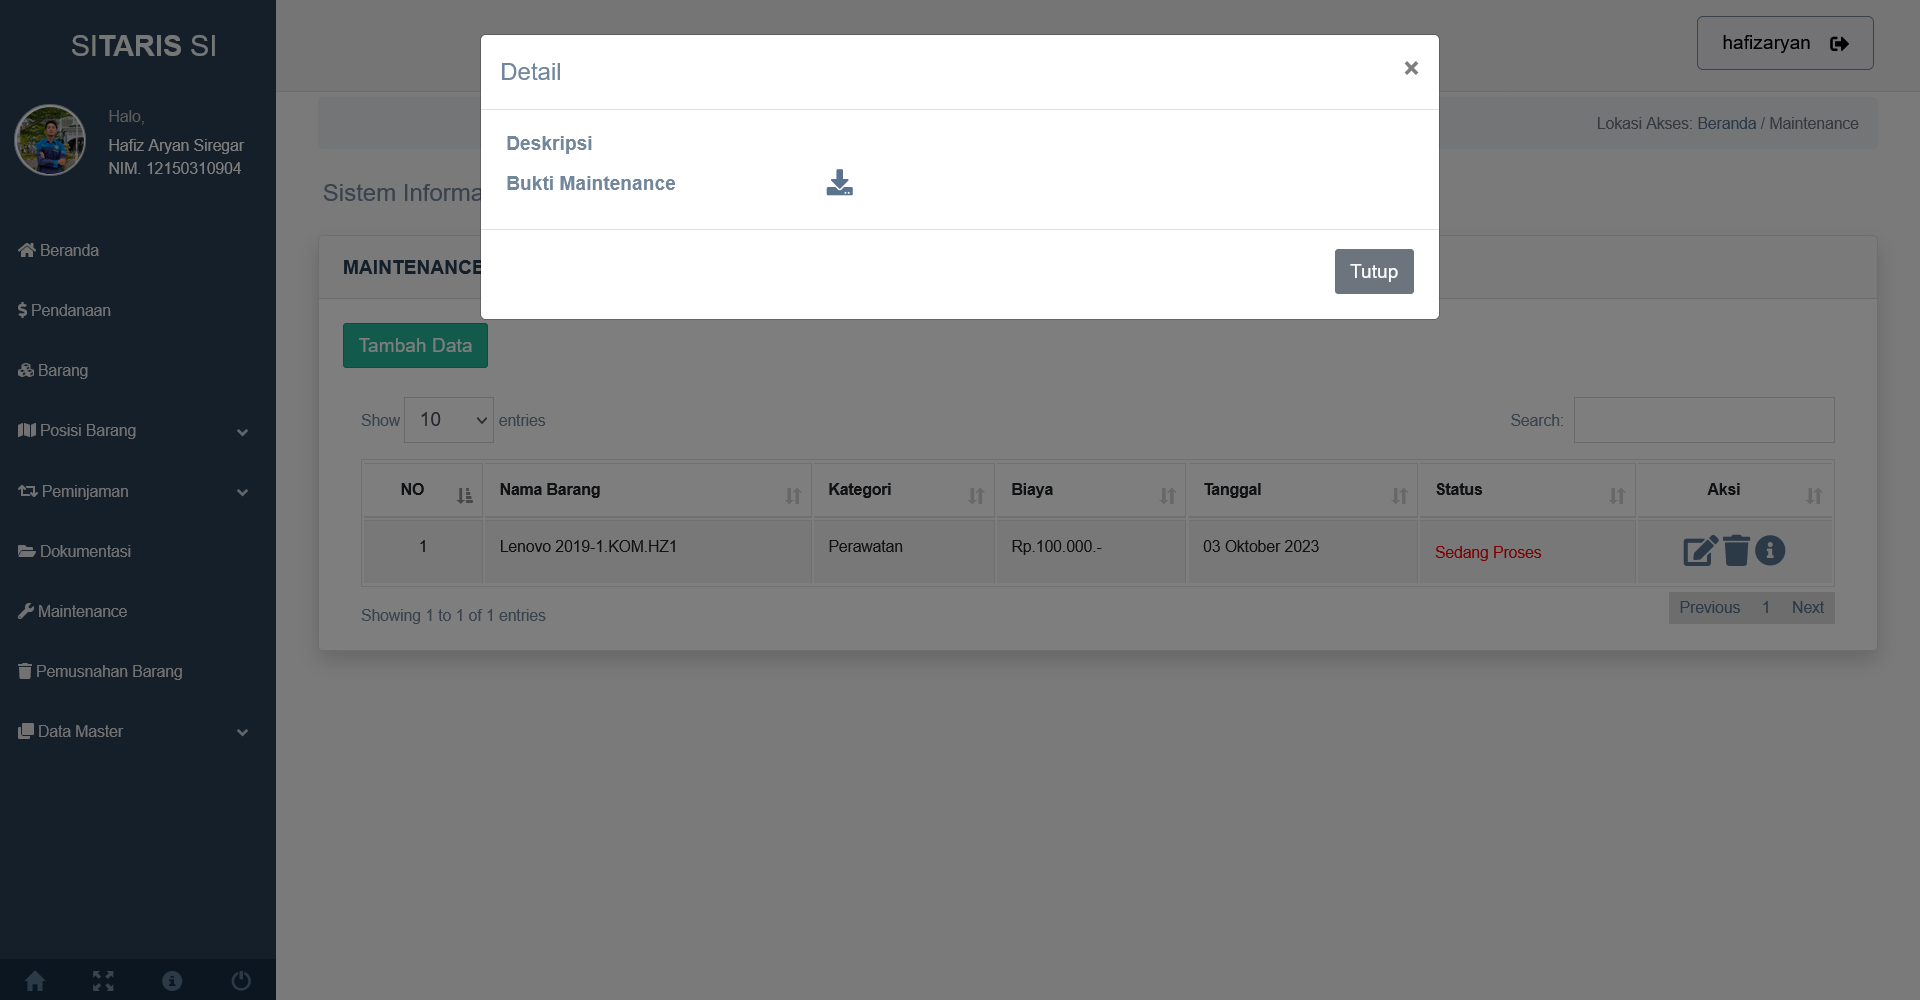
\includegraphics[width=0.82\linewidth]{konten//gambar/maintenance detail.png}
          \caption{Tampilan Detail \textit{Maintenance}}
          \label{fig:enter-label}
        \end{figure}

        \begin{figure}
          \centering
          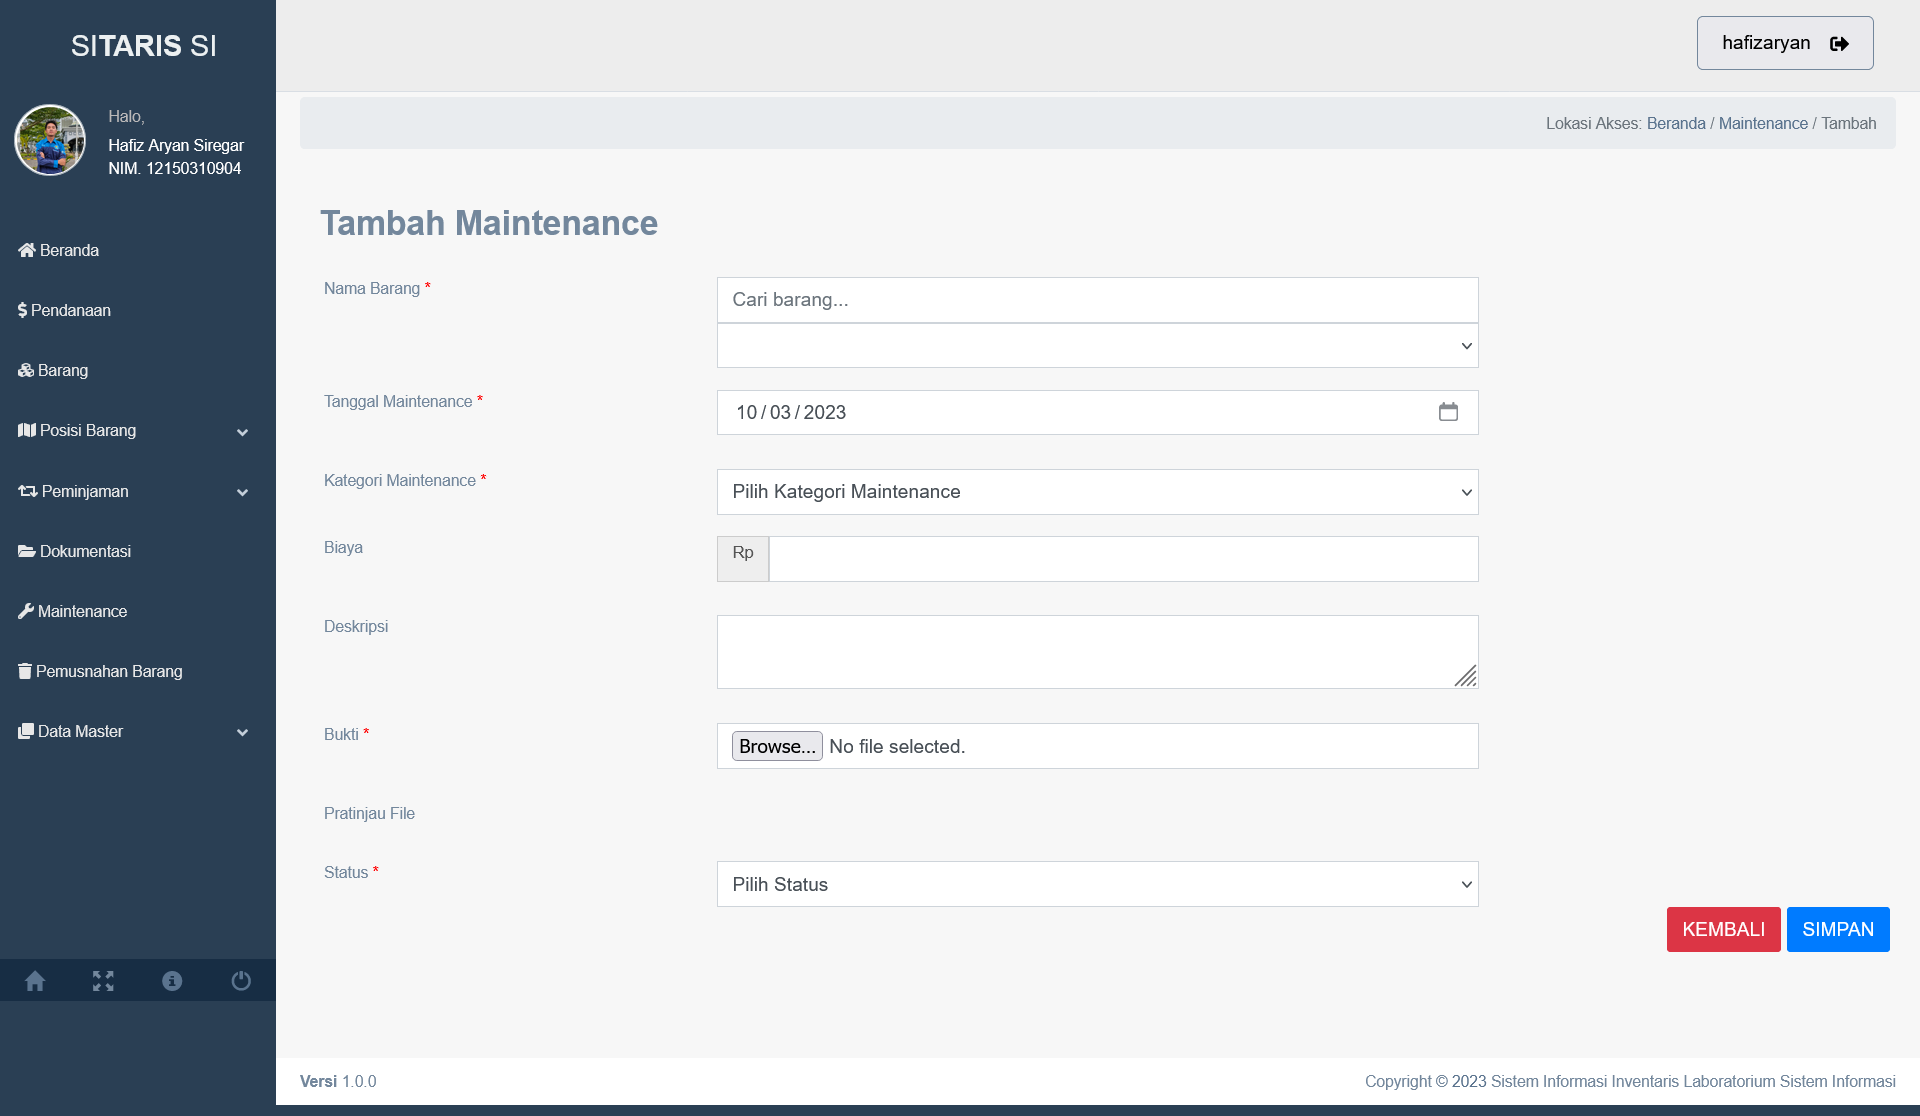
\includegraphics[width=0.82\linewidth]{konten//gambar/maintenance tambah.png}
          \caption{Halaman Tambah \textit{Maintenance}}
          \label{fig:enter-label}
        \end{figure}

        \begin{figure}
          \centering
          \includegraphics[width=0.82\linewidth]{konten//gambar/maintenance edit.png}
          \caption{Halaman Edit \textit{Maintenance}}
          \label{fig:enter-label}
        \end{figure}

  \item Halaman Pemusnahan Barang \\ Halaman pemusnahan barang merupakan tampilan untuk melihat dan mengelola data pemusnahan barang, tombol tambah data merupakan tombol yang dapat digunakan untuk beralih ke halaman tambah data pemusnahan barang, dan tombol pensil digunakan untuk mengedit data pemusnahan barang dan tombol \textit{trash} untuk menghapus data pemusnahan barang seperti pada Gambar 2.45. sampai Gambar 2.48.

        \begin{figure}
          \centering
          \includegraphics[width=0.82\linewidth]{konten//gambar/pemusnahan barang index.png}
          \caption{Halaman Pemusnahan Barang \textit{Index}}
          \label{fig:enter-label}
        \end{figure}

        \begin{figure}
          \centering
          \includegraphics[width=0.82\linewidth]{konten//gambar/pemusnahan barangdtl.png}
          \caption{Tampilan Detail Pemusnahan Barang}
          \label{fig:enter-label}
        \end{figure}

        \begin{figure}
          \centering
          \includegraphics[width=0.82\linewidth]{konten//gambar/pemusnahan barangtbh.png}
          \caption{Halaman Tambah Pemusnahan Barang}
          \label{fig:enter-label}
        \end{figure}

        \begin{figure}
          \centering
          \includegraphics[width=0.82\linewidth]{konten//gambar/pemusnahan barang edit.png}
          \caption{Halaman Edit Pemusnahan Barang}
          \label{fig:enter-label}
        \end{figure}

  \item Halaman Fakultas \\ Halaman fakultas merupakan tampilan untuk melihat dan mengelola data fakultas, tombol tambah data merupakan tombol yang dapat digunakan untuk beralih ke halaman tambah data fakultas, dan tombol pensil digunakan untuk mengedit data fakultas dan tombol \textit{trash} untuk menghapus data fakultas seperti pada Gambar 2.49. sampai Gambar 2.51.

        \begin{figure}
          \centering
          \includegraphics[width=0.82\linewidth]{konten//gambar/fakultas index.png}
          \caption{Halaman Fakultas \textit{Index}}
          \label{fig:enter-label}
        \end{figure}

        \begin{figure}
          \centering
          \includegraphics[width=0.82\linewidth]{konten//gambar/fakultas tambah.png}
          \caption{Halaman Tambah Fakultas}
          \label{fig:enter-label}
        \end{figure}

        \begin{figure}
          \centering
          \includegraphics[width=0.82\linewidth]{konten//gambar/fakultas edit.png}
          \caption{Halaman Edit Fakultas}
          \label{fig:enter-label}
        \end{figure}

  \item Halaman Prodi \\ Halaman prodi merupakan tampilan untuk melihat dan mengelola data prodi, tombol tambah data merupakan tombol yang dapat digunakan untuk beralih ke halaman tambah data prodi, dan tombol pensil digunakan untuk mengedit data prodi dan tombol \textit{trash} untuk menghapus data prodi seperti pada Gambar 2.52. sampai Gambar 2.54.

        \begin{figure}
          \centering
          \includegraphics[width=0.82\linewidth]{konten//gambar/prodi index.png}
          \caption{Halaman Prodi Index}
          \label{fig:enter-label}
        \end{figure}

        \begin{figure}
          \centering
          \includegraphics[width=0.82\linewidth]{konten//gambar/prodi tambah.png}
          \caption{Halaman Tambah Prodi}
          \label{fig:enter-label}
        \end{figure}

        \begin{figure}
          \centering
          \includegraphics[width=0.82\linewidth]{konten//gambar/prodi edit.png}
          \caption{Halaman Edit Prodi}
          \label{fig:enter-label}
        \end{figure}

  \item Halaman Gedung \\ Halaman gedung merupakan tampilan untuk melihat dan mengelola data gedung, tombol tambah data merupakan tombol yang dapat digunakan untuk beralih ke halaman tambah data gedung, dan tombol pensil digunakan untuk mengedit data gedung dan tombol \textit{trash} untuk menghapus data gedung seperti pada Gambar 2.55. sampai Gambar 2.57.
        \begin{figure}
          \centering
          \includegraphics[width=0.82\linewidth]{konten//gambar/gedung index.png}
          \caption{Halaman Gedung \textit{Index}}
          \label{fig:enter-label}
        \end{figure}

        \begin{figure}
          \centering
          \includegraphics[width=0.82\linewidth]{konten//gambar/gedung tambah.png}
          \caption{Halaman Tambah Gedung}
          \label{fig:enter-label}
        \end{figure}

        \begin{figure}
          \centering
          \includegraphics[width=0.82\linewidth]{konten//gambar/gedung edit.png}
          \caption{Halaman Edit Gedung}
          \label{fig:enter-label}
        \end{figure}

  \item Halaman Ruangan \\ Halaman ruangan merupakan tampilan untuk melihat dan mengelola data ruangan, tombol tambah data merupakan tombol yang dapat digunakan untuk beralih ke halaman tambah data ruangan, dan tombol pensil digunakan untuk mengedit data ruangan dan tombol \textit{trash} untuk menghapus data ruangan seperti pada Gambar 2.58. sampai Gambar 2.60.
        \begin{figure}
          \centering
          \includegraphics[width=0.82\linewidth]{konten//gambar/ruangan index.png}
          \caption{Halaman Ruangan \textit{Index}}
          \label{fig:enter-label}
        \end{figure}

        \begin{figure}
          \centering
          \includegraphics[width=0.82\linewidth]{konten//gambar/ruangan tambah.png}
          \caption{Halaman Tambah Ruangan}
          \label{fig:enter-label}
        \end{figure}

        \begin{figure}
          \centering
          \includegraphics[width=0.82\linewidth]{konten//gambar/ruangan edit.png}
          \caption{Halaman Edit Ruangan}
          \label{fig:enter-label}
        \end{figure}

  \item Halaman Pengguna \\ Halaman pengguna merupakan tampilan untuk melihat dan mengelola data pengguna, tombol tambah data merupakan tombol yang dapat digunakan untuk beralih ke halaman tambah data pengguna, dan tombol pensil digunakan untuk mengedit data pengguna dan tombol \textit{trash} untuk menghapus data pengguna seperti pada Gambar 2.61. sampai Gambar 2.64.

        \begin{figure}
          \centering
          \includegraphics[width=0.82\linewidth]{konten//gambar/user index.png}
          \caption{Halaman Pengguna \textit{Index}}
          \label{fig:enter-label}
        \end{figure}

        \begin{figure}
          \centering
          \includegraphics[width=0.82\linewidth]{konten//gambar/user detail.png}
          \caption{Tampilan Detail Pengguna}
          \label{fig:enter-label}
        \end{figure}

        \begin{figure}
          \centering
          \includegraphics[width=0.82\linewidth]{konten//gambar/user tambah.png}
          \caption{Halaman Tambah Pengguna}
          \label{fig:enter-label}
        \end{figure}

        \begin{figure}
          \centering
          \includegraphics[width=0.82\linewidth]{konten//gambar/user edit.png}
          \caption{Halaman Edit Pengguna}
          \label{fig:enter-label}
        \end{figure}

  \item Halaman Profil \\ Halaman profil merupakan tampilan untuk melihat dan mengelola data profil, tombol edit profil merupakan tombol yang dapat digunakan untuk beralih ke halaman tambah edit profil seperti pada Gambar 2.65. sampai Gambar 2.66.

        \begin{figure}
          \centering
          \includegraphics[width=0.82\linewidth]{konten//gambar/profil.png}
          \caption{Halaman Profil Pengguna}
          \label{fig:enter-label}
        \end{figure}

        \begin{figure}
          \centering
          \includegraphics[width=0.82\linewidth]{konten//gambar/profil edit.png}
          \caption{Halaman Edit Profil Pengguna}
          \label{fig:enter-label}
        \end{figure}

  \item Halaman Pengembang \\ Halaman pengembang merupakan tampilan untuk melihat data pengembang seperti pada Gambar 2.67.

        \begin{figure}
          \centering
          \includegraphics[width=0.82\linewidth]{konten//gambar/pengembang.png}
          \caption{Halaman Pengembang}
          \label{fig:enter-label}
        \end{figure}

\end{enumerate}


\section{Evaluasi}
Salah satu komponen penting dari penilaian organisasi adalah evaluasi, yang didefinisikan sebagai proses menilai seberapa efektif startegi yang digunakan untuk mencapai tujuan organisasi \cite{al2018evaluasi}. Adapun tujuan dan fungsi dari evaluasi yaitu, untuk mengetahui apakah tujuan-tujuan yang telah ditetapkan telah tercapai dalam kegiatan, untuk memberikan objektivitas pengamatan terhadap perilaku hasil, un tuk mengetahui kemampuan dan menentukan kelayakan, dan untuk memberikan umpan balik bagi kegiatan yang dilakukan. Evaluasi dilakukan sebagai uji coba untuk melihat sejauh apa sebuah software dapat dikatakan berkualitas dan sebagai acuan untuk melakukan pengembangan software. Perlunya dilakukan evaluasi agar dapat men gukur fungsionalitas dari portal akademik. Hasil dari evaluasi dapat menyimpulkan 20 fungsi/proses apa yang sudah berjalan dengan baik dan yang belum/tidak berjalan dengan baik \cite{terttiaavini2014analisa}.

\subsection{Prosedur Evaluasi}
Proses suatu evaluasi pada umumnya memilik tahapan-tahapannya sendiri. Walaupun tidak selalu sama, tetapi yang lebih penting adalah bahwa prosesnya sejalan dengan fungsi evaluasi itu sendiri. Berikut ini di paparkan salah satu tahapan evaluasi yang sifatnya umum digunakan. 

\begin{enumerate}
	\item Mengidentifikasi subjek yang akan dievaluasi. Apa pun yang dapat dievaluasi dapat dikaitkan dengan program kerja perusahaan. Banyak elemen yang kiranya dapat dan harus dievaluasi. Namun, hal-hal yang menjadi faktor penting keberhasilannya biasanya diberi prioritas untuk dievaluasi.
	\item Membuat kegiatan evaluasi. Sebelum memulai evaluasi, tentukan desain evaluasinya sehingga jelas data apa yang dibutuhkan, prosedur apa yang dilakukan, siapa yang akan terlibat, dan hasil apa yang akan dihasilkan.
	\item Pengumpulan data. Pengumpulan data dapat dilakukan secara efektif dan efisien sesuai dengan kebutuhan dan kemampuan, serta sesuai dengan kaidah ilmiah yang berlaku. Ini dapat dicapai berdasarkan desain yang telah disiapkan.
	\item Pengolahan dan pemeriksaan data Setelah data dikumpulkan. Data diproses untuk dikelompokkan dan dianalisis dengan menggunakan alat analisis yang sesuai untuk menghasilkan fakta yang dapat diandalkan. Selanjutnya, fakta dan harapan atau rencana dibandingkan untuk menemukan celah. Hasil dari evaluasi ini, lebar celah akan disesuaikan dengan tolok ukur tertentu.
	\item Pelaporan Hasil Evaluasi, Hasil evaluasi harus didokumentasikan secara tertulis dan diinformasikan baik secara lisan maupun tulisan agar pihak-pihak yang berkepentingan dapat menggunakannya.
	\item Tindak lanjut hasil penilaian. Sebagai bagian dari fungsi manajemen, evaluasi harus digunakan oleh manajemen untuk membuat keputusan tentang masalah manajemen di tingkat strategi dan implementasi.
\end{enumerate}

\subsection{Standar Evaluasi}
Standar yang dipakai untuk mengevaluasi suatu kegiatan tertentu dapat dilihat dari tiga aspek utama, yang menurut \textit{Committee on Standard for Educational Evaluation} kiranya dapat digunakan pula pada aspek bisnis, yaitu: 

\begin{enumerate}
	\item Manfaat (Utility). Hasil evaluasi harus membantu manajemen membuat keputusan tentang program yang sedang berjalan. Jika, misalnya, bagian dari suatu program promosi dievaluasi dan informasi yang dihasilkan dari evaluasi tidak membantu membuat keputusan, hasil evaluasi dianggap tidak bermanfaat.
	\item Akurat (Accuracy). Informasi tentang hasil evaluasi harus akurat. Misalnya, dalam program promosi, telah disepakati bahwa X rupiah akan digunakan untuk promosi sampai tengah tahun, dan Y kegiatan harus diselesaikan. Setelah evaluasi selesai, informasi harus dapat digunakan untuk menentukan apakah realisasi promosi dianggap menyimpang.
	\item  (Feasibility). Proses evaluasi yang direncanakan dapat dilak sanakan. Jika seseorang ingin menilai program promosi, mereka harus dapat melakukannya dengan baik dan benar dari sudut pandang teknis dan non-teknis, serta dari sudut pandang legal dan etis. Evaluasi yang memenuhi kriteria di atas adalah ideal dan tidak mudah dilaksanakan.
\end{enumerate}

\section{Kualitas Sistem}
Kualitas memiliki banyak aspek yang berbeda dan rumit. Kualitas sistem adalah istilah yang mengacu pada evaluasi proses sistem informasi dengan fokus pada hasil interaksi antara pengguna dan sistem. Kualitas sistem mencakup fitur seperti ketersediaan peralatan, keandalan peralatan, kemudahan penggunaan, dan waktu respons. Faktor-faktor ini adalah faktor penting yang menentukan apakah sistem informasi akan digunakan atau tidak \cite{pawirosumarto2016pengaruh}.

\section{Model ISO 9126}

\begin{figure}
  \centering
  \includegraphics[width=0.82\linewidth]{konten//gambar/Model-Iso.png}
  \caption{Karakteristik dan sub karakteristik ISO 9126}
  \label{fig:enter-label}
\end{figure}

ISO 9126 merupakan salah satu model atau \textit{framework} standar kualitas perangkat lunak yang diakui secara internasional berfungsi untuk melakukan pengujian kualitas pada perangkat lunak, yang dibuat oleh \textit{Internasional Organization for Standardization} (ISO) dan \textit{International Electrotechnical Commission (IEC)} yang diperkenalkan pada tahun 1991. Standar internasional dari ISO 9126 dapat mendefinisikan kualitas perangkat lunak, karakteristik mutu, model dan metrik yang terkait untuk mengevaluasi dan menetapkan kualitas sebuah produk perangkat lunak. Model ISO 9126 memiliki 6 (enam) aspek atau karakteristik, yaitu:  

\begin{enumerate}
	\item Fungsionalitas \textit{(functionality)}
	
	Fungsionalitas adalah kemampuan dalam perangkat lunak yang digunakan untuk penyediaan fungsi–fungsi yang memenuhi kebutuhan \textit{user} dengan dinyatakan atau tersirat. pada karakteristik ini, dapat dievaluasi melalui melalui fungsi dan layanan yang diberikan pada \textit{user}. Karakteristik ini terbagi atas beberapa sub karakteristik:

	\begin{enumerate}[label=\alph*)]
    \item \textit{Suitability}:
    
		Kemampuan perangkat lunak untuk menyediakan serangkaian fungsi yang sesuai untuk tugas-tugas tertentu dan tujuan pengguna.
    \item \textit{Accuracy}:
    
    Kemampuan perangkat lunak dalam memberikan hasil yang presisi atau akurat dan benar sesuai dengan kebutuhan.
    \item \textit{Security}:
    
		Kemampuan perangkat lunak untuk mencegah akses yang tidak
		diinginkan, menghadapi penyusup (\textit{hacker}) maupun otorisasi dalam modifikasi
		data. 
    \item \textit{Interoperability}:
    
    Kemampuan perangkat lunak untuk berinteraksi dengan satu atau lebih
		terhadap sistem tertentu atau sistem lainnya
	\end{enumerate}

	\item Kehandalan \textit{(reliabilty)}
	
	Reliabilitas merupakan kemampuan suatu produk perangkat lunak (\textit{software}) dalam mempertahankan tingkat kinerjanya pada kondisi tertentu yang telah ditetapkan pada periode waktu yang ditentukan. Pada karakteristik ini terdapat beberapa sub karakteristik, yaitu:

	\begin{enumerate}[label=\alph*)]
    \item \textit{Maturity}:
    
		Kemampuan perangkat lunak untuk menghindari kegagalan sebagai
		akibat dari kesalahan dalam perangkat lunak.
    \item \textit{Fault Tolerance}:
    
		Kemampuan perangkat lunak untuk mempertahankan kinerjanya jika
		terjadi kesalahan perangkat lunak.
    \item \textit{Recoverability}:
    
		Kemampuan perangkat lunak untuk membangun kembali tingkat kinerja
		ketika terjadi kegagalan sistem, termasuk data dan koneksi jaringan. 

	\end{enumerate}

	\item Kebergunaan \textit{(usability)}
	
	Usabilitas atau kegunaan adalah seperangkat atribut yang mengukur persepsi utilitas sistem dan kepuasan untuk seperangkat pengguna yang dinyatakan atau yang tersirat. berikut sub karakteristik dari \textit{usability}:

	\begin{enumerate}[label=\alph*)]
    \item \textit{Understandability}:
    
		Kemampuan perangkat lunak dalam kemudahan untuk dipahami.
    \item \textit{Learnbility}:
    
		Kemampuan perangkat lunak dalam kemudahan untuk dipelajari.
    \item \textit{Operability}:
    
		Kemampuan perangkat lunak dalam kemudahan untuk dioperasikan.
    \item \textit{Attractiveness}:
    
		Kemampuan perangkat lunak dalam menarik pengguna. 
	\end{enumerate}

	\item Efisiensi \textit{(efficiency)}
	
	Efisiensi adalah kemampuan \textit{software} dalam melakukan pemberian kinerja yang tepat, relative pada jumlah sumber daya yang digunakan. Terdapat beberapa sub karakteristik pada efisiensi, yaitu:

	\begin{enumerate}[label=\alph*)]
    \item \textit{Time Behaviour}:
    
		Kemampuan perangkat lunak dalam memberikan respon dan waktu
		pengolahan yang sesuai saat melakukan fungsinya.
    \item \textit{Resource Utilization}:
    
		Kemampuan perangkat lunak dalam menggunakan sumber daya yang
		dimilikinya ketika melakukan fungsi yang ditentukan.

	\end{enumerate}

	\item Portabilitas \textit{(portability)}
	
	Portabilitas adalah kemampuan produk perangkat lunak (\textit{software}) yang dapat dikirim dari satu lingkup ke lingkup lainnya atau kemampuan software beradaptasi saat digunakan di area tertentu. Karakteristik ini terbagi atasbeberapa sub karakteristik, yaitu:

	\begin{enumerate}[label=\alph*)]
    \item \textit{Adaptability}:
    
		Kemampuan perangkat lunak untuk diadaptasikan pada lingkungan yang
		berbeda-beda.
    \item \textit{Instability}:
    
		Kemampuan perangkat lunak untuk diinstal dalam lingkungan yang
		berbeda-beda.
    \item \textit{Co-existence}:
    
		Kemampuan perangkat lunak untuk berdampingan dengan perangkat
		lunak lainnya dalam satu lingkungan dengan berbagi sumber daya. 
    \item \textit{Replaceability}:
    
		Kemampuan perangkat lunak untuk digunakan sebagai sebagai pengganti
		perangkat lunak lainnya.

	\end{enumerate}
	
	\item Keterpeliharaan \textit{(maintainability)}
	
	\textit{Maintainability} atau pemeliharaan, yaitu kemampuan perangkat lunak untuk dimodifikasi. Modifikasi meliputi koreksi, perbaikan, atau adaptasi terhadap perubahan lingkungan, persyaratan, dan spesifikasi fungsional (konsistensi). Berikut beberapa sub karakteristik dari \textit{maintainability}, yaitu:

	\begin{enumerate}[label=\alph*)]
    \item \textit{Analyzability}:
    
		Kemampuan perangkat lunak dalam mendiagnosis kekurangan atau
		penyebab kegagalan.
    \item \textit{Changeability}:
    
		Kemampuan perangkat lunak untuk dimodifikasi tertentu.
    \item \textit{Stability}:
    
		Kemampuan perangkat lunak untuk meminimalkan efek tak terduga dari
		modifikasi perangkat lunak. 
    \item \textit{Testability}:
    
		Kemampuan perangkat lunak untuk dimodifikasi dan divalidasi
		perangkat lunak lain.
	\end{enumerate}

\end{enumerate}

\section{Skala Likert}
Skala Likert memiliki fungsi untuk mengukur sikap, pendapat, dan persep si seseorang atau sekelompok orang tentang fenomena sosial. Dalam penelitian, fenomena sosial ini telah ditetapkan secara spesifik oleh peneliti, yang selanjut nya disebut sebagai variabel penelitian. Dengan Skala Likert, maka variabel yang akan diukur dijabarkan menjadi indikator variabel. Kemudian indikator tersebut di jadikan sebagai titik tolak untuk menyusun item-item instrumen yang dapat berupa pernyataan atau pertanyaan, baik bersifat favorable (positif) bersifat bersifat unfavorable (negatif) \cite{fendya2018pengembangan}. Skala likert digunakan untuk mendapatkan data pada uji validitas perangkat lunak. Peneliti telah menyediakan empat alternatif jawaban, yaitu: 
\begin{enumerate}
	\item Sangat Setuju (SS) = 5
	\item Setuju (S) = 4
	\item Cukup Setuju (S) = 3
	\item Tidak Setuju(TS) = 2
	\item Sangat Tidak Setuju (STS) = 1
\end{enumerate}

\section{Observasi}
Observasi adalah tindakan mengamati secara langsung perilaku individu, objek, atau aktivitas dengan cara yang teratur tanpa melakukan interaksi lansung dengan subjek yang diamati. Observasi merupakan metode pengumpulan data di mana pengamat mengamati suatu sistem atau entitas saat sedang beroperasi untuk mendapatkan wawasan dan pemahaman yang lebih mendalam tentang bagaimana sistem tersebut bekerja \cite{tilley2017systems}.

\section{Kuesioner}
Kuisioner merupakan suatu teknik pengumpulan informasi yang memungkinkan analis dapat mempelajari karakteristik sebuah objek atau sistem dari sebuah daftar pertanyaan yang diberikan dan jawab oleh respondenvberdasarkan pengalaman \cite{amalia2022pengaruh}. Tujuan dari pembuatan kuisioner agar mendapat data yang relevan dengan tujuan penelitian dan serta mendapat data sehingga dapat melakukan uji kelayakan atau uji karakteristik pada website SITARIS SI.

\section{Populasi dan Sampel}
\subsection{Populasi}
Populasi adalah keseluruhan elemen dalam penelitian meliputi objek dan subjek dengan ciri-ciri dan karakteristik tertentu. Jadi pada prinsipnya, populasi adalah semua anggota kelompok manusia, binatang, peristiwa, atau benda yang tinggal bersama dalam suatu tempat secara terencana menjadi tergat kesimpulan dari hasil akhir suatu penelitian. Populasi dapat dibagi menjadi tiga, populasi berdasarkan jumlahnya yaitu populasi terbatas dan populasi tak terbatas, berdasarkan sifatnya yaitu populasi homogen dan populasi heterogeny, dan berdasarkan perbedaan yang lain yaitu populasi target dan populasi survey. \cite{amin2023konsep}

\subsection{Sampel}

Sampel diartikan sebagai bagian dari populasi yang menjadi sumber data yang sebenarnya dalam suatu penelitian. Dengan kata lain, sampel adalah sebagian dari populasi untuk mewakili seluruh populasi. Penggunaan sampel dalam kegiatan penelitian dilakukan dengan berbagai alasan, yaitu: 1) Ukuran populasi, 2) Masalah biaya, 3) Masalah waktu, 4) Percobaan yang sifatnya merusak, 5) Masalah ketelitian, 6) Masalah ekonomis.

Teknik pengambilan sampel pada dasarnya dapat dikelompokkan menjadi dua yaitu \textit{Probability Sampling} dan \textit{Nonprobability Sampling}.\textit{ Probability sampling } adalah teknik \textit{sampling} yang memberikan peluang yang sama bagi setiap unsur (anggota) populasi untuk dipilih menjadi anggota sampel. Teknik sampel ini meliputi: simple random \textit{sampling}, \textit{proportionate stratified random sampling}, \textit{disproportionate stratified random} \textit{sampling}, dan area \textit{(cluster) sampling (sampling} menurut daerah). \textit{Nonprobability sampling} adalah teknik yang tidak memberi peluang/kesempatan yang sama bagi setiap unsur atau anggota populasi untuk dipilih menjadi sampel. Teknik sampel ini meliputi: \textit{sampling} sistematis, \textit{sampling} kuota, \textit{sampling} \textit{insidental}, \textit{purposive sampling}, \textit{sampling} jenuh, dan \textit{snowball sampling}.

Sampel dipilih untuk mewakili karakteristik populasi, sehingga ciri dan atribut populasi diharapkan hadir dalam sampel. Dalam penelitian ini, digunakan Teknik Sampling Purposive. Teknik ini adalah metode penentuan sampel berdasarkan pertimbangan peneliti mengenai sampel yang paling bermanfaat dan representatif. Pemilihan sampel biasanya berdasarkan pengetahuan peneliti tentang populasi, anggotanya, serta tujuan penelitian. Teknik ini efektif digunakan dalam studi eksplorasi, yang kemudian dapat diikuti oleh penelitian lebih lanjut dengan pengambilan sampel secara acak.

Untuk menghitung jumlah sampel minimal yang diperlukan ketika ukuran populasi diketahui, metode Slovin dapat digunakan. Rumus Slovin adalah sebagai berikut:

\[n = \frac{N}{1 + Ne^2}\] \newline


Keterangan rumus sebagai berikut: n adalah besar sampel, N adalah jumlah populasi, dan e2 adalah derajat penyimpangan terhadap populasi yang diinginkan.

\subsection{Prosedur Probabilitas \textit{Sampling}}
Prosedur \textit{sampling} probabilitas menjelaskan bahwa peneliti memilih atau mengambil sampel dari suatu populasi yang diketahui informasinya, yaitu \textit{sampling} frame. Pemilihan sampel acak memberi kesempatan yang sama kepada seluruh unit dalam suatu populasi terpilih sebagai sampel penelitian. Keunggulan utama teknik \textit{sampling} acak adalah akurasi dan presisi dapat dicapai sehingga hasil penelitian dapat digeneralisasi \cite{budijanto2013populasi}. Berikut adalah teknik-teknik dalam proses \textit{sampling} probabilitas: 

\begin{enumerate}
	\item \textit{Sampling} acak sederhana (simple random \textit{sampling}) Teknik \textit{sampling} acak sederhana efektif dan efisien digunakan pada populasi yang bersifat homogen. 
	\item \textit{Sampling} acak sistematik (systematic random \textit{sampling}) \textit{Sampling} acak sistematik merupakan pemilihan sejumlah sampel dari suatu populasi secara acak namun sistematis. 
	\item \textit{Sampling} acak berstrata (stratified random \textit{sampling}) \textit{Sampling} acak berstrata merupakan pemilihan sejumlah sampel dari suatu populasi secara acak dan berdasar pada strata tertentu. Seperti pada pemilihan sampel acak sederhana yang sistematik. 
	\item \textit{Sampling} kluster (cluster \textit{sampling}) Teknik \textit{sampling} kluster merupakan pemilihan sejumlah sampel dari suatu populasi secara acak pada suatu kluster tertentu. Seperti pada pemilihan sampel acak sederhana dan sistematik, peneliti memiliki data tentang populasi berupa \textit{sampling frame}. Peneliti kemudian menggunakan daftar populasi tersebut untuk menentukan kluster dan memilih sampel secara acak dalam tiap kluster. 
	\item \textit{Sampling} ganda (double \textit{sampling}) \textit{Sampling} ganda sedikit berbeda dengan 4 teknik \textit{sampling} acak sebelum nya. \textit{Sampling} ganda merupakan kombinasi dua atau tiga teknik tersebut. Teknik \textit{sampling} ini digunakan untuk mendapatkan sinergi keunggulan dari tiga teknik \textit{sampling} di atas. Pada prinsipnya, peneliti tetap memiliki data tentang populasi berupa \textit{sampling frame}. Peneliti kemudian memilih sampel secara acak dengan mengombinasikan dua atau tiga teknik \textit{sampling} acak di atas.
\end{enumerate}

\subsection{Prosedur Probabilitas \textit{Non Sampling}}
Pemilihan atau pengambilan sampel dari suatu populasi yang informasinya tidak diketahui dikenal sebagai \textit{sampling} non-probabilitas. Ini berarti bahwa setiap unit atau entitas dalam populasi yang dipilih untuk penelitian tidak memiliki kesempatan yang sama. Salah satu kelemahan utama prosedur \textit{sampling} non-probabilitas adalah bahwa mereka sangat sulit untuk mencapai presisi dan akurasi yang diperlukan, sehingga hasil penelitian tidak dapat digeneralisasi. Teknik-teknik yang digunakan dalam prosedur non-probabilitas berikut ini adalah contohnya. 

\begin{enumerate}
	\item Sampling mudah \textit{(convenience sampling)} Ketika data populasi tidak ada dalam \textit{sampling frame,} peneliti menggunakan teknik sampling mudah untuk memilih sampel berdasarkan kemudahan pengambilan sampel. 
	\item Sampling bertujuan \textit{(purposive sampling)} Ketika data populasi tidak ada dalam \textit{sampling frame,} peneliti menggunakan teknik \textit{sampling} bertujuan untuk memilih sampel. Dalam metode ini, peneliti menggunakan kriteria tertentu untuk memilih sampel dan mengevaluasi kinerja sampel untuk mencapai tujuan penelitian. 
	\item Sampling bergulir \textit{(snowball sampling)} Teknik \textit{sampling} bergulir berbeda dengan teknik \textit{}sampling lainnya karena situasi dan konteks penelitian khusus yang membutuhkan metode khusus untuk mendapatkan data dari sampel penelitian. Teknik ini digunakan ketika peneliti tidak memiliki data populasi dalam bentuk \textit{frame sampling} dan menghadapi kesulitan menemukan sampel secara langsung. Studi kualitatif dan sains kritis biasanya menggunakan teknik ini.

\end{enumerate}

\section{SPSS}
Statistical Package for the Social Sciences (SPSS) adalah salah satu aplikasi yang sering digunakan dalam mengolah dan menganalisis data statistik. Pada penelitian ini, SPSS akan digunakan untuk mengolah data kuesioner mengenai kualitas sistem dan selanjutnya akan dilakukan uji reliabilitas dan
validitas sehingga mendapatkan data yang paling reliabel dan valid \cite{sarwono2017mengenal}.
